\documentclass{report}
\usepackage{geometry}
\geometry{margin=1in}

\usepackage{authblk}
\usepackage{mathptmx}
\usepackage{url,latexsym,amsmath,amsthm,xspace,rotating,multirow,multicol,xspace,amssymb,paralist}
\usepackage{euscript}
\usepackage{fancybox,xcolor}
\usepackage{longtable}
\usepackage{paralist}
\usepackage[normalem]{ulem}
\usepackage[pdftex]{hyperref}
\usepackage{algorithmicx}
\usepackage{algpseudocode}
\usepackage{algorithm}
\usepackage{cancel}
\usepackage{mathtools}

\usepackage{url}
\usepackage{latexsym}

\usepackage{times}
\usepackage{amsmath}
\usepackage{amsthm}
\usepackage{amssymb}
\usepackage{graphicx}
\usepackage{xspace}
\usepackage{tabularx}
\usepackage{multicol}
\usepackage{multirow}
%\usepackage{hyperref}
\usepackage{url}
%\usepackage{natbib}
\usepackage{wrapfig}
\usepackage{comment}
\usepackage{listings}
\usepackage{color}
\usepackage[utf8]{inputenc}
\usepackage{fancyvrb}
\usepackage{booktabs}
\usepackage{color}
\usepackage[normalem]{ulem}

\newcommand{\obs}{\text{obs}}
\newcommand{\mis}{\text{mis}}

\newcommand{\qt}[1]{\left<#1\right>}
\newcommand{\ql}[1]{\left[#1\right]}
\newcommand{\hess}{\mathbf{H}}
\newcommand{\jacob}{\mathbf{J}}
\newcommand{\hl}{HL}
\newcommand{\cost}{\mathcal{L}}
\newcommand{\lout}{\mathbf{r}}
\newcommand{\louti}{r}
\newcommand{\outi}{y}
\newcommand{\out}{\mathbf{y}}
\newcommand{\gauss}{\mathbf{G_N}}
\newcommand{\eye}{\mathbf{I}}
\newcommand{\softmax}{\text{softmax}}
\newcommand{\targ}{\mathbf{t}}
\newcommand{\metric}{\mathbf{G}}
\newcommand{\sample}{\mathbf{z}}
\newcommand{\f}{\text{f}}
%\newcommand{\log}{\text{log}}

\newcommand{\bmx}[0]{\begin{bmatrix}}
\newcommand{\emx}[0]{\end{bmatrix}}
\newcommand{\qexp}[1]{\left<#1\right>}
\newcommand{\vect}[1]{\mathbf{#1}}
\newcommand{\vects}[1]{\boldsymbol{#1}}
\newcommand{\matr}[1]{\mathbf{#1}}
\newcommand{\var}[0]{\operatorname{Var}}
\newcommand{\std}[0]{\operatorname{std}}
\newcommand{\cov}[0]{\operatorname{Cov}}
\newcommand{\diag}[0]{\operatorname{diag}}
\newcommand{\matrs}[1]{\boldsymbol{#1}}
\newcommand{\va}[0]{\vect{a}}
\newcommand{\vb}[0]{\vect{b}}
\newcommand{\vc}[0]{\vect{c}}
\newcommand{\ve}[0]{\vect{e}}

\newcommand{\vh}[0]{\vect{h}}
\newcommand{\vv}[0]{\vect{v}}
\newcommand{\vx}[0]{\vect{x}}
\newcommand{\vp}[0]{\vect{p}}
\newcommand{\vz}[0]{\vect{z}}
\newcommand{\vw}[0]{\vect{w}}
\newcommand{\vs}[0]{\vect{s}}
\newcommand{\vf}[0]{\vect{f}}
\newcommand{\vi}[0]{\vect{i}}
\newcommand{\vo}[0]{\vect{o}}
\newcommand{\vd}[0]{\vect{d}}
\newcommand{\vy}[0]{\vect{y}}
\newcommand{\vg}[0]{\vect{g}}
\newcommand{\vm}[0]{\vect{m}}
\newcommand{\vu}[0]{\vect{u}}
\newcommand{\vL}[0]{\vect{L}}
\newcommand{\vr}[0]{\vect{r}}
\newcommand{\vone}[0]{\vect{1}}

\newcommand{\mW}[0]{\matr{W}}
\newcommand{\mZ}[0]{\matr{Z}}
\newcommand{\mE}[0]{\matr{E}}
\newcommand{\mG}[0]{\matr{G}}
\newcommand{\mX}[0]{\matr{X}}
\newcommand{\mY}[0]{\matr{Y}}
\newcommand{\mQ}[0]{\matr{Q}}
\newcommand{\mU}[0]{\matr{U}}
\newcommand{\mF}[0]{\matr{F}}
\newcommand{\mV}[0]{\matr{V}}
\newcommand{\mA}{\matr{A}}
\newcommand{\mC}{\matr{C}}
\newcommand{\mD}{\matr{D}}
\newcommand{\mL}[0]{\matr{L}}
\newcommand{\mR}[0]{\matr{R}}
\newcommand{\mS}{\matr{S}}
\newcommand{\mI}{\matr{I}}
\newcommand{\td}[0]{\text{d}}
\newcommand{\TT}[0]{\vects{\theta}}
\newcommand{\vsig}[0]{\vects{\sigma}}
\newcommand{\valpha}[0]{\vects{\alpha}}
\newcommand{\vmu}[0]{\vects{\mu}}
\newcommand{\vzero}[0]{\vect{0}}
\newcommand{\tf}[0]{\text{m}}
\newcommand{\tdf}[0]{\text{dm}}
\newcommand{\grad}[0]{\nabla}
\newcommand{\alert}[1]{\textcolor{red}{#1}}
\newcommand{\N}[0]{\mathcal{N}}
\newcommand{\YY}[0]{\mathcal{Y}}
\newcommand{\BB}[0]{\mathcal{B}}
\newcommand{\LL}[0]{\mathcal{L}}
\newcommand{\HH}[0]{\mathcal{H}}
\newcommand{\RR}[0]{\mathbb{R}}
\newcommand{\MM}[0]{\mathcal{M}}
\newcommand{\OO}[0]{\mathbb{O}}
\newcommand{\II}[0]{\mathbb{I}}
\newcommand{\Scal}[0]{\mathcal{S}}
\newcommand{\sigmoid}{\sigma}
\newcommand{\sign}{\text{sign}}
\newcommand{\E}[0]{\mathbb{E}}
\newcommand{\enabla}[0]{\ensuremath{%
    \overset{\raisebox{-0.3ex}[0.5ex][0ex]{%
    \ensuremath{\scriptscriptstyle e}}}{\nabla}}}
\newcommand{\enhnabla}[0]{\nabla_{\hspace{-0.5mm}e}\,}
\newcommand{\eos}[0]{\ensuremath{\left< \text{eos}\right>}}


\newcommand{\todo}[1]{{\Large\textcolor{red}{#1}}}
\newcommand{\done}[1]{{\Large\textcolor{green}{#1}}}
\newcommand{\dd}[1]{\ensuremath{\mbox{d}#1}}

\DeclareMathOperator*{\argmax}{\arg \max}
\DeclareMathOperator*{\argmin}{\arg \min}
\newcommand{\newln}{\\&\quad\quad{}}

\newcommand{\BP}{\text{BP}}
\newcommand{\PPL}{\text{PPL}}
\newcommand{\PL}{\text{PL}}
\newcommand{\MatSum}{\text{MatSum}}
\newcommand{\MatMul}{\text{MatMul}}
\newcommand{\KL}{\text{KL}}
\newcommand{\data}{\text{data}}
\newcommand{\rect}{\text{rect}}
\newcommand{\maxout}{\text{maxout}}
\newcommand{\train}{\text{train}}
\newcommand{\hinge}{\text{hinge}}
\newcommand{\val}{\text{val}}
\newcommand{\init}{\text{init}}
\newcommand{\fenc}{\text{fenc}}
\newcommand{\renc}{\text{renc}}
\newcommand{\enc}{\text{enc}}
\newcommand{\dec}{\text{dec}}
\newcommand{\test}{\text{test}}
\newcommand{\tra}{\text{tra}}
\newcommand{\Ax}{\mathcal{A}_x}
\newcommand{\Ay}{\mathcal{A}_y}
\newcommand{\ola}{\overleftarrow}
\newcommand{\ora}{\overrightarrow}
\newcommand{\ov}{\overline}
\newcommand{\ts}{\rule{0pt}{2.6ex}}       % Top strut
\newcommand{\ms}{\rule{0pt}{0ex}}         % Middle strut
\newcommand{\bs}{\rule[-1.2ex]{0pt}{0pt}} % Bottom strut
\newcommand{\specialcell}[2][c]{%
  \begin{tabular}[#1]{@{}c@{}}#2\end{tabular}}


%\usepackage{bibentry}
%\nobibliography*

\begin{document}

\title{Brief Introduction to Machine Learning \\
without Deep Learning}
\author{Kyunghyun Cho}
\affil{
    Courant Institute of Mathematical Sciences and \\
    Center for Data Science,\\
    New York University 
}

\maketitle
\pagenumbering{arabic}

\abstract{
    This is a lecture note for the course CSCI-UA.0473-001 (Intro to Machine
    Learning) at the Department of Computer Science, Courant Institute of
    Mathematical Sciences at New York University. The content of the lecture
    note was selected to fit a single 12-week-long course and to mainly serve
    undergraduate students majoring in computer science. Many existing materials
    in machine learning therefore had to be omitted. 
    
    For a more complete coverage of machine learning (with math!), the following
    text books are recommended in addition to this lecture note:
    \begin{itemize}
        \item ``Pattern Recognition and Machine Learning'' by Chris Bishop \cite{bishop2006pattern}
        \item ``Machine Learning: a probabilistic perspective'' by Kevin Murphy \cite{murphy2012machine}
        \item ``A Course in Machine Learning'' by Hal Daum\'e\footnote{
                Available at \url{http://ciml.info/}.
            }
    \end{itemize}

    For practical exercises, Python scripts based on numpy and scipy are
    available online.  They are under heavy development and subject to frequent
    changes over the course (and over the years I will be spending at NYU). I
    recommend you to check back frequently. Again, these are not exhaustive, and
    for a more complete coverage on machine learning practice, I recommend the
    following book:
    \begin{itemize}
        \item ``Introduction to Machine Learning with Python'' by Andreas
            M\"uller  and Sarah Guido
    \end{itemize}

    This course intentionally omits any recent advances in deep learning. This
    decision was made, because there is an excellent course ``Deep Learning''
    taught at the NYU Center for Data Science by Yann LeCun himself. Also, every
    undergrad, who thinks they are interested in and passionate about machine
    learning, self-teaches themself deep learning, and I found it necessary for
    me to focus on anything that does not look like deep learning to give them a
    more balance view of machine learning. Of course, I have largely failed.
}

\tableofcontents

\chapter*{Exercises}

The following exercise materials, based on python, numpy, scipy, autograd and
scikit-learn, have been prepared by Varun D N.\footnote{
    \url{https://www.linkedin.com/in/varundn/}
} Thanks, Varun! 
They are available at
\url{https://github.com/nyu-dl/Intro_to_ML_Lecture_Note/tree/master/exercises}:
\begin{enumerate}
    % \item Perceptron: \verb|Perceptron.ipynb|
    \item Logistic Regression: \verb|Logistic_Regression_1.ipynb|, \\
    \verb|Logistic_Regression_2.ipynb|, \verb|MNIST_Classification.ipynb|
    \item Introduction to Autograd: \verb|Autograd_Introduction.ipynb|
    \item Support vector machines: \verb|SVM.ipynb|, \verb|SVM_vs_LogReg.ipynb|
    \item Radial basis function networks: \verb|RBFN.ipynb|
    \item $k$-Nearest neighbour classifier: \verb|KNN1.ipynb|
    \item Principal component analysis: \verb|PCA_MNIST.ipynb|,
    \verb|PCA_Newsgroup20.ipynb|
    \item Non-negative matrix factorization: \verb|NMF.ipynb|,
    \verb|NMF_Newsgroup20.ipynb|
\item Bayesian linear regression (requires PyMC3): \verb|Bayesian_Linear_Regression_MCMC.ipynb|
\end{enumerate}
These are well-written, but come also with some bugs. I will fix them next year,
if I happen to teach the course once more.



\chapter{Classification}
\label{sec:classification}

\section{Supervised Learning}
\label{sec:supervised_learning}

In supervised learning, our goal is to build or find a machine $M$ that takes as
input a multi-dimensional vector $\vx \in \mathbb{R}^d$ and outputs a response
vector $\vy \in \mathbb{R}^{d'}$.  That is,
\begin{align*}
    M: \mathbb{R}^d \to \mathbb{R}^{d'}.
\end{align*}
Of course this cannot be done out of blue, and we first assume that there exists
a reference design $M^*$ of such a machine.  We then refine our goal as to build
or find a machine $M$ that imitates the reference machine $M^*$ as closely as
possible. In other words, we want to make sure that for any given $\vx$, the
outputs of $M$ and $M^*$ coincide, i.e.,
\begin{align}
    \label{eq:classification0}
    M(\vx) = M^*(\vx),\text{ for all } \vx \in \mathbb{R}^d.
\end{align}
This is still not enough for us to find $M$, because there are infinitely many
possible $M$'s through which we must search. We must hence decide on our {\it
hypothesis set} $H$ of potential machines. This is an important decision, as it
directly influences the difficulty in finding such a machine. When your
hypothesis set is not constructed well, there may not be a machine that
satisfies the criterion above. 

We can state the same thing in a slightly different way. First, let us assume a
function $\Delta$ that takes as input the output of $M^*$, a machine $M$ and an input
vector $\vx$, and returns how much they differ from each other, i.e.,
\begin{align*}
    \Delta: \mathbb{R}^{d'} \times H \times \mathbb{R}^{d} \to \mathbb{R}_+,
\end{align*}
where $\mathbb{R}_+$ is a set of non-negative real numbers. As usual in our
everyday life, the smaller the output of $\Delta$ the more similar the outputs of $M$
and $M^*$. An example of such a function would be
\begin{align*}
    \Delta(y, M, \vx) = \left\{
        \begin{array}{l l}
            0, & \text{if }  y = M(\vx) \\
            1, & \text{otherwise}
        \end{array}
        \right..
\end{align*}

It is certainly possible to tailor this distance function, or a {\it
per-example cost} function, for a specific target task. For instance, consider
an intrusion detection system $M$ which takes as input a video frame of a store
front and returns a binary indicator, instead of a real number, whether there is
a thief in front of the store (0: no and 1: yes). When there is no thief
($M^*(\vx)=0$), it does not cost you anything when $M$ agrees with $M^*$, but
you must pay \$10 for security dispatch if $M$ predicted $1$. When there is a
thief in front of your store ($M^*(\vx)=1$), you will lose \$100 if the alarm
fails to detect the thief ($M(\vx)=0$) but will not lose any if the alarm went
off. In this case, we may define the per-example cost function as
\begin{align*}
    \Delta(y, M, \vx) = \left\{
        \begin{array}{l l}
            0, & \text{if }  y=M(\vx) \\
            10, & \text{if }  y=0\text{ and }M(\vx)=1 \\
            100, & \text{if }  y=1\text{ and }M(\vx)=0 
        \end{array}
        \right..
\end{align*}
Note that this distance is asymmetric.

Given a distance function $\Delta$, we can now state the supervised learning
problem as finding a machine $M$, with in a given hypothesis set $H$, that
minimizes its distance from the reference machine $M^*$ for any given input.
That is,
\begin{align}
    \label{eq:classification1}
    \argmin_{M \in H} \int_{\mathbb{R}^d} \Delta(M^*(\vx), M, \vx) \text{d}\vx.
\end{align}

You may have noticed that these two conditions in
Eqs.~\eqref{eq:classification0}--\eqref{eq:classification1} are not equivalent.
If a machine $M$ satisfies the first condition, the second conditions is
naturally satisfied. The other way around however does not necessarily hold.
Even then, we prefer the second condition as our ultimate goal to satisfy in
machine learning. This is because we often cannot guarantee that $M^*$ is
included in the hypothesis set $H$. The first condition simple becomes
impossible to satisfy when $M^* \notin H$, but the second condition gets us a
machine $M$ that is {\it close} enough to the reference machine $M^*$. We prefer
to have a suboptimal solution rather than having no solution.

The formulation in Eq.~\eqref{eq:classification1} is however not satisfactory.
Why? Because not every point $\vx$ in the input space $\mathbb{R}^d$ is born
equal. Let us consider the previous example of a video-based intrusion detection
system again. Because the camera will be installed in a fixed location pointing toward
the store front, video frames will generally look similar to each other, and
will only form a very small subset of all possible video frames, unless some
exotic event happens. In this case, we would only care whether our alarm $M$
works well for those frames showing the store front and people entering or
leaving the store. Whether the distance between the reference machine and my
alarm is small for a video frame showing the earth from the outer space would
not matter at all.

And, here comes probability. We will denote by $p_X(\vx)$ the probability
(density) assigned to the input $\vx$ under the distribution $X$, and assume
that this probability reflects how likely the input $\vx$ is. We want to
emphasize the impact of the distance $\Delta$ on likely inputs (high $p_X(\vx)$)
while ignoring the impact on unlikely inputs (low $p_X(\vx)$). In other words,
we weight each per-example cost with the probability of the corresponding
example. Then the problem of supervised learning becomes 
\begin{align}
    \label{eq:expected_loss0}
    \argmin_{M\in H} \int_{\mathbb{R}^d} p_X(\vx) \Delta(M^*(\vx), M, \vx) \text{d}\vx 
    = \argmin_{M \in H} \mathbb{E}_{\vx \sim X} \left[ \Delta(M^*(\vx),  M, \vx)
    \right].
\end{align}

Are we done yet? No, we still need to consider one more hidden cost in order to
make the description of supervised learning more complete. This hidden cost
comes from the operational cost, or {\it complexity}, of each machine $M$ in the
hypothesis set $H$.  It is reasonable to think that some machines are cheaper or
more desirable to use than some others are. Let us denote this cost of a machine
by $C(M)$, where $C: H \to \mathbb{R}_+$. Our goal is now slightly more
complicated in that we want to find a machine that minimizes both the cost in
Eq.~\eqref{eq:expected_loss0} and its operational cost. So, at the end, we get
\begin{align}
    \label{eq:expected_loss1}
    \argmin_{M \in H} \underbrace{\mathbb{E}_{\vx \sim X} \left[ \Delta(M^*(\vx), M, \vx) \right]
        + \lambda C(M)
    }_{
        \mathclap{R = \text{Expected Cost}}
    },
\end{align}
where $\lambda \in \mathbb{R}_+$ is a coefficient that trades off the importance
between the expected distance (between $M^*$ and $M$) and the operational cost
of $M$.

In summary, supervised learning is a problem of finding a machine $M$ such that
has bot the low expectation of the distance between the outputs of $M^*$ and
$M$ over the input distribution and the low operational cost.

\paragraph{In Reality}

It is unfortunately impossible to solve the minimization problem in
Eq.~\eqref{eq:expected_loss1} in reality. There are so many reasons behind this,
but the most important reason is the input distribution $p_X$ or lack thereof.
We can decide on a distance function $\Delta$ ourselves based on our goal. We can
decide ourselves a hypothesis set $H$ ourselves based on our requirements and
constraints. All good, but $p_X$ is not controllable in general, as it reflects
how the world is, and the world does not care about our own requirements nor
constraints.  

Let's take the previous example of video-based intrusion system. Our reference
machine $M^*$ is a security expert who looks at a video frame (and a person
within it) and determines whether that person is an intruder. We may decide to
search over any arbitrary set of neural networks to minimize the expected loss.
We have however absolutely no idea what the precise probability $p(\vx)$ of any
video frame. Instead, we only observe $\vx$'s which was randomly sampled from
the input distribution by the surrounding environment. We have no access to the
input distribution itself, but what comes out of it. 

We only get to observe a {\it finite} number of such samples $\vx$'s, with which
we must approximate the expected cost in Eq.~\eqref{eq:expected_loss1}. This
approximation method, that is approximation based on a finite set of samples
from a probability distribution, is called a {\it Monte Carlo method}.  Let us
assume that we have observed $N$ such samples: $\left\{ \vx^1, \ldots, \vx^N
\right\}$. Then we can approximate the expected cost by
\begin{align}
    \label{eq:empirical_loss}
    \underbrace{\mathbb{E}_{\vx \sim X} \left[ \Delta(M^*(\vx), M, \vx) \right] +
    \lambda C(M)}_{
        \mathclap{\text{Expected Cost}}
    } =
    \underbrace{
        \frac{1}{N} \sum_{n=1}^N \Delta(M^*(\vx^n), M, \vx^n)
        + \lambda C(M)
    }_{\mathclap{\tilde{R} = \text{Empirical Cost}}} + \epsilon,
\end{align}
where $\epsilon$ is an approximation error. We will call this cost, computed
using a finite set of input vectors, an {\it empirical cost}. 

\paragraph{Inference}

We have so far talked about what is a correct way to find a machine $M$ for our
purpose. We concluded that we want to find $M$ by minimizing the empirical cost
in Eq.~\eqref{eq:empirical_loss}. This is a good start, but let's discuss why we
want to do this first. There may be many reasons, but often a major complication
is the expense of running the reference machine $M^*$ or the limited access to
the reference machine $M^*$. Let us hence make it more realistic by assuming
that we will have access to $M^*$ only once at the very beginning together with
a set of input examples. In other words, we are given
\begin{align*}
    D_{\text{tra}} = \left\{ (\vx^1, M^*(\vx^1)), \ldots, (\vx^N,
    M^*(\vx^N))\right\},
\end{align*}
to which we refer as a {\it training set}. Once this set is available, we can
find $M$ that minimizes the empirical cost from Eq.~\eqref{eq:empirical_loss}
without ever having to query the reference machine $M^*$. 

Now let us think of what we would do when there is a {\it new} input $\vx \notin
D_{\text{tra}}$. The most obvious thing is to use $\hat{M}$ that minimizes the
empirical cost, i.e., $\hat{M}(\vx)$. Is there any other way? Another way is to
use all the models in the hypothesis set, instead of using only one model.
Obviously, not all models were born equal, and we cannot give all of them the
same chance in making a decision. Preferably we give a higher weight to the
machine that has a lower empirical cost, and also we want the weights to sum to
1 so that they reflect a properly normalized proportion. Thus, let us
(arbitrarily) define, as an example, the weight of each model as:
\begin{align*}
    \omega(M) = \frac{1}{Z} \exp\left( -J(M, D_{\text{tra}} ) \right),
\end{align*}
where $J$ corresponds to the empirical cost, and 
\begin{align*}
    Z = \sum_{M \in H} \exp\left( -J(M, D_{\text{tra}}) \right)
\end{align*}
is a normalization constant. 

With all the models and their corresponding weights, I can now think of many
strategies to {\it infer} what the output of $M^*$ given the new input $\vx$.
Indeed, the first approach we just talked about corresponds to simply taking the
output of the model that has the highest weight. Perhaps, I can take the
weighted average of the outputs of all the machines:
\begin{align}
    \label{eq:bayes0}
    \sum_{M \in H} \omega(M) M(\vx),
\end{align}
which is equivalent to $\mathbb{E}\left[ M(\vx) \right]$ under our arbitrary
construction of the weights.\footnote{
    {\it Is it really arbitrary, though?}
} We can similarly check the variance of the prediction. Perhaps I want to
inspect a set of outputs from the top-$K$ machines according to the weights.

We will mainly focus on the former approach, which is often called {\it maximum
a posteriori} (MAP), in this course. However, in a few of the lectures, we will
also consider the latter approach in the framework of {\it Bayesian} modelling.


% \section{Perceptron}
% \label{sec:perceptron}

% Let us examine how this concept of supervised learning is used in practice by
% considering a binary classification task. Binary classification is a task in
% which an input vector $\vx \in \mathbb{R}^d$ is classified into one of two
% classes, negative (0) and positive (1). In other words, a machine $M$ takes as
% input a $d$-dimensional vector and outputs one of two values. 

% \paragraph{Hypothesis Set}

% In perceptron, a hypothesis set is defined as
% \begin{align*}
%     H = \left\{ 
%     M | M(\vx) = \sign(\vw^\top \tilde{\vx}), \vw \in \mathbb{R}^{d+1}
%     \right\},
% \end{align*}
% where $\tilde{\vx} = \left[ \vx; 1\right]$ denotes concatenating $1$ at the end
% of the input vector $\vx$,\footnote{
%     Why do we augment the original input vector $\vx$ with an extra $1$? What is
%     an example in which this extra $1$ is necessary?  This is left to you as a
%     {\bf homework assignment}.
% }
% and 
% \begin{align}
%     \label{eq:sign}
%     \sign(x) = \left\{ \begin{array}{l l}
%             0,&\text{ if } x \leq 0, \\
%             1,&\text{ otherwise}
%         \end{array}
%         \right..
% \end{align}
% In this section, we simply assume that each and every machine in this hypothesis
% set has a constant operational cost $c$, i.e., $C(M)=c$ for all $M\in H$. 

% \paragraph{Distance}

% Given an input $\vx$, we now define a distance between $M^*$ and $M$. In
% particular, we will use the following distance function:\footnote{
%     There is a problem with this distance function. What is it?  This is left to
%     you as a {\bf homework assignment}.
% }
% \begin{align}
%     \label{eq:perceptron_dist}
%     \Delta(M^*(\vx), M, \vx) = -\underbrace{\left( M^*(\vx) - M(\vx)
%     \right)}_{\text{(a)}} \underbrace{\left(\vw^\top
%     \tilde{\vx}\right)}_{\text{(b)}}.
% \end{align}
% The term (a) states that the distance between the predictions of the reference
% and our machines is $0$ as long as their predictions coincide. When it is not,
% the term (a) will be 1 if $M^*(\vx) = 1$ and -1 if $M^*(\vx) = 0$.

% When it is not, the term (a) will be 1, which is when the term (b) comes into
% play. The dot product in (b) computes how well the weight vector $\vw$ and the
% input vector $\vx$ aligns with each other.\footnote{
%     $\vw^\top \tilde{\vx} = \sum_{i=1}^{d+1} w_i x_i$.
% } When they are positively aligned (pointing in the same direction), this term
% will be positive, making the output of the machine $1$. When they are negative
% aligned (pointing in opposite directions), it will be negative with the output
% of the machine $M$ $0$.

% Considering both (a) and (b), we see that the smallest value $\Delta$ can take is $0$
% ,when the prediction is correct,\footnote{
%     There is one more case. What is it?
% } and otherwise, positive. When the term (a) is 1, $\vw^\top \tilde{\vx}$ is
% negative, because $M(\vx)$ was 0, and the overall distance becomes positive
% (note the negative sign at the front.) When the term (a) is -1, $\vw^\top
% \tilde{\vx}$ is positive, because $M(\vx)$ was 1, in which case the distance is
% again positive. 

% What should we do in order to decrease this distance, if it is non-zero? We want
% to make the weight vector $\vw$ to be aligned more positively with $M^*(\vx)$,
% if the term (a) is 1, which can be done by moving $\vw$ toward $\tilde{\vx}$. In
% other words, the distance $\Delta$ shrinks if we add a bit of $\tilde{\vx}$ to $\vw$,
% i.e., $\vw \leftarrow \vw + \eta \tilde{\vx}$. If the term (a) is -1, we should
% instead push $\vw$ so that it will {\it negatively} align with $\tilde{\vx}$,
% i.e., $\vw \leftarrow \vw - \eta \tilde{\vx}$. These two cases can be unified by
% \begin{align}
%     \label{eq:perceptron_rule0}
%     \vw \leftarrow \vw + \eta \left( M^*(\vx) - M(\vx)\right) \tilde{\vx},
% \end{align}
% where $\eta$ is often called a {\it step size} or {\it learning rate}.  We can
% repeat this update until the term (a) in Eq.~\eqref{eq:perceptron_dist} becomes
% 0. 

% \paragraph{Learning}

% As discussed earlier, we assume that we make only a finite number of queries to
% the reference machine $M^*$ using a set of inputs drawn from the unknown input
% distribution $p(\vx)$. This results in our training dataset:
% \begin{align*}
%     D_{\text{tra}} = \left\{ (\vx_1, y_1), \ldots, (\vx_N, y_N) \right\},
% \end{align*}
% where we begin to use a short hand $y_n=M^*(\vx_n)$.

% With this dataset, our goal now is to find $M \in H$ that has the least
% empirical cost in Eq.~\eqref{eq:empirical_loss} with the distance function
% defined in Eq.~\eqref{eq:perceptron_dist}. Combining these two, we get
% \begin{align}
%     \label{eq:perceptron_cost}
%     J(\vw, D_{\text{tra}}) = -\frac{1}{N} \sum_{n=1}^N 
%     \left( y_n - M(\vx_n) \right) 
%     \left(\vw^\top \tilde{\vx_n}\right).
% \end{align}

% We will again resort to an iterative method for minimizing this empirical cost
% function, as we have done with a single input vector above. What we will do is
% to collect all those input vectors on which $M$ (or equivalently $\vw$) has made
% mistakes. This is equivalent to considering only those input vectors where
% $y_n-M(\vx_n) \neq 0$. Then, we collect all the {\it update directions},
% computed using Eq.~\eqref{eq:perceptron_rule0}, and move the weight vector
% $\vw$ toward its average. That is,
% \begin{align}
%     \label{eq:perceptron_rule1}
%     \vw \leftarrow \vw + \eta \frac{1}{N} \sum_{n=1}^N \left( y_n - M(\vx_n)\right) \tilde{\vx}.
% \end{align}
% We apply this rule repeatedly until the empirical cost in
% Eq.~\eqref{eq:perceptron_cost} does not improve (i.e., decrease). 

% This learning rule is known as a {\it perceptron learning rule}, which was
% proposed by Rosenblatt in 1950's \cite{Rosenblatt1962}, and has a nice property
% that it will find a correct $M$ in the sense that the empirical cost is at its
% minimum (0), {\it if} such $M$ is in $H$. In other words, if our hypothesis set
% $H$ is good and includes a reference machine $M^*$, this perceptron learning
% rule will eventually find an equally good machine $M$. It is important to note
% that there may be many such $M$, and the perceptron learning rule will find one
% of them. 


\section{Logistic Regression}
\label{sec:logreg}

One way to build a machine that tackles binary classification is to build it to output the probability $p(C|\vx)$,
where $C \in \left\{ -1, 1\right\}$.

\paragraph{Hypothesis Set} 

To do so, let us first define a machine $M$. $M$  takes as
input a vector $\vx \in \mathbb{R}^d$ and returns a probability $p(C|\vx) \in
\left[ 0, 1\right]$ rather than $\left\{ 0, 1\right\}$:
\begin{align}
    \label{eq:logreg}
    M(\vx) = \sigmoid(\vw^\top \tilde{\vx}),
\end{align}
where $\sigmoid$ is a sigmoid function defined as
\begin{align*}
    \sigmoid(a) = \frac{1}{1 + \exp(-a)}
\end{align*}
and is bounded by $0$ from below and by $1$ from above. 
This machine in other words does not return the prediction, but the probability of the prediction being
positive (1). That is,
\begin{align*}
    p(C=1|\vx) = M(\vx).
\end{align*}
Naturally, our hypothesis set is now
\begin{align*}
    H = \left\{ 
    M | M(\vx) = \sigmoid(\vw^\top \tilde{\vx}), \vw \in \mathbb{R}^{d+1}
    \right\},
\end{align*}
where $\tilde{\vx} = \left[ \vx; 1\right]$ denotes concatenating $1$ at the end
of the input vector as before. 

\paragraph{Distance}

The distance is not trivial to define in this case, because the things we want
to measure the distance between are not directly comparable. One is an element
in a discrete set (0 or 1), and the other is a probability. It is helpful now to
think instead about {\it how often} a machine $M$ will agree with the reference
machine $M^*$, if we randomly sample the prediction given its output
distribution $p(C|\vx)$. This is exactly equivalent to $p(C=M^*(\vx)|\vx)$. In
this sense, the distance between the reference machine $M^*$ and our machine $M$
given an input vector $\vx$ is smaller than this frequency of $M$ being correct
is larger, and vice versa. Therefore, we define the distance as the negative
log-probability of the $M$'s output being correct:
\begin{align}
    \label{eq:logreg_dist}
    \Delta(M^*(\vx), M, \vx) =& -\log p(C=M^*(\vx) | \vx) \\
    =& -(M^*(\vx) \log M(\vx) + (1-M^*(\vx)) \log (1- M(\vx))),
    \nonumber
\end{align}
where $p(C=1|\vx) = M(\vx)$. The latter equality comes from the definition of
{\it Bernoulli distribution}.\footnote{
    A binary, or Bernoulli, random variable $X$ may take one of two values $c_0$
    and $c_1$ (often $0$ and $1$). The probability of $X$ being $c_1$ is defined
    as a scalar $p \in \left[0, 1\right]$, and the probability of $X$ being $c_0$
    as $1-p$. When $c_0=0$ and $c_1=1$, we can write the probability of $X$ as
    \begin{align*}
        p(X) = p^X (1-p)^(1-X),
    \end{align*}
    and its logarithm is
    \begin{align*}
        \log p(X) = X \log p + (1-X) \log (1-p).
    \end{align*}
}

With this definition of our distance, how do we adjust $\vw$ of $M$ to lower it? Perhaps we can creatively think of a rule to update $\vw$ to minimize this distance function. It however turned out to be not too trivial with this logistic
regression distance.\footnote{
    It may be trivial to some who have great mathematical intuition.
}
Thus, we now turn to Calculus, and use the fact that the {\it gradient} of a
function points to the direction toward which its output increases (at least
locally). 

The gradient of the above logistic regression distance function with respect to
the weight vector $\vw$ is\footnote{
    The step-by-step derivation of this is left to you as a {\bf homework
    assignment}. 
}
\begin{align}
    \label{eq:grad_logreg_dist}
    \nabla_{\vw} \Delta(M^*(\vx), M, \vx) = -(M^*(\vx) - M(\vx)) \tilde{\vx}.
\end{align}
When we move the weight vector ever so slightly in the opposite direction, the
logistic regression distance in Eq.~\eqref{eq:logreg_dist} will decrease. That
is,
\begin{align}
    \label{eq:logreg_rule0}
    \vw \leftarrow \vw + \eta \left( M^*(\vx) - M(\vx)\right) \tilde{\vx},
\end{align}
where $\eta \in \mathbb{R}$ is a small scalar and called either a {\it step
size} or {\it learning rate}. 

\paragraph{Coincidence?}

% Is it surprising to realize that this rule for logistic regression is identical
% to the perceptron rule in Eq.~\eqref{eq:perceptron_rule0}? Let us see what this
% logistic regression rule, or equivalent to perceptron learning rule, does by
% focusing on the update term (the second term in the learning rule). The first
% multiplicative factor $(M^*(\vx) - M(\vx))$ can be written as
% \begin{align}
%     \label{eq:grad_logreg_term1}
%     M^*(\vx) - M(\vx) = \underbrace{\overline{\sign}(M^*(\vx) - M(\vx))}_{\text{(a)}}
%     \underbrace{\left| M^*(\vx) - M(\vx) \right|}_{\text{(b)}},
% \end{align}
% where 
% \begin{align*}
%     \overline{\sign}(x) = \left\{ \begin{array}{l l}
%             -1,&\text{ if } x \leq 0, \\
%             1,&\text{ otherwise}
%         \end{array}
%         \right.
% \end{align*}
% is a symmetric sign function (compare it to the asymmetric sign function in
% Eq.~\eqref{eq:sign}.)

% The term (a) effectively tell us {\it in which way} the machine is wrong about
% the input $\vx$. Is $M$ saying it is likely to be $0$ when the reference machine
% says $1$, or is $M$ saying it is likely to be $1$ when the reference machine
% says $0$? In the former case, we want the weight vector $\vw$ to align more with
% $\vx$, and thus the positive sign. In the latter case, we want the opposite, and
% hence the negative sign.  The second term (b) tells us {\it how much} the
% machine is wrong about the input $\vx$. This term ignores in which direction the
% machine is wrong, since it is computed by the term (a), but entirely focuses on
% how {\it far} the model's prediction is from that of the reference machine. If
% the prediction is close to that of the reference machine, we only want the
% weight vector to move ever so slowly.

% The second term in both the logistic regression and perceptron rules is the
% input vector, augmented with an extra $1$. This term is there, because the
% prediction by a machine $M$ is made based on how well the weight vector and the
% input vector align with each other, which is computed as a dot product between
% these two vectors. 

% In other words, it is not a coincidence, but only natural that they are
% equivalent, as both of them effectively solve the same problem of binary
% classification. In the case of perceptron, we have reached its learning rule
% based on our observation of the process, while in the case of logistic
% regression, we relied on a more mechanical process of using gradient to find the
% steepest ascent direction. The latter approach is often more desirable, as it
% allows us to apply the same procedure (update the machine following the steepest
% descent direction,) however with a constraint that the empirical cost be
% differentiable (almost everywhere\footnote{
%     We will see why the cost function does not have to be differentiable
%     everywhere later in the course.
% }) with respect to the machine's parameters. We will thus largely stick to this
% kind of gradient-based optimization to minimize any distance function from here
% on.

% The only major difference between the learning rules for the logistic regression
% and perceptron is whether the term (b) in Eq.~\eqref{eq:grad_logreg_term1} is
% discrete (in the case of perceptron) or continuous (in the case of logistic
% regression.) More specifically, the term (b) in the perceptron learning rule is
% either $0$ or $1$. In the case of logistic regression, on the other hand, the
% term (b) corresponds to what degree the logistic regression's output is close to
% the true output.

\paragraph{Learning}

With the distance function defined, we can write a full empirical cost as
\begin{align*}
    J(\vw, D_{\text{tra}}) = -\frac{1}{N} \sum_{n=1}^N 
    y_n \log M(\vx_n) + (1-y_n) \log (1- M(\vx_n)).
\end{align*}
We assume that the operational cost, or complexity, of each $M$ can be ignored. 
Similarly to what we have done for minimizing (decreasing) the distance between
$M$ and $M^*$ given a single input vector, we will use the gradient of the whole
empirical cost function to decide how we change the weight vector $\vw$. The
gradient is 
\begin{align*}
    \nabla_{\vw} J = -\frac{1}{N} \sum_{n=1}^N \nabla_{\vw} D(y_n, M, \vx_n),
\end{align*}
which is simply the average of the gradients of the distances from
Eq.~\eqref{eq:grad_logreg_dist} over the whole training set.

The fact that the empirical cost function is (twice) differentiable with respect
to the weight vector allows us to use any advanced gradient-based optimization
algorithm. Perhaps even more importantly, we can use automatic differentiation
to compute the gradient of the empirical cost function {\it
automatically}.\footnote{
    Some of widely-used software packages that implement automatic
    differentiation include
    \begin{itemize}
        \item Autograd for Python: \url{https://github.com/HIPS/autograd}
        \item Autograd for Torch:
            \url{https://github.com/twitter/torch-autograd}
        \item Theano: \url{http://deeplearning.net/software/theano/}
        \item TensorFlow: \url{https://www.tensorflow.org/}
    \end{itemize}
    Throughout this course, we will use Autograd for Python for demonstration.
}
Any further discussion on advanced optimization algorithms is out of this
course's scope, and I recommend you the following courses:
\begin{itemize}
    \item DS-GA 3001.03: Optimization and Computational Linear Algebra for Data
        Science
    \item CSCI-GA.2420 NUMERICAL METHODS I
    \item CSCI-GA.2421 NUMERICAL METHODS II
\end{itemize}


\section{One Classifier, Many Loss Functions}

\subsection{Classification as Scoring}

Let us use $f$ as a shorthand for denoting the dot product between the weight
vector $\vw$ and an input vector $\vx$ augmented with an extra $1$, that is
$f(\vx; \vw) = \vw^\top \tilde{\vx}$. Instead of $y \in \left\{ 0, 1\right\}$ as
a set of labels (negative and positive), we will switch to $y \in \left\{ -1,
1\right\}$ to make later equations less cluttered. Now, let us define a score
function\footnote{
    Note that the term ``score'' has a number of different meanings. For
    instance, in statistics, the score is defined as a gradient of the
    log-probability, that is
    \begin{align*}
        \frac{\partial \log p(x)}{\partial x}.
    \end{align*}
} that takes as input an input vector $\vx$, the correct label $y$ (returned by
a reference machine $M^*$) and the weight vector (or you can say the machine $M$
itself): 
\begin{align}
    \label{eq:lin_score}
    s(y, \vx; M) = y \vw^\top \tilde{\vx}.
\end{align}

Given any machine that performs binary classification, this score function tells us whether a given input vector
$\vx$ is correctly classified. If the score is larger than 0, it was correctly
classified. Otherwise, the score would be smaller than 0. In other words, the
score function defines a {\it decision boundary} of the machine $M$, which is
defined as a set of points at which the score is $0$, i.e.,
\begin{align*}
    B(M) = \left\{ \vx | s(M(\vx), \vx; M) = 0 \right\}.
\end{align*}
When the score function $s$ is defined as a linear function of the input vector
$\vx$ as in Eq.~\eqref{eq:lin_score}, the decision boundary corresponds to a
linear hyperplane. In such a case, we call the machine a {\it linear
classifier}, and if the reference machine $M^*$ is a linear classifier, we call
this problem of classification {\it linear separable}.

With this definition of a score function $s$, the problem of classification is
equivalent to finding the weight vector $\vw$, or the machine $M$, that
positively scores each pair of an input vector and the corresponding label. In
other words, our empirical cost function for classification is now 
\begin{align}
    \label{eq:0-1_loss}
    J(M, D_{\text{tra}}) = \frac{1}{|D_{\text{tra}}|} \sum_{(y, \vx) \in D_{\text{tra}}} 
    \underbrace{\sign(-s(y, \vx; M))}_{
        D_{\text{0-1}} = \text{0-1 Loss}
    }.
\end{align}

\paragraph{Log Loss: Logistic Regression}

The distance\footnote{
    From here on, I will use both {\it distance} and {\it loss} to mean the same
    thing. This is done to make terminologies a bit more in line with how
    others use.
}
function of logistic regression in Eq.~\eqref{eq:logreg_dist} can be re-written
as
\begin{align}
    \label{eq:logloss}
    D_{\log}(y, \vx; M) = \frac{1}{\log 2} \log(1+\exp(-s(y, \vx; M))),
\end{align}
where $y \in \left\{ -1, 1\right\}$ instead of $\left\{ 0, 1 \right\}$, and the
score function $s$ is defined in Eq.~\eqref{eq:lin_score}.\footnote{
    {\bf Homework assignment}: show that Eq.~\eqref{eq:logreg_dist} and
    Eq.~\eqref{eq:logloss} are equivalent up to a constant multiplication for
    binary logistic regression.
} This loss function is usually referred to as {\it log loss}.

\begin{figure}[t]
    \centering
    \begin{minipage}{0.6\textwidth}
        \raggedright
        \includegraphics[width=0.9\columnwidth,clip=True,trim=50 0 50 0]{figures/loss.pdf}
    \end{minipage}
    \begin{minipage}{0.39\textwidth}
        \raggedleft
        \caption{
            \label{fig:loss}
            The figure plots three major loss functions--0-1 loss, log loss and
            hinge loss-- with respect to the output of a score function $s$.
            Note that the log loss and hinge loss are upper-bound to the 0-1
            loss.
        }
    \end{minipage}
\end{figure}

How is this log loss related to the 0-1 loss from Eq.~\eqref{eq:0-1_loss}? As
shown in Fig.~\ref{fig:loss}, the log loss is an upper-bound of the 0-1 loss.
That is,
\begin{align*}
    D_{\log}(y, \vx; M) \geq D_{\text{0-1}}(y, \vx; M)\text{ for all }s(y, \vx;
    M) \in \mathbb{R}.
\end{align*}
By minimizing this upper-bound, we can indirectly minimize the 0-1 loss. Of
course, minimizing the upper-bound does not necessarily minimize the 0-1 loss,
but we can be certain that the 0-1 loss, or true classification loss, is lower
than how far we have minimized the log loss. 


\subsection{Support Vector Machines: Max-Margin Classifier}
\label{sec:svm}

\paragraph{Hinge Loss}

One potential issue with the log loss in Eq.~\eqref{eq:logloss} is that it is
never $0$: 
\begin{align*}
    D_{\log}(y, \vx; M) > 0.
\end{align*}
Why is this an issue? Because it means that the machine $M$ {\it wastes} its
modelling capacity on pushing those examples as far away from the decision
boundary as possible even if they were already correctly classified. This is
unlike the 0--1 loss which ignores any correctly classified example. 

Let us introduce another loss function, called {\it hinge loss}, which is
defined as
\begin{align*}
    D_{\hinge}(y, \vx; M) = \max(0, 1 - s(y, \vx; M)).
\end{align*}
Similarly to the log loss, the hinge loss is always greater than or equal to the
zero-one loss, as can be seen from Fig.~\ref{fig:loss}. We minimize this hinge
loss and consequently minimize the 0--1 loss.\footnote{
    One major difference between this hinge loss and the log loss is that the
    former is not differentiable everywhere. Does it mean that we cannot use a
    gradient-based optimization algorithm for finding a solution that minimizes
    the empirical cost function based on the hinge loss? If not, what can we do
    about it? The answer is left to you as a {\bf homework assignment}.
}

What does this imply? It implies that minimizing the empirical cost function
that is the sum of hinge losses will find a solution in which all the examples
are at least a unit-distance ($1$) away from the decision boundary ($s(y, \vx;
M) = 0$). Once any example is further than a unit-distance away from  {\it and}
on the correct side of the decision boundary, there will not be any penalty, i.e.,
zero loss. This is contrary to the log loss which penalizes even correctly
classified examples unless they are infinitely far away from and on the correct
side of the boundary.

\paragraph{Max-Margin Classifier}

It is time for a thought experiment. We have only two unique training examples;
one positive example $\tilde{\vx}^+$ and one negative example $\tilde{\vx}^-$.
We can draw a line $l$ between these two points.  Any linear classifier
perfectly classifies these two examples into their correct classes as long as
the decision boundary, or {\it separating hyperplane}, meets the line $l$
connecting the two examples.  Because we are in the real space, there are
infinitely many such classifiers.  Among these infinitely many classifiers,
which one should we use? Should the intersection between the separating
hyperplane and the connecting line $l$ be close to either one of those examples?
Or, should the intersection be as far from both points as possible? An intuitive
answer is ``yes'' to the latter: we want the intersection to be as far away from
both points as possible. 

Let us define a margin $\gamma$ as the distance between the decision boundary
($\vw^\top \tilde{\vx} = 0$) and the nearest training example $\tilde{\vx}$, of
course, (loosely) assuming that the decision boundary classifies most of, if not
all, the training examples correctly. This assumption is necessary to ensure
that there are at least one correctly classified example on each side of the
decision boundary.  The above thought experiment now corresponds to an idea of
finding a classifier that has the largest margin, i.e., a {\it max-margin
classifier}. 

The distance to the nearest positive and negative examples can be respectively
written down as 
\begin{align*}
    d^+ =& \frac{\vw^\top \tilde{\vx}^+}{\| \vw \|}, \\
    d^- =& -\frac{\vw^\top \tilde{\vx}^-}{\| \vw \|}, 
\end{align*}
Then, the margin can be defined in terms of these two distances as
\begin{align}
    \label{eq:maxmargin}
    \gamma =& \frac{1}{2} (d^+ + d^-) \\
    %=& \mathbf{?} \\
    %=& \frac{1}{2 \|\vw \|}(\vw^\top \tilde{\vx}^+ - \vw^\top \tilde{\vw}^-) \\
    %=& \mathbf{?} \\
    %=& \frac{1}{2 \|\vw \|}(C + C) \\
    =& \frac{C}{\|\vw\|},
\end{align}
where $C$ is the unnormalized distance to the positive and negative examples
from the decision boundary. These two examples are equi-distance $C$ away from
the decision boundary, because our thought experiment earlier suggests that the
decision boundary with the maximum margin should be as far away from both of
these examples as possible.\footnote{
    {\bf Homework assignment}: Derive Eq.~\eqref{eq:maxmargin}, and explain in
    words the derivation. 
}

Eq.~\eqref{eq:maxmargin} states that the margin $\gamma$ is {\it inversely
proportional} to the norm of the weight vector $\| \vw\|$. In other words, we
should minimize the norm of the weight vector if we want to maximize the margin.

\paragraph{Support vector machines}

Now let us put together the hinge loss based empirical cost function and the
principle of maximum margin into one optimization problem:
\begin{align}
    \label{eq:svm}
    J_{\text{svm}}(M,D_{\tra}) = \frac{C}{2}
    \underbrace{\|\vw\|^2}_{\mathclap{\text{(a)}}} + 
    \underbrace{\frac{1}{|D_{\tra}|} \sum_{(y,x)
    \in D_{\tra}} D_{\hinge}(y, \vx; M)}_{
        \mathclap{\text{(b)}}
    },
\end{align}
where $C/2$ can be thought of as a regularization coefficient. This is a cost
function for so-called support vector machines~\cite{cortes1995support}. 

This classifier is called a {\it support vector} machine, because at its
minimum, the weight vector can be fully described by a small set of training
examples which are often referred to as support vectors. Let us derive it
quickly here:
\begin{align*}
    &\frac{\partial J_{\text{svm}}}{\partial \vw} = 
    C \vw - \frac{1}{|D_{\tra}|} \sum_{(y, x) \in D_{\tra}} \mathbb{I}(y\vw^\top
    \vx \leq 1) y \vx = 0 \\
    \Leftrightarrow&
    \vw = \frac{1}{C|D_{\tra}|} \sum_{(y, x) \in D_{\text{misclas}}} y \vx,
\end{align*}
where $D_{\text{miscla}}$ is a set of misclassified, or barely classified,
training examples, and
\begin{align*}
    \mathbb{I}(a) = \left\{ 
        \begin{array}{l l}
            1,&\text{ if }a\text{ is true} \\
            0,&\text{ otherwise}
        \end{array}
        \right..
\end{align*} 
Often, $|D_{\text{miscla}}| \ll |D_{\tra}|$, and thus, a support vector machine
is categorized into a family of sparse classifiers.


\section{Overfitting, Regularization and Complexity}

\subsection{Overfitting: Generalization Error}

At the very beginning of this course, we have talked about two cost functions;
(1) expected cost in Eq.~\eqref{eq:expected_loss1} and (2) empirical cost in
Eq.~\eqref{eq:empirical_loss}.\footnote{
    Note that the complexity, or operational cost, of a machine $M$ is often
    {\it not} included in either of the cost functions, but this is not a
    problem to include them as long as both cost functions have them. 
} We loosely stated that we find a machine that minimizes the empirical cost
$\tilde{R}$ because we cannot compute the expected cost $R$, somehow hoping that
the approximation error $\epsilon$ (from Eq.~\eqref{eq:empirical_loss}) would be
small. Let's discuss this a bit more in detail here.

Let us define the generalization error as a difference between the empirical and
expected cost functions given a reference machine $M^*$, a machine $M$ and a
training set $D_{\tra}$:
\begin{align}
    \label{eq:generr}
    G(M^*, M, D_{\tra}) = R(M^*, M) - \tilde{R}(M^*, M, D_{\text{\tra}}).
\end{align}
We can further define its expectation as
\begin{align}
    \label{eq:generr_ee}
    \bar{G}(M^*, M) = R(M^*, M) - \mathbb{E}_{D \sim P} \left[\tilde{R}(M^*, M,
    D)\right],
\end{align}
where $P$ is the data distribution. 

When this generalization error is large, it means that we are hugely
overestimating how good the machine $M$ is compared to the reference machine
$M^*$. Although $M$ is not really good, i.e., the expected cost $R$ is high, $M$
is good on the training set $D_{\text{\tra}}$, i.e., the empirical cost
$\tilde{R}$ is low. This is precisely the situation we want to avoid: we do not
want to brag our machine is good when it is in fact a horrible approximation to
the reference machine $M^*$. In this embarrassing situation, we say that the
machine $M$ is {\it overfitting} to the training data.

Unlike how I said earlier, the goal of supervised learning, or machine learning
in general, is therefore to search for a machine in a hypothesis set not only to
minimize the empirical cost function but also to minimize the generalization
error. In other words, we want to find a machine that simultaneously minimizes
the empirical cost function and avoids overfitting.

Statistical learning theory, a major subfield of machine learning, largely
focuses on computing the upper-bound of the generalization error. The bound,
which is often probabilistic, is often a function of, for instance, the
dimensionality of an input vector $\vx$ and a hypothesis set. This allows us to
understand how well we should expect our learning setting to work, in terms of
generalization error, even {\it without} testing it on actual data. Awesome, but
we will skip this in this course, as the upper-bound is often too loose, and
rough sample-based approximation of the generalization error works better in
practice.\footnote{
    {\it Well, the better answer is that it involves too much math..}
} 

\subsection{Validation}
\label{sec:validation}

In practice, the generalization error itself is rarely of interest. It is rather
the expected cost function $R$ of a machine $M$ that interests us, because we
will eventually pick one $M$ that has the least expected cost.\footnote{
    Though, as we discussed earlier in Eq.~\eqref{eq:bayes0}, it may be better
    to keep more than one $M$ in certain cases. 
} But, again, we cannot really compute the expected cost function and must
resort to an approximate method. As done for training, we again use a set
$D_{\val}$ of samples from the data distribution to estimate the expected cost,
as in Eq.~\eqref{eq:empirical_loss}, that is\footnote{
    It is a usual practice to omit the model complexity term when computing the
    validation cost. We will get to why this is so shortly.
}
\begin{align*}
    \tilde{R}_{\val} = \frac{1}{N'} \sum_{(y, \vx) \in D_{\val}} \Delta(y, M, \vx)
    + \lambda C(M).
\end{align*}

In order to avoid any bias in estimating the expected cost function, via this
validation cost, we must use a validation set $D_{\val}$ {\it independent} from
the training set $D_{\tra}$. We ensure this in practice by splitting a given
training set into two disjoint subsets, or partitions, and use them as training
and validation sets. 

This is how we will estimate the expected cost of a trained model $M$. How are
we going to use it? Let us consider having more than one hypothesis set $H_l$
for $m=l, \ldots, L$. Given a training set $D_{\tra}$ and one of hypothesis sets
$H_l$, we will find a machine $M^l \in H_l$ that minimizes the empirical cost
function:
\begin{align*}
    M^l = \argmin_{M \in H_l} \tilde{R}(M, D_{\tra}).
\end{align*}
We now have a set of trained models $\left\{ M^1, \ldots, M^L \right\}$, and we
must choose one of them as our final solution. In doing so, we use the
validation cost computed using a {\it separate} validation set $D_{\val}$ which
approximates the expected cost. We choose the one with the smallest validation
cost among the $L$ trained models:
\begin{align*}
    \hat{M} = \argmin_{M^l|l=1,\ldots,L} \tilde{R}_{\val}(M^l, D_{\val}).
\end{align*}

\paragraph{Example 1: Model Selection}

Let's take a simple example of having two hypothesis sets. One hypothesis set
$H_{\text{logreg}}$ has all possible logistic regressions, and the other set
$H_{\text{svm}}$ has all possible support vector machines. We will find one logistic regression and one support vector machine from these
hypothesis sets by using the learning rules we learned earlier.  We select one
of these two {\it models} based not on the empirical cost function but on the
validation cost function. 

\paragraph{Example 2: Early Stopping}

Can this be useful even if we have a single hypothesis set? Indeed. So far, for both classifiers we have considered learning happened iteratively. That is, we slowly evolve the
parameters, or more specifically the weight vector. Let us denote the weight
vector after the $l$-th update by $\vw^l$, and assume that we have applied the
learning rule $L$-many times. Suddenly I have $L$ different classifiers, just
like what we had with $L$ different classifiers earlier when there were $L$
hypothesis sets.\footnote{
    In some sense, we can view each of these classifiers as coming from $L$
    different (overlapping) hypothesis sets. Each hypothesis set can be
    characterized as {\it reachable} in $l$ gradient updates from the initial
    weight vector.
}
Instead of taking the very last weight vector $\vw^L$, we will choose
\begin{align*}
    \hat{M} = \argmin_{M^l|l=1, \ldots, L} \tilde{R}_{\val}(M^l, D_{\val}),
\end{align*}
where $M^l$ is a classifier with its weight vector $\vw^l$. This technique is
often referred to as {\it early stopping}, and is a crucial recipe in iterative
learning. 

\paragraph{Cross-Validation}

Often we are not given a large enough set of examples to afford dividing it into
two sets, and using only one of them to train competing models. Either the
training set would be too small for the empirical (training) cost to well
approximate the expected cost, or the validation set would be too small for the
validation cost to be meaningful when selecting the final model (or the correct
hypothesis set.) In this case, we use a technique called {\it $K$-fold cross
validation}. 

We first evenly split a given training set $D_{\tra}$ into $K$ partitions while
ensuring that the statistics of all the partitions are roughly similar, for
instance, by ensuring that the label proportion (the number of positive examples
to that of the negative examples) stays same. For each hypothesis set $H$, we
train $K$ classifiers, where $D_{\tra} \\ D_{\tra}^k$ is used to train the
$k$-th classifier and $D_{\tra}^k$ to compute its validation cost. We then get
$K$ validation costs of which the average is our estimate of the expected cost
of the current hypothesis set. We essentially reuse each example $K-1$ times for
training and $K-1$ times for validation, thereby increasing both the efficiency
of our use of training examples as well as the stability of our estimate.  When
$K$ is set to the number of all training examples, we call it leave-one-out
cross-validation (LOOCV). 

Cross-validation is a good approach for model selection, but not usable for
early-stopping.\footnote{
    {\bf Homework assignment}: Why is cross-validation not a feasible strategy
    for early-stopping? 
} Furthermore, when the training set is large, it may easily become infeasible
to try cross-validation, as the computational complexity grows linearly with
respect to $K$. It is however a recommended practice to use cross-validation
whenever you have a manageable size of training examples.

\paragraph{Test Set}

As soon as we use the validation set to {\it select} among multiple hypothesis
sets or models, the validation cost of the final model is not anymore a good
estimate of its expected cost. This is largely because again of overfitting. Our
choice of hypothesis set or model will agree well with the validation cost, but
unavoidably the validation cost will have its own generalization error. Thus, we
need yet another set of examples based on which we estimate the true expected
cost. This set of examples is often called a {\it test set}. 

\begin{figure}[t]
    \centering
    \includegraphics[width=0.8\columnwidth]{figures/neverever.png}
\end{figure}

Most importantly, {\it the test set must be withheld} throughout the whole
process of learning {\it until the very end}.  As soon as any intermediate
decision about learning, such as the choice of hypothesis set, is made (even
subconsciously) based on the test set, your estimate of the expected cost of the
final model becomes biased. Thus, in practice, what you must do is to split a
training set into three portions; training, validation and test partitions, in
advance of anything you do. Is there an ideal split? No.

Similarly to how we estimated the validation cost, it is often the case in which
you do not have enough data and cannot afford to withhold a substantial portion
of it as a test set. In that case, it is also a good practice to employ the
strategy of $K$-fold cross-validation. In this case, it is worth noting that you
need {\it nested} $K$-fold cross-validation. That is, for each $k$-th fold from
the outer cross-validation loop, you use the inner cross-validation ($K$
iterations of training and validation) for model selection. It is
computationally expensive, as now it grows quadratically with respect to $K$,
i.e., $O(K^2)$, but this is the best practice to accurately estimate the
expected cost of your learning algorithm given only a small number of training
examples. 

\subsection{Overfitting and Regularization}
\label{sec:regularization}

We now know how to measure the degree of overfitting by approximately computing
the difference between the expected cost and the empirical cost. In this
section, let us think of how we can use this in more detail.  Let us start from
the ``Example 1: Model Selection'' from above. 

When we select a model, the first question that needs to be answered is what are
our hypothesis sets. An obvious approach is to choose each hypothesis set to
include all possible configurations of one model family, such as 
logistic regression and support vector machine. Instead, we can also decide on a
model family, and sub-divide the gigantic hypothesis sets into several subsets.
The latter is one we will discuss further here.

Let us consider the cost function of support vector machines from
Eq.~\eqref{eq:svm}: 
\begin{align*}
    J_{\text{svm}}(M,D_{\tra}) = \frac{C}{2}
    \underbrace{\|\vw\|^2}_{\mathclap{\text{(a) Regularization}}} + 
    \frac{1}{|D_{\tra}|} \sum_{(y,x)
    \in D_{\tra}} D_{\hinge}(y, \vx; M).
\end{align*}

The term (a) controls how much our separating hyperplane ($\vw^\top
\tilde{\vx}=0$) may deviate from a flat line ($\vw = 0$). What does it mean? Let
us now look at the gradient of the cost function:
\begin{align*}
    \nabla_{\vw} J_{\text{svm}} = 
    \underbrace{
    C \vw 
}_{(a)}
    + 
    \frac{1}{|D_{\tra}|} \sum_{(y,x)
    \in D_{\tra}} \nabla_{\vw} D_{\hinge}(y, \vx; M).
\end{align*}
The first term corresponds to pulling the weight vector $\vw$ closer to an
all-zero vector, effectively disallowing the weight vector to move too far away
from a vector with small values. The degree to which this {\it pull} toward a
{\it simple} setting is determined by the {\it regularization coefficient} $C$.
When $C=0$, there is no force pulling the weight vector toward a small vector,
while with a large $C$, this pulling force is greater. 

Based on this observation, we can now define a smaller hypothesis set $H_{C'}$,
which is a subset of the larger hypothesis set of all support vector machines,
as all the support vector machines reachable by minimizing the cost function of
a support vector machine when the {\it regularization coefficient} $C$ is set to
$C'$. In other words, given a set of predefined coefficients $\left\{ C_1, C_2,
\ldots, C_M\right\}$, we can construct as many hypothesis sets $H_{C_1}, \ldots,
H_{C_M}$. 

We find a support vector machine that minimizes the cost function
$J_{\text{svm}}$ for each of these hypothesis sets. Then, as we discussed
earlier in Sec.~\ref{sec:validation}, we choose one of them based on the
validation cost which in this case should omit the regularization term
$\frac{C}{2} \|\vw\|^2$. 

Two questions naturally arise here. First, why don't we estimate the
regularization coefficient $C$ just like we did with the weight vector $\vw$?
In other words, is it possible to simply find $\hat{C}$ such that 
\begin{align*}
    \hat{C} = \argmin_C J_{\text{svm}}(M, D_{\tra})?
\end{align*}
It is because we are not supposed to use the training set to estimate such a
regularization coefficient $C$. This would be equivalent to selecting a
hypothesis set based on the training set, which we have learned {\it not} to do.

Second, why do we omit this regularization term when selecting among trained
support vector machines each belonging to a different hypothesis set? Because at
the end of the day, what we are really interested in is how well our classifier
{\it classifies} unseen input vectors, which is precisely what the 0-1 loss in
Eq.~\eqref{eq:0-1_loss} measures. This is however not a universal practice, and
you should choose how each hypothesis set, or the machine found within it, is
scored based on your actual constraints. For instance, if an intrusion detection
system can only run a low-end processor due to the power consumption constraint,
you may have to {\it down-weight} the machines you've found from hypothesis sets
with high computational requirement. 

\begin{figure}[t]
    \centering
    \begin{minipage}{0.6\textwidth}
        \raggedright
        \includegraphics[width=0.9\columnwidth]{figures/overfit1.pdf}
    \end{minipage}
    \begin{minipage}{0.39\textwidth}
        \raggedleft
        \caption{
            \label{fig:weight_decay}
            Training and test errors with respect to the weight decay
            coefficient. Notice that the test error grows back even when the
            training error is $0$ as the weight decay coefficient decreases.
        }
    \end{minipage}
\end{figure}

\begin{figure}
    \centering
    \hfill
    \begin{minipage}{0.49\textwidth}
        \centering
        \includegraphics[width=\columnwidth]{figures/overfit2_tra.pdf}
        (a) Training Set
    \end{minipage}
    \hfill
    \begin{minipage}{0.49\textwidth}
        \centering
        \includegraphics[width=\columnwidth]{figures/overfit2_tes.pdf}
        (b) Validation Set
    \end{minipage}

    \caption{
        \label{fig:overfit}
        Both solutions of logistic regression perfectly fit the training set
        regardless of whether weight decay regularization was used. However, it
        is clear that the model with the optimal weight decay coefficient
        ({\color{blue} blue line})
        classifies the test set better. 
    }

\end{figure}

\paragraph{Example} 

In this example there are 20 training pairs and 100 validation pairs. We search
for the best regularization coefficient, or corresponding hypothesis sets, over
the set of 50 equally-spaced $\log C$ from $-5$ to $3$. We plot how the training
and validation errors (0-1 loss) change with respect to the regularization
coefficient $C$ (or equivalently $\log C$) in Fig.~\ref{fig:weight_decay}. It is
clear from the plot that as the regularization strength weakens ($\log C \to
-\infty$) the training error drops to zero. On the other hand, the validation
error decreases until $\log C = 0$, but from there on, increases, which is a
clear evidence of overfitting. 

In Fig.~\ref{fig:overfit}, we see the difference between the support vector
machines found using $C=0$ (no regularization, red dashed line) and $\log C=0$
(best regularization according to the validation error, blue dashed line). The
red dashed decision boundary, which corresponds to the support vector machine
without any regularization, classifies all the training input vectors perfectly,
while the blue dashed decision boundary fails to classify one training input
vector near $(-0.1, 1.3)$ correctly. However, when we consider the validation
input vectors, the picture looks different. A better machine is now the
regularized support vector machine. 

\section{Multi-Class Classification}
\label{sec:multlogreg}

So far, we have considered a {\it binary} classification only. In reality, there
are often more than two categories to which an input vector belongs.  It is
indeed interesting to build a machine that can tell whether an object of a
particular type, such as a dog, is in a given image, but we often want our
machine to be able to classify an object in a given image into one of many
object types. That is, we want our machine to answer ``what is in an image?''
rather than ``is a dog in an image?'' A slightly different formulation of the
same question is ``which of the following animals does this image describe, dog,
cat, rabbit, fish, giraffe or tiger?'' This kind of problem is a {\it
multi-class classification}. Instead of two possible categories as in binary
classification, now each input vector may belong to one of more than two
categories. 

Let us start from logistic regression in Sec.~\ref{sec:logreg}. We already
learned that the logistic regression classifier outputs a Bernoulli distribution
over two possible categories--negative and positive. We extend it so that the
logistic regression classifier is now returning a distribution over $K$-many
possible categories 
\begin{align}
    \label{eq:catset}
    \mathcal{C} = \left\{ 0, 1, \ldots, K \right\}.
\end{align}

First, we must decide what kind of distribution, other than Bernoulli
distribution, we should use. In this case of multi-class classification, we use
a categorical distribution. The categorical distribution is defined over a set
of $K$ events (equivalent to $K$ categories in our case) with a set of $L$
probabilities $\left\{ p_1, \ldots, p_K \right\}$. $p_k$ is the probability of
the $k$-th event happening, or the input vector belonging to the $k$-th
category. As usual with any other probability, those probabilities are
constrained to sum to $1$, i.e.,
\begin{align*}
    \sum_{k=1}^K p_k = 1.
\end{align*}

Now given an input vector $\vx$, we should let our new multi-class classifier
output this categorical distribution. This is equivalent to building a machine
that takes as input a vector $\vx$ and outputs $K$ probabilities that sum to
$1$. In order to do so, we turn the $d$-dimensional input vector
into a $K$-dimensional vector by
\begin{align*}
    \va = \mW \tilde{\vx},
\end{align*}
where $\tilde{\vx}$ is as before $\left[ \vx; 1 \right]$. $\mW$, to which we
refer as a weight {\it matrix}, is a $K \times d$-dimensional matrix. Do you see
how it has changed from a weight vector earlier to a weight matrix now?

We have $K$ real numbers in $\va$. These numbers however are not constrained,
meaning that their sum is not $1$, and that some of them may even be negative.
Let us now turn this $K$ numbers into $K$ probabilities of a categorical
distribution. First, we make them positive by exponentiating each of them
separately. That is,
\begin{align*}
    \va^+ = \exp(\va) > 0.
\end{align*}
Then, we force those $K$ positive numbers to sum to 1 by
\begin{align}
    \label{eq:multlog_out}
    \vp = \frac{1}{\sum_{k=1}^K a^+_k} \va^+.
\end{align}
That was easy, right? This transformation--exponentiation followed by
normalization-- is called {\it softmax} \cite{Bridle1990}. 

\paragraph{Hypothesis Set} 

This new machine, often called {\it multinomial logistic regression}, is fully
characterized by the weight matrix $\mW$. In other words, our hypothesis set is
a set of all $K$-by-$d$ real-valued matrices. 

\paragraph{Distance} 
We define the distance function similarly to how we did with logistic
regression. That is, it is the negative log-probability of the correct category
returned by the reference machine $M^*$:
\begin{align}
    \label{eq:multlog_dist}
    \Delta(M^*(\vx), M, \vx) = -\log p(C=M^*(\vx) | \vx) = -\log p_{M^*(\vx)}.
\end{align}
I used $p_{M^*(\vx)}$ to denote the $M^*(\vx)$-th probability value stored in
$\vp$, which is by our definition of the machine the probability of the correct
category predicted by our machine.  Let's expand it a bit further:
\begin{align*}
    \Delta(y^*, M, \vx) &= -\log p_{M^*(\vx)} \\
                   &= -a_{y^*} + \log \sum_{k=1}^K \exp(a_k).
\end{align*}

\paragraph{Gradient of the Distance}

As we have done so with logistic regression and support vector machines earlier,
we need to compute the gradient of the distance function in
Eq.~\eqref{eq:multlog_dist} with respect to the weight matrix.\footnote{
    The full derivation is left for you as a {\bf homework assignment}.
}

We will do this
for each row of the weight matrix separately. First, we consider the $y^*$-th
row vector, that corresponds to the correct class outputted by the reference
machine: 
\begin{align*}
    \frac{\partial \Delta(y^*, M, \vx)}{\partial \vw_{y^*}} =&
    -\frac{\partial}{\partial \vw_{y^*}} \left(
        \vw_{y^*}^\top \tilde{\vx} - \log \sum_{k=1}^K \exp(a_k)
    \right) \\
    =& -( 1 - p(C=y^* | \vx)) \tilde{\vx}.
\end{align*}
Similarly, we can compute the gradient of the distance function with respect to
the weight vector that corresponds to any other incorrect class $y \in \left\{1,
\ldots, K \right\} \backslash \left\{ y^* \right\}$:
\begin{align*}
    \frac{\partial \Delta(y^*, M, \vx)}{\partial \vw_{y}} =&
    -\frac{\partial}{\partial \vw_{y}} \left(
        \vw_{y^*}^\top \tilde{\vx} - \log \sum_{k=1}^K \exp(a_k)
    \right) \\
    =& -( 0 - p(C=y | \vx)) \tilde{\vx}.
\end{align*}

We can combine them together into a single vector equation:
\begin{align*}
\nabla_{\mW} \Delta(y^*, M, \vx) =
    -
    \left( 
        \vy^* - \vp
    \right) \tilde{\vx}^\top,
\end{align*}
where 
\begin{align}
    \label{eq:onehot}
    \vy^* = 
    \left[ 
        \begin{array}{c}
            0, \\
            \vdots, \\
            1, \\
            \vdots, \\
            0
        \end{array}
    \right]
    \begin{array}{c}
         \\
         \\
         \leftarrow y^*\text{-th row} \\
         \\
         \\
    \end{array}
\end{align}
is an {\it one-hot vector} corresponding to a desired output, and $\vp$ is the
actual output from the multinomial logistic regression from
Eq.~\eqref{eq:multlog_out}.

This equation above reminds us of the learning rule of logistic regression. See for instance Eq.~\eqref{eq:grad_logreg_dist}
as a comparison. Both rules (logistic regression and multinomial logistic
regression) have a multiplicative term in the front, and that multiplicative
term is a difference between the predicted output (or the predicted conditional
distribution over the categories given an input vector) and the desired output
generated by the reference machine.

For the row vector of the weight matrix corresponding to the correct category
$y^*$, this learning rule will add the input vector (augmented with an extra
one) to the this vector so that they would align better. On the other hand, for
any other category, the learning rule will subtract the input vector instead to
make them less aligned. The degree to which the input vector is subtracted is
decided based on how well the reference machine and our machine agree.  Learning
terminates, when the multinomial logistic regression puts all the probability
mass ($1$) to the correct class. 

\section{What does the weight vector tell us?}
\label{sec:weight}

Before we move on to more advanced topics, let us briefly discuss about what the
weight vector or matrix tells us. In a standard setting of binary
classification, each component $x_j$ of an input vector $\vx$ has a
corresponding weight value $w_j$. When this associated weight value is close to
$0$, what does it mean? It means that this $j$-th component does not matter!
This is easy to verify by looking at the score function we defined in
Eq.~\eqref{eq:lin_score} which can be rewritten as
\begin{align*}
    s(y, \vx; M) = y \vw^\top \tilde{\vx} = 
    y \left( \sum_{j=1}^{d} w_j x_j + w_{d+1} \right).
\end{align*}
Let's consider the $k$-th component of the input vector:
\begin{align*}
    s(y, \vx; M) = 
    y \left( 
        \sum_{j=1}^{k-1} w_j x_j + 
        w_k x_k +
        \sum_{j'=k+1}^{d} w_{j'} x_{j'} + 
    w_{d+1} \right),
\end{align*}
which is equivalent to the equation below, if $w_k=0$.
\begin{align*}
    s(y, \vx; M) =&
    y \left( 
        \sum_{j=1}^{k-1} w_j x_j + 
        \underbrace{w_k x_k}_{\mathclap{=0\text{ if }w_k=0}} +
        \sum_{j'=k+1}^{d} w_{j'} x_{j'} + 
    w_{d+1} \right)
    \\
    =& 
    y \left( 
        \sum_{j=1}^{k-1} w_j x_j + 
        \sum_{j'=k+1}^{d} w_{j'} x_{j'} + 
    w_{d+1} \right).
\end{align*}
This is as if our input vector never had the $k$-th component to start with. 

Along the same line of reasoning, we can see that the magnitude of each weight
value $\left| w_k \right|$ roughly corresponds to how sensitive the output of a
machine to the change in the value of the $k$-th component of the input vector
$x_k$. Can we make it slightly more precise by defining the sensitivity more
carefully? Indeed, we can. The sensitivity of the output of our machine,
$\vw^\top \tilde{\vx}$ with respect to a single input component $x_k$ is
precisely the definition of the partial derivative of the output with respect to
the input component. That is,
\begin{align*}
    \frac{\partial \vw^\top \tilde{\vw}}{\partial x_k}
    =& \frac{\partial}{\partial x_k} \left(
    \sum_{j=1}^{k-1} w_j x_j + 
    w_k x_k +
    \sum_{j'=k+1}^{d} w_{j'} x_{j'} \right) \\
    =& \frac{\partial w_k x_k} {\partial x_k} \\
    =& w_k.
\end{align*}
This definition of sensitivity via partial derivative will become handy in the
later part of the course.

In other words, we can understand which components of the input vector are
meaningful for or have high influence on the output of our machine by inspecting
the weight vector. For an example of inspecting the weight vector, or matrix in
the case of multi-class classification, see
\url{https://github.com/nyu-dl/Intro_to_ML_Lecture_Note/blob/master/notebook/Weight%20Analyzer.ipynb}.

%\alert{TODO: Add some explanation going through the example}


\section{Nonlinear Classification}

So far in this course, we have looked at a linear classifier which defines a
hyperplane ($\vw^\top \tilde{\vx} = 0$) that partitions the input space into two
partitions. Clearly this type of classifier can only solve linearly separable
problems. A famous example in which a linear classifier fails is exclusive-OR
(XOR) problem shown in Fig.~\ref{fig:perceptron_xor}. In this section, we
discuss how to build a classifier for problems which are not linearly separable.

\begin{figure}
    \centering
    \begin{minipage}{0.6\textwidth}
        \centering
        \includegraphics[width=\columnwidth]{figures/perceptron_failure.pdf}
    \end{minipage}
    \begin{minipage}{0.39\textwidth}
        \caption{
            \label{fig:perceptron_xor}
            If the problem is not linearly separable as in the case shown, a
            linear classifier, such as logistic regression, fails miserably. This is a
            famous example of a exclusive-or (XOR) problem (with noise.)
        }
    \end{minipage}
\end{figure}

\subsection{Feature Extraction}
\label{sec:feat}

We have so far assumed that an input vector $\vx$ is somehow given together with
data. Is this assumption reasonable? Let us think of what kind of data we run
into in practice. For instance, in the example of intrusion detection system
from earlier sections, the input to a machine is not a vector but a picture
taken by a camera installed at the front of the store. In the case of building a
machine that categorizes a document, the input to a machine is again not a
vector but a long list of words. If we are building a machine for detecting
violent scenes from a movie, our machine takes as input a video not a single,
flat vector. What all these examples suggest is that we need one more step in
addition to what we have discussed as a full pipeline of machine learning. That
is the step of feature extraction, or sometimes called feature engineering.

Let us introduce another symbol $\mathcal{X}$ to denote the original input which
could be anything from a colour image, video clip to a social network of a
person. Then, the feature extraction stage can be thought of as a function
$\phi$ that maps from this arbitrary original input $\mathcal{X}$ to a
corresponding input vector $\vx$. That is,
\begin{align*}
    \vx = \phi(\mathcal{X}).
\end{align*}

Why is this process called {\it feature extraction}? That is because the
function $\phi$ can be thought of as extracting $d$-many characteristics of the
original input $\mathcal{X}$. We extract features out of a given input
$\mathcal{X}$ and build the corresponding input vector $\vx \in \RR^d$.

\paragraph{Example: Bag-of-Words Representation}

Let us consider an example of document categorization we learned about earlier.
What is a property of a given document that largely determines the category or
topic of the document? One thing that immediately comes to our mind is the
existence of category-related words. For instance, if a word ``hockey'' is
mentioned in the document, it is highly likely that it is a document about
sports, and more specifically about hockey rather than baseball. Perhaps, it is
also important how frequently such a word appeared in the document. If the word
``baseball'' appeared ten times more than the word ``baseball'', the topic of
the document is likely ``hockey'' rather than ``baseball'', even though the word
``baseball'' appeared. 

This observation leads us to use a so-called bag-of-words (BoW) feature
representation of a document for document categorization. As the name suggests,
this representation puts all the words in a given document into a bag and counts
how often each word appeared in the document, ignoring any order among those
words. This is equivalent to turning each word into a one-hot vector from
Eq.~\eqref{eq:onehot} and sum them into a single vector. In order to do so, we
will first build a vocabulary of all unique words in all the document from a
training set (again, do not touch any test document!), which is similar to
building a category set from Eq.~\eqref{eq:catset}. We then transform a document
into a sequence of one-hot vectors $w_i$'s, and sum all those one-hot vector to
obtain a bag-of-words vector:
\begin{align*}
    \vx = \sum_{i=1}^{|\mathcal{X}|} w_i,
\end{align*}
where $|\mathcal{X}|$ denotes the length, or the number of words, of the
document $\mathcal{X}$. This BoW vector $\vx$ can be used with any machine
learning algorithm, such as any of the classifiers we have learned so far.

\begin{figure}
    \centering
    \includegraphics[width=\columnwidth]{figures/xor_transform.pdf}

    \caption{
        \label{fig:xor_transformed}
        The XOR problem in the original coordinate system (left) is not linearly
        separable, but as shown in the right panel, it become linearly
        separable by transforming the space (center and right). See the main
        text for more details.
    }
\end{figure}

\paragraph{Linear Separable Feature Extraction}

Feature extraction serves two purposes. The first purpose is to build a
fixed-dimensional vector $\vx$ from an arbitrary input $\mathcal{X}$, of which
an example was to build a bag-of-word vector from a document of arbitrary
length. The second purpose is to make a given dataset {\it easier} for a
classifier, or any other {\it linear} machines. More specifically for the case
of classifiers we have learned so far, the goal of feature extraction is to make
a dataset {\it linearly separable}, even when it is not so in the original input
$\mathcal{X}$ space. 

Let us go back to the example of XOR problem from earlier. In its original form,
the XOR problem is not solvable by a linear classifier, because the positive and
negative classes are not linear separable, meaning that there is no 1-D
hyperplane (line) that separates the examples into the positive and negative
classes. The question is then: can we somehow transform the original input--a
vector in a 2-D space-- so that the transformed data is linear separable?

First, let us rotate the whole space, or every single point in the space,
clock-wise by 45 degrees. This can be done by first defining a rotation matrix
as
\begin{align*}
    R(\theta) = \left[
        \begin{array}{c c}
            \cos \theta & -\sin \theta \\
            \sin \theta & \cos \theta
        \end{array}
    \right],
\end{align*}
where $\theta$ is in radian ($\text{rad}(45^\circ) \approx 0.785$). We then
rotate each point in the space by
\begin{align*}
    \vx^r = R(\text{rad}(45^\circ)) \vx.
\end{align*}
The XOR problem after this rotation is illustrated in the center panel of
Fig.~\ref{fig:xor_transformed}. 

The problem is however not linearly separable yet. Let us then further apply one
more transformation. That is, we will take the absolute value of each element of
the resulting, rotate vector:
\begin{align*}
    \vx^{ra} = \left[ 
        \begin{array}{c}
            |x^r_1| \\
            |x^r_2|
        \end{array}
    \right].
\end{align*}
Effectively, we fold the four quadrants of the rotated space into the first
quadrant (the top-right one), and the resulting space is now linearly separable
as shown in the right panel of Fig.~\ref{fig:xor_transformed}.  Within this new
transformed space, the XOR problem, which was not linearly separable, is now
linearly separable, and we can use any of the linear classification machines we
have learned earlier. 

This is a great news! Apparently, we can find a set of features--the elements in
an input vector $\vx$-- that turn a problem, which is not linearly separable in
its original form, into a linearly separable one. As long as we can find such a
transformation, or a sequence of them, we are pretty much solve any
classification problem.  

Unfortunately, it is  often impossible to find such a transformation manually,
because the original inputs or the original feature vectors are almost always
high-dimensional. In the remainder of this section, we will discuss how we can
automate such a procedure. 

\subsection{$k$-Nearest Neighbours: Fixed Basis Networks}

Let us consider another transformation for the XOR problem above. We start with
selecting four points in the space that correspond to 
\begin{align*}
    &\vr^1 = [-1, -1]^\top \\
    &\vr^2 = [1, 1]^\top \\
    &\vr^3 = [-1, 1]^\top \\
    &\vr^4 = [1, -1]^\top 
\end{align*}
to which we refer as {\it basis vectors}. With these basis vectors, we will
transform each two-dimensional input vector $\vx$ into a four-dimensional vector
$\phi(\vx)$ such that
\begin{align}
    \label{eq:rbf}
    \phi_i(\vx) = \exp\left( -(\vx - \vr^i)^2 \right).
\end{align}
This is equivalent to saying that the $i$-th element of the transformed vector
$\phi(\vx)$ is inversely proportional to the distance between the input vector
$\vx$ and the $i$-th basis vector. 

This function is often called a (Gaussian) {\it radial basis function}. This
function's output is bounded between $0$ and $1$. The output is closer to $1$,
when the input vector $\vx$ is close to the basis vector $\vr$, but converges to
$0$ as the distance between them grows. 

In this newly transformed space, the XOR problem is linearly separable. How do
we confirm this? We can either train a linear classifier, such as the ones we
have learned so far in the course, or manually find a weight vector $\vw \in
\RR^5$ that solves the problem perfectly. Let us try the latter, based on the
intuition we built from Sec.~\ref{sec:weight}.

We first observe that any input vector that is close to one of the first two
basis vectors $\vr^1$ and $\vr^2$ should be classified as a positive class, and
an input vector closer to either $\vr^3$ or $\vr^4$ should be classified as a
negative class. In other words, any positive input vector would have either the
first or second element of the transformed vector close to 1, while any negative
input vector close to 0. For the third and fourth elements, they would have a
value close to 1, if the original input vector is negative, and close to 0
otherwise. 

Based on this observation, we can easily notice that the following weight vector
will perfectly solve the problem:\footnote{
    It is a {\bf homework assignment} for you to show that this weight vector
    solves the XOR problem in the new space. 
}
\begin{align*}
    \vw = \left[ 1, 1, -1, -1, 0 \right]^\top.
\end{align*}

The weight vector above can be written alternatively as 
\begin{align}
    \label{eq:w_rbf}
    \vw = \left[ y^1, y^2, y^3, y^4, 0\right]^\top,
\end{align}
where $y^i$ is the class label (-1 or 1) of the $i$-th basis vector.
In other words, the input vector $\vx$ belongs to the class to which the {\it
nearest} basis vector belongs. 

Let us generalize this idea by assuming that we have $K$ basis vectors and their
corresponding labels:
\begin{align*}
    \left\{ (\vr^1, y^1), \ldots, (\vr^K, y^K) \right\}.
\end{align*}
Each input vector $\vx$ is transformed into
\begin{align}
    \label{eq:W_rbf}
    \phi(\vx) = \left[ 
        \begin{array}{c}
            \exp\left( -(\vx - \vr^1)^2 \right)  \\
            \vdots \\
            \exp\left( -(\vx - \vr^K)^2 \right)  \\
        \end{array}
    \right]
\end{align}

In the case of binary classification, the optimal weight vector is given in
Eq.~\eqref{eq:w_rbf}. In multi-class classification, the weight matrix $\mW$ can
be constructed as
\begin{align*}
    \mW = \left[
        \vy^1, \ldots, \vy^K
    \right],
\end{align*}
where $\vy^i$ is the one-hot vector corresponding to the class to which the
$i$-th basis vector belongs (see Eq.~\eqref{eq:onehot}.) Again, it is left for
you as a {\bf homework assignment} to show that this construction of the weight
matrix solves the problem of multi-class classification.

Suddenly the problem of finding a linearly separable transformation has become a
problem of finding a set of good basis vectors and their own classes. Of course,
now a big question is what these good basis vectors. An even bigger question is
how we know to which class each of those basis vectors belongs. After all, the
whole point of classification is to figure out this latter question.

\paragraph{$k$-Nearest Neighbours}

We can push this idea to the extreme by declaring each and every input vector in
a training set as basis vectors. Furthermore, instead of building a linear
classifier in the transformed space (using all the training input vectors as
basis vectors,) we can simply use the class label of the nearest basis vector,
or more conventionally {\it nearest neighbour}. 

This can be written down more formally by first defining as many basis vectors
as there are training examples. That is,
\begin{align*}
    \vr^i = \vx_i,
\end{align*}
where $\vx^i$ is the $i$-th input vector in a training set. Then, each input
vector is transformed in two stages. First, we use the radial basis function to
get $\phi(\vx)$ as done in Eq.~\eqref{eq:rbf}. Second, we turn the resulting
vector into an one-hot vector by setting the element with the largest value to
$1$ and all the others to $0$:
\begin{align*}
    \phi'(\vx) = \argmax(\phi(\vx)).
\end{align*}
The weight matrix is constructed as before in Eq.~\eqref{eq:W_rbf}.  In
practice, none of these formal steps is necessary. All that is needed is to find
the nearest neighbour from a training set given an arbitrary (test) vector, and
return the class of the nearest neighbour. We call this classifier a {\it
nearest-neighbour classifier}.

The nearest-neighbour classifier can be written down in a single equation:
\begin{align*}
    \argmin_{(\vx, y) \in D_{\text{tra}}} \| \vx - \vx' \|^2,
\end{align*}
where $\vx'$ is a new input vector of which label must be found. Note that it is
not necessary to use the Euclidean distance $\| a - b \|^2$, and any distance
function may be used instead.

\begin{figure}[t]
    \begin{minipage}{0.32\textwidth}
        \centering
        \includegraphics[width=\columnwidth]{figures/knn_1.png}

        (a) $k=1$
    \end{minipage}
    \hfill
    \begin{minipage}{0.32\textwidth}
        \centering
        \includegraphics[width=\columnwidth]{figures/knn_5.png}

        (b) $k=5$
    \end{minipage}
    \hfill
    \begin{minipage}{0.32\textwidth}
        \centering
        \includegraphics[width=\columnwidth]{figures/knn_20.png}

        (c) $k=20$
    \end{minipage}

    \caption{
        \label{fig:knn}
        The effect of varying $k$ in $k$-nearest-neighbour classifier. We
        observe that the decision boundary becomes {\it smoother} as $k$
        increases, which suggests that a large $k$ corresponds to having a
        stronger regularization term.
    }
\end{figure}

The nearest-neighbour classifier is rarely used in practice. Instead, it is more
common to use its variant, called a {\it $k$-nearest-neighbour} (KNN)
classifier.  Unlike the nearest-neighbour classifier, the KNN classifier selects
$k$ nearest input vectors from a training set given a new input vector, and lets
them vote on which category this new vector belongs to. The nearest-neighbour
classifier is thus a special case of the KNN classifier, where $k$ is fixed to
$1$. 

Increasing $k$ has the effect of regularization, similarly to the weight decay
regularization term, or the max-margin regularization term from support vector
machines (see Eq.~\eqref{eq:svm}~(a).) When $k=1$, the empirical cost on a
training set is perfect by definition, but this nearest-neighbour classifier is
susceptible to outliers or noise. Imagine a case where one negative input vector
was accidentally placed in the middle of a cluster\footnote{
    A cluster refers to a group of closely located input vectors. 
}
of positive input vectors. The nearest-neighbour classifier would assign any
input vector in a small region around this negative input vector to a negative
class, although it is quite clear that this training example is an outlier, or
was labelled incorrectly. This behaviour, which is a classical example of
overfitting, is easily mitigated by using $k > 2$, as this would ignore such an
outlier training example. On the other hand, we can also think of a case where
$k = |D_{\tra}|$, in which case any new input vector would be assigned to a
majority class, and such a KNN classifier wouldn't be able to correctly classify
any training input vector belonging to a minority class. The latter case is
considered {\it over-regularized} or {\it under-fitted}. 


\subsection{Radial Basis Function Networks}

The most obvious weakness of the KNN classifier is that it requires (a) a large
storage (since it must maintain the entire training set,) and (b) a sweep
through the entire training set (unless some smart indexing with an appropriate
approximation strategy is used.) This becomes more severe, as the size of a
training set grows (which is precisely what is happening everyday,) and if there
is a computational constraint in run-time (such as when run on a mobile phone.) 

A radial basis function (RBF) network overcomes this weakness of the KNN
classifier by selecting only a small number of basis vectors, according to
memory and computational constraints. Of course, as we discussed earlier, how
should we choose such basis vectors?

There are two widely-used approaches, when there is a constraint on the number
of basis vectors. Let this constraint be $K$. The first approach is rather dumb
in that it uniform-randomly selects $K$ training input vectors without
replacement:
\begin{enumerate}
    \item Uniform-randomly select an index $i$ from $\left\{ 1, \ldots, |D|
        \right\}$
    \item $B \leftarrow B \cup \left\{ \vx_i \right\}$
    \item $D \leftarrow D \backslash \left\{ \vx_i \right\}$
    \item Go back to 1, if $|B| < K$.
\end{enumerate}
where $D$ is initialized with a training set $D_{\tra}$, and $B$ is a set of
basis vectors initialized to be an empty set. This approach works surprisingly
well, because (a) no basis vector is too far away from the training examples,
and (b) uniform-randomly sampling ensures that the selected basis vectors are
evenly distributed across the region occupied by the training examples.
In this random-sampling approach, we know precisely what the correct label, or
that predicted by a reference machine, of each basis vector is. This allows us
to set the weight vector, or weight matrix, exactly, as we have done with the
nearest-neighbour classifier in Eq.~\eqref{eq:W_rbf}.

The other approach is to find a set of clusters of training input vectors and
pick the centroids\footnote{
    A centroid is the average of all the input vectors in the corresponding
    cluster.
}
of these clusters as basis vectors. In the case of the XOR problem in
Fig.~\ref{fig:xor_transformed}, there are four clusters centered at (1,1),
(-1,1), (-1,-1) and (1,-1), respectively. Hence we would take these four
centroids $\left[1,1\right]$, $\left[-1,1\right]$, $\left[-1,-1\right]$ and
$\left[1,-1\right]$ as basis vectors. This ensures that there is at least one
basis vector for any group of training input vectors, and this guarantee is much
stronger than we get with the random-sampling approach. Despite this nice
property, we are now faced with two additional issues. 

First, how do we get those clusters? In the case of low-dimensional input
vectors (e.g., 2-D or 3-D), it may be possible for us to visually inspect the
input vectors to manually select clusters. This however becomes implausible when
the dimensionality $d$ of the input vector grows beyond $3$. We then resort to
automatic clustering which is another class of algorithms in machine learning.
We will learn about automatic clustering later in the course. 

When we have found clusters and their centroids, we have the second question to
answer. That is, how should we set the weight vector, or matrix, without having
the correct labels for these basis vectors? Unlike the random-sampling approach,
or the nearest-neighbour classifier (which is the special case of
random-sampling approach with $K=|D_{\tra}|$), the centroids are not necessarily
included in a training set, and thereby, are without correct labels.
Fortunately we already have a solution to this problem. In fact we have been
learning how to answer this problem this entire semester. 

Let us assume that we have $K$ basis vectors $\left\{ \vr^1, \vr^2, \ldots,
\vr^K\right\}$ corresponding to the centroids of $K$ clusters. With these basis
vectors, we now transform each and every input vector in a training set into a
$K$-dimensional vector:
\begin{align*}
    \phi(\vx) = \left[
        \begin{array}{c}
            \exp\left( -(\vx - \vr^1)^2 \right) \\
            \exp\left( -(\vx - \vr^2)^2 \right) \\
            \vdots \\
            \exp\left( -(\vx - \vr^K)^2 \right) 
        \end{array}
    \right] \in \RR^K.
\end{align*}
This transformation of every training input vector is equivalent to building a
new training set consisting of pairs of a transformed input vector and its
correct class. That is,
\begin{align*}
    D_{\tra} \leftarrow \left\{
        (\phi(\vx_1), y_1), \ldots, (\phi(\vx_N), y_N)
    \right\}.
\end{align*}
Once this transformation is done, we can find the $K+1$-dimensional weight
vector, or $(K+1)\times |\mathcal{C}|$-dimensional matrix, using any of the
techniques we have learned earlier, including logistic regression,
support vector machines and multinomial logistic regression. 

In other words, we have now learned how to use the linear classifiers we have
learned so far for problems that are {\it not} linearly separable. We first find
a set of basis vectors based on which each input vector is transformed using a
radial basis function from Eq.~\eqref{eq:rbf}, and fit a linear classifier on
a new training set with these transformed input vectors. A nonlinear classifier
constructed in this way is often referred to as a {\it radial basis function
network} (RBFN). Also, as both kNN and RBFN use a {\it fixed} set of basis
vectors, we call this family of classifiers a {\it fixed basis network}.



\subsection{Adaptive Basis Function Networks or Deep Learning}
\label{sec:adfn}

\paragraph{Adaptive Basis Function Networks}

A natural question that follows our discussion on the fixed basis network is
whether it is necessary to {\it fix} basis vectors. Perhaps a more fundamental
question would be how we know that those fixed basis vectors we have selected
are good for the final classification accuracy. Is it possible that there is a
better strategy for selecting basis vectors than the ones we have discussed
already? Is it possible that this new strategy selects basis vectors not based
on our intuition but based on the actual classification accuracy?

Let us go back to logistic regression and consider its distance function from
Eq.~\eqref{eq:logreg_dist}:
\begin{align}
    \label{eq:logreg_dist}
    \Delta(M^*(\vx), M, \vx) =& -\log p(C=M^*(\vx) | \vx) \\
    =& -(M^*(\vx) \log M(\vx) + (1-M^*(\vx)) \log (1- M(\vx))),
    \nonumber
\end{align}
where 
\begin{align*}
    M(\vx) = \sigma(\vw^\top \vx + b)
\end{align*}
and $\sigma$ is a sigmoid function.\footnote{
    I have split the weight vector into two components; (a) the weight vector
    $\vw$ and (b) the bias $b$, as this is a more standard notation in deep
    learning. 
} 
Given this distance function, we were able to derive a learning rule for
logistic regression by computing its gradient with respect to the weight vector
(and a bias scalar). 

With $K$ basis vectors, we can rewrite this distance function as
\begin{align*}
    \Delta(M^*(\phi(\vx)), M, \phi(\vx)) 
    = -(M^*(\phi(\vx)) \log M(\phi(\vx)) + (1-M^*(\phi(\vx))) \log (1-
    M(\phi(\vx)))),
\end{align*}
where 
\begin{align*}
    \phi(\vx) = \left[ 
        \begin{array}{c}
            \exp\left( -(\vx - \vr^1)^2 \right)  \\
            \vdots \\
            \exp\left( -(\vx - \vr^K)^2 \right)  \\
        \end{array}
    \right]
\end{align*}
from Eq.~\eqref{eq:W_rbf}. In this rewritten form, we notice that we can compute
the gradient of the distance with respect not only to the weight vector ($\vw$
and $b$), but also to each and every basis vector. That is, we can compute
\begin{align*}
    \nabla_{\vr^k} \Delta(M^*(\phi(\vx)), M, \phi(\vx)).
\end{align*}

Let's compute this gradient:
\begin{align*}
    \nabla_{\vr^k} \Delta(y^*, M, \phi(\vx)) =&
    \underbrace{-(y^* - \sigma(\vw^\top \phi(\vx) + b))}_{
        \frac{\partial \Delta}{\partial a}
    }
    \underbrace{w_k}_{\frac{\partial a}{\partial \phi_k(\vx)}}
    \underbrace{(2 \phi_k(\vx)) (\vx - \vr^k)}_{
    \nabla_{\vr^k} \phi_k(\vx)} \\
    =& -2(y^* - \sigma(\vw^\top \phi(\vx) + b)) w_k \phi_k(\vx) (\vx - \vr^k)
    ,
\end{align*}
where $a = \vw^\top \phi(\vx) + b$.\footnote{
    At this point, you should already know that the full derivation is left for
    you as a {\bf homework assignment}.
}
With this gradient, we now know how to adjust the $k$-th basis vector $\vr^k$ to
reduce the distance given a training example $(\vx, y^*)$:
\begin{align*}
    \vr^k \leftarrow \vr^k - \eta \nabla_{\vr^k} \Delta(y^*, M, \phi(\vx)).
\end{align*}
This is just like how we have learned to update the weight vector to minimize
the distance earlier for the linear classifiers.  Unlike those learning rules,
however, this learning rule is not easily interpretable. For instance, when
should the basis vector $\vr^k$ become similar to the input vector $\vx$? And,
how much should it be adjusted toward or against $\vx$? How does this value
correlate with the classification accuracy? Despite the fact that we cannot or
are not willing to answer these questions, one thing is clear; this learning
rule will adjust the $k$-th basis vector to reduce the distance.

What does this imply? It implies that we can use the very same technique we
learned earlier for training a linear classifier for automatically adapting the
basis vectors as well. As long as the gradient of the distance function could be
computed with respect to any of the basis vectors, we can simultaneously update
the weight vector, or matrix, and all the basis vectors to minimize the
distance, thereby maximizing the classification accuracy. Even better, we do not
even need to compute the gradient ourselves, but can leave this tedious job to
automatic differentiation. 

In practice, we use one of the two selection strategies from the previous
section to {\it initialize} basis vectors rather than fixing them. Then, we can
use any off-the-shelf optimization algorithm to {\it jointly} tune both the
weight vector, or matrix, and all the basis vectors to minimize the empirical
cost function, using the gradient computed again automatically by automatic
differentiation algorithm. When the basis vectors are not anymore fixed, we call
this type of a classifier an {\it adaptive basis function network} (ABFN). 


\begin{figure}
    \centering
    \begin{minipage}{0.6\textwidth}
        \centering
        \includegraphics[width=\columnwidth]{figures/adaptive_basis1.png}
    \end{minipage}
    \begin{minipage}{0.39\textwidth}
        \caption{
            \label{fig:feature_extraction}
            The goal of adaptive basis networks is to find a parametrized
            mapping from the original input space $\vx \in \mathbb{R}^d$ to
            another space $\phi(\vx) \in \mathbb{R}^q$ that makes the problem
            linearly separable. 
        }
    \end{minipage}
\end{figure}


\paragraph{Deep Learning}

A further implication of gradient-based learning is that there is absolutely no
constraint that the feature extraction function $\phi$ be a radial basis
function. In fact, $\phi$ can be any parametrized, {\it differentiable} function
that maps from an input vector $\vx$ to its transformation. In the case of a
radial basis function, for instance, $\phi$ is a function from $\RR^d$ to
$\RR^K$ parametrized by a set of $K$ basis vectors. This feature extraction
function is differentiable with respect to all the $K$ basis vectors, and this
allows us to use any gradient-based off-the-shelf optimization algorithm to
train the whole classifier jointly.

What is a good parametric, differentiable function $\phi$? In order to answer
this question, we should think of what we want this feature extraction function
to do. We want this feature extraction function to make the problem {\it linear
separable} so that the linear classifier acting on $\phi(\vx)$ can do its job
well. See Fig.~\ref{fig:feature_extraction} for graphical illustration. 

This can be done in two ways. First, we can make one large function $\phi$ that
does the perfect job in one go. Or, we can compose a series of {\it simple
feature extraction functions} such that each feature extraction function makes
the problem slightly more linearly separable than it was beforehand. That is, we
stack a series of feature extraction function $\phi^1, \ldots \phi^L$ such that
$\phi^L(\cdots\phi^1(\vx))$ (or $\phi^1 \circ \cdots \circ \phi^L$) is linearly
separable, as illustrated in Fig.~\ref{fig:feature_extraction_deep}.

What kind of simple feature extraction function should we use then, and how does
the stack of such simple feature extraction functions make the problem more
linearly separable? This question requires us finally to think of and understand
the underlying structures or properties behind a target task (classification)
and data. Based on the underlying structures, suitable feature extraction
functions may be selected and composed into a {\it deep} feature extraction
function which is often followed by a linear classifier. This composition of a
linear classifier and a deep feature extraction function is jointly trained to
minimize the empirical cost function using a gradient-based off-the-shelf
optimization algorithm, and the field in which this type of machine learning
models is studied is called {\it deep learning}. 

There are many fascinating recent developments in deep learning, but they are
out of the scope of this course. For comprehensive discussion on deep learning,
I highly recommend you to read a newly published text book {\it Deep Learning}
by Ian Goodfellow, Yoshua Bengio and Aaron Courville \cite{goodfellow2016deep}.
For a general overview of recent advances, see the review article
\cite{lecun2015deep}. If you are a student at New York University, you can also
attend the course {\it Deep Learning} taught by Prof. Yann LeCun.



\begin{figure}
    \centering
    \begin{minipage}{0.6\textwidth}
        \centering
        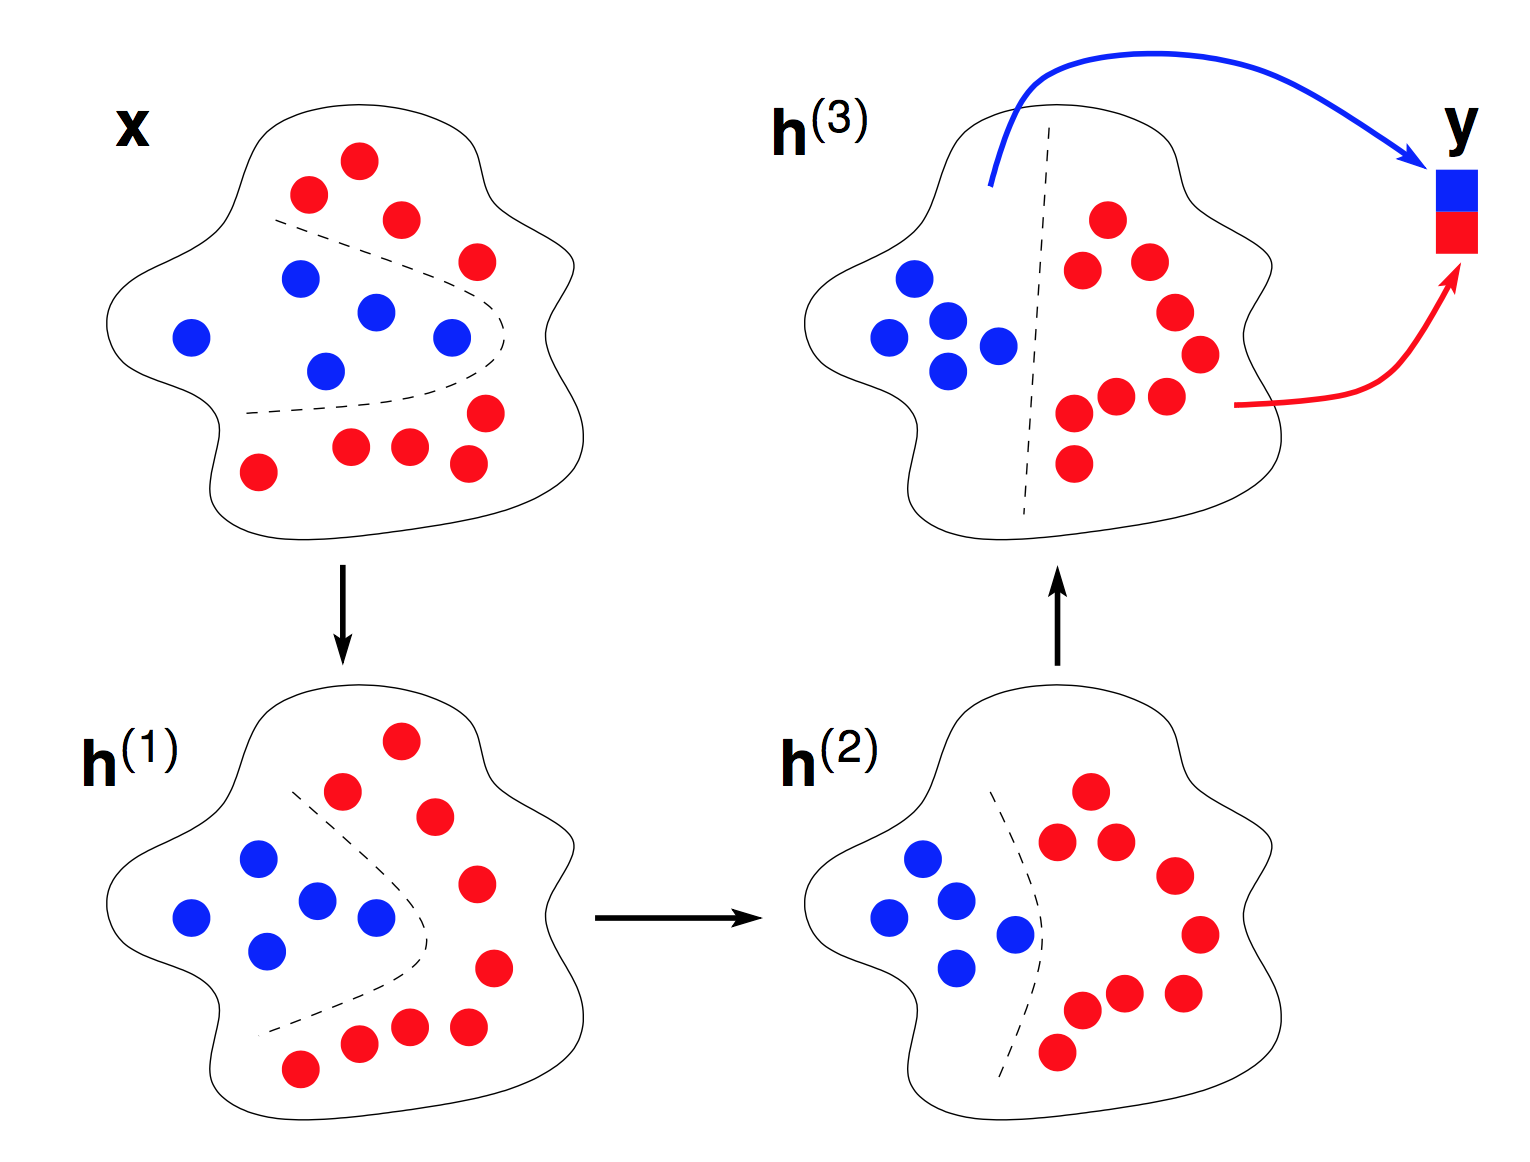
\includegraphics[width=\columnwidth]{figures/adaptive_basis2.png}
    \end{minipage}
    \begin{minipage}{0.39\textwidth}
        \caption{
            \label{fig:feature_extraction_deep}
            The goal of deep learning is to stack many feature extraction
            functions $\phi^l$'s on top of each other to gradually transform the
            problem to become linearly separable. 
        }
    \end{minipage}
\end{figure}

\section{Further Topics$^\star$}

The success of support vector machines does not necessarily come only from the
use of maximum margin principle. Support vector machines are wildly popular when
used together with a kernel technique, which extends a support vector machine to
handle problems that are not linearly separable. Readers are recommended to read
\cite{scholkopf2002learning} by Sch{\"o}lkopf and Smola for more in-depth
discussion of this {\it kernel} support vector machine.

One of the most successful classifiers in practice is a random forest
classifier \cite{breiman2001random}. A random forest classifier consists of many randomly generated
decision trees. Due to the lack of time, we cannot cover decision trees and how
they are used to form a powerful random forest classifier. scikit-learn
implements a random forest classifier, and I highly recommend you to try it out.

Related to the random forest classifier are ensemble methods. 
This family of ensemble methods is focused on how to combine multiple
classifiers in order to achieve better generalization performance. For more
discussion, I suggest you to read Sec.~14.2--3 of \cite{bishop2006pattern}
and/or Sec.~16.2.5 and Sec.~16.4.3 of \cite{murphy2012machine}. 



\chapter{Regression}
\label{sec:regression}

We have so far considered a problem of classification, where the output of a
machine $M$ is constrained to be a finite set of discrete labels/classes. In
this section, we consider a {\it regression} problem in which case the machine
outputs an element from an infinite set.\footnote{
    This definition however is not universal, in that even when the output is
    from a finite set, the problem is sometimes called regression if there
    exists natural ordering of labels.
} A general setup of the problem remains largely identical to that from
Sec.~\ref{sec:supervised_learning}, meaning that it is probably a good idea to
re-read that section at this point.  In the context of regression, we will
particularly focus on framing the whole problem as probabilistic modelling. 

\section{Linear Regression}
\label{sec:linear-regression}

\subsection{Linear Regression}

As we have done with classification, we will start with considering {\it linear
regression}. In linear regression, our machine $M$ is defined as 
\begin{align*}
    M(\vx) = \mW^\top \tilde{\vx},
\end{align*}
where we use $\tilde{\vx}$ to denote the input vector with an extra $1$ attached
at the end.  Similarly to the earlier classification problems, we are given a
set of training examples:
\begin{align*}
    D_{\tra} = \left\{ 
        (\vx_1, \vy_1^*), \ldots, (\vx_N, \vy_N^*)
    \right\}.
\end{align*}
Unlike classification, the output $\vy_n^* \in \RR^q$ is a $q$-dimensional real
vector. 

As should be obvious at this point, the goal of linear regression is to find a
machine, or equivalently its weight matrix, so as to minimize the distance
between the reference machine's output and our machine's output. The reference
machine's outputs are given as a part of the training set.

\paragraph{Distance Function: Log-likelihood Functional}

Given two vectors, one natural way to define the distance between them is a
Euclidean distance which is defined as
\begin{align*}
    \|\vy^* - \vy\|_2^2 = \sum_{k=1}^q (y^*_k - y_k)^2.
\end{align*}
Following our convention, we thus obtain the following distance function for
{\it linear regression}:
\begin{align}
    \label{eq:linreg_dist}
    \Delta(M^*(\vx), M, \vx) = \frac{1}{2} \|M^*(\vx) - M(\vx)\|_2^2 = 
    \frac{1}{2} \sum_{k=1}^q (y^*_k - y_k)^2,
\end{align}
where the multiplicative factor $\frac{1}{2}$ was added to simplify the
gradient.\footnote{
    Why does it simplify anything?
}

At this point of this course, you already know what you need to do. First, you
would define an empirical cost using a training set as
\begin{align*}
    \hat{R}(M, D_{\tra}) = \frac{1}{N} \sum_{n=1}^N
    \|\vy^*_n - M(\vx_n)\|^2_2.
\end{align*}
Then, you would compute the gradient of this empirical cost with respect to the
weight matrix $\mW$ (or more strictly its flattened vector):
\begin{align*}
    \nabla_{\mW} \hat{R}.
\end{align*}
Then, you would use an off-the-shelf optimization algorithm to find a weight
matrix that minimizes the empirical cost function. This would the final step,
right? No! You should use validation to find a correct hypothesis set (or
early-stop learning) to approximately minimize the expected cost function
instead of empirical cost function.

Instead of going this whole pipeline once more in the setting of regression, we
will consider a slightly difference framework in which these machine learning
problems, including both classification and regression, could be embedded. 

\section{Recap: Probability and Distribution}
\label{sec:recap-prob-dist}

Let us briefly go over a few concepts from probability here. They will become
useful in the later discussion where a new framework is introduced. 

\paragraph{Random Variables}

A random variable is not a usual variable in mathematics. A usual variable is
often given a single value. When I say $x=2$, the variable $x$ is equivalent to
the value $2$, and it is equivalent to replacing $x$ with $2$ in any subsequent
equations that include $x$. This is however not true in the case of a random
variable, and sometimes we call a normal variable a {\it deterministic variable}
as opposed to a random variable or a {\it stochastic variable}.

A {\it random variable} is assigned not a single value but a distribution over
all possible values it could take. As an example, consider flipping a coin. We
may declare a random variable $X$ to denote the outcome of flipping a coin. $X$
can then take one of two values $\Omega = \left\{0\text{ (Head)}, 1\text{
(Tail)}\right\}$.  Because we do not know what the outcome would be, we do not
assign $X$ to any one of these values explicitly but assign to it a {\it
distribution} over these two possible choices. 

A distribution is characterized by a function $p$ that maps from one of all
possible values to its corresponding probability, and by a set of constraints on
this function. In this example of coin flipping, $p: \Omega \to \RR$. There are
two constraints on this function $p$. First, the output of this function must be
non-negative:
\begin{align*}
    p(x) \geq 0.
\end{align*}
Second, the probabilities of all possible values must sum to $1$:
\begin{align*}
    \sum_{x \in \Omega} p(x) = 1.
\end{align*}
This function is called a {\it probability mass function}. 

This idea of distribution can be extended to a continuous random variable. A
continuous random variable is assigned correspondingly a {\it continuous
distribution} over a continuous set $\Omega$. Similarly to the definition of a
distribution we defined above for a {\it discrete random variable}, we
characterize a continuous distribution by a function $F$ and a set of
constraints.  Unlike the earlier case, this function $F$ does not return a
probability of a given value, but computes a cumulative probability. That is,
\begin{align}
    \label{eq:cdf}
    F(x) = P(X \leq x),
\end{align}
i.e., what is the probability of a random variable $X$ being less than or equal
to $x$? 

There are two major constraints on this cumulative probability function
$F$.\footnote{
    In addition to two more constraints that are out of scope for this course.
} First, as was the case with the discrete random variable, the value of $F$
must be bounded, and in this case, between $0$ and $1$:
\begin{align*}
    0 \leq F(x) \leq 1, \forall x \in \Omega.
\end{align*}
Second, as the name suggests, this function must be monotonically non-decreasing:
\begin{align*}
    F(x+\epsilon) \geq F(x),
\end{align*}
where $\epsilon > 0$.

Of course, we want something similar to $p$ with a continuous random variable as
well in order to easily mix discrete and continuous random variables. The
definition of the cumulative probability function $F$ in Eq.~\eqref{eq:cdf}
suggests such a function which acts on a single value $x$, rather than a set of
values (i.e. $\left\{ y \in \Omega | y \leq x \right\}$): 
\begin{align*}
    F(x) = \int_{-\infty}^x f(x) \dd{x}.
\end{align*}
This function $f$ is called a {\it probability density function}. 

It is a very bad habit, but a lot of people, including myself, often refer to
both the probability mass function and probability density function simply as a
{\it probability}. This is certainly not correct, but often helps us make our
explanation as well as equations concise, without introducing much, if any,
confusion. Especially, at the level of our discussion in this course, it is
almost always okay to mix them up.\footnote{
    But again, as your instructor, I must insist you know this distinction, and
    will likely ask you to clarify this distinction in the final exam.
}

\begin{figure}[t]
    \begin{minipage}{0.48\textwidth}
        \centering
        \includegraphics[width=\columnwidth]{figures/gauss.pdf}
        (a) Normal Distribution
    \end{minipage}
    \hfill
    \begin{minipage}{0.48\textwidth}
        \centering
        \includegraphics[width=\columnwidth]{figures/gamma.pdf}
        (b) Gamma Distribution
    \end{minipage}
    \caption{
        \label{fig:distributions}
        In these two figures, we plot both a probability density function $f$,
        cumulative density function $F$, the mean and the mode. Additionally, in
        the case of (a) Normal distribution, we coloured the area corresponding
        to the deviation from the mean by one standard deviation.
    }
\end{figure}

\paragraph{Expectation, Variance and Other Statistics}

When a distribution is defined over many possible values, or sometimes
infinitely many values as in the case of continuous random variables, it is
useful to extract a small set of representative values of such a distribution.
This is often what we do in everyday life as well. For instance, when we move to
a new city, we often ask the average monthly rent of an apartment rather than a
full distribution over all possible rent prices. Furthermore, we also want to
know how much a usual monthly rent varies from this average monthly rent so as
not to be surprised. 

First, let us define what we mean by the average X by defining a quantity called
{\it mean}. The mean of a random variable $X$, which has been assigned a
distribution whose probability function is $p$, is defined as
\begin{align*}
    \E\left[ X \right] = \sum_{x \in \Omega} x p(x),
\end{align*}
or in the case of a continuous variable $X$,
\begin{align*}
    \E\left[ X \right] = \int_{x \in \Omega} x p(x) \dd x.
\end{align*}

When we say an ``average'' of a collection of $N$ values, what we often mean is
the following:
\begin{align*}
    \frac{1}{N} \sum_{n=1}^N x_n.
\end{align*}
Can we somehow connect this intuitive definition of average and the new
definition above? 

Indeed we can. This can be done by thinking of $p(x)$ as a frequency of $x$
being selected out of all possible values in $\Omega$. Let's say we have
infinitely many realizations of the random variable $X$. $p(x)$ then corresponds
to how many there are $x$ in this set of infinitely many realizations of $X$,
meaning how frequently $x$ occurred when we observed $X$ infinitely many times.
In this case, multiplying $x$ with the frequency $p(x)$ corresponds to adding
all the occurrences of $x$. By doing this for all possible values of $x$, we end
up with our everyday life definition of ``average''.

Next, let us define {\it variance}. We want to know how far each realization is
from the mean on average. Based on what we have discussed, it should be clear
that
\begin{align*}
    \text{Var}(X) = \sum_{x \in \Omega} (x - \E\left[ X \right])^2 p(x).
\end{align*}
When $X$ is a continuous random variable, we replace the summation $\sum$ with
the integral $\int$. The square-root of the variance is called a {\it standard
deviation}, and is often easier to understand intuitively as it is in the same
scale as the original input $x$. 

Can we generalize this notion of variance further? How about this?
\begin{align}
    \label{eq:central_moment}
    \text{Moment}_p(X) = \sum_{x \in \Omega} (x - \E\left[ X \right])^p p(x).
\end{align}
This is called a {\it $p$-th central moment}, and has turned out to have
interesting properties. For instance, the 3-rd central moment, to which we refer
as {\it skewness}, indicates whether the distribution is symmetric. For
instance, the Normal distribution plotted in Fig.~\ref{fig:distributions}~(a)
has a zero 3-rd central moment, while the Gamma distribution in
Fig.~\ref{fig:distributions}~(b) has a non-zero 3-rd central moment. The 4-th
central moment, called {\it kurtosis}, indicates the flatness of the
distribution with respect to the Normal distribution. Many of these moments have
fascinating use cases in machine learning, but they are out of scope for this
course. 

One interesting observation about the mean is that the mean may not correspond
to an actual value. As a simple example, let us consider a distribution over a
5-star moving rating. Let us assume that {\it a priori} a 5-star moving rating
obeys the following distribution:
\begin{align*}
    p(1) = 0.3, p(2) = 0.2, p(3) = 0.05, p(4) = 0.15, p(5) = 0.3.
\end{align*}
The mean is $2.95$. This number is however not at all informative because of
two reasons.

First, there is no rating of $2.95$. In other words, this is some fantasy number
that summarizes the whole distribution, however, without corresponding to any
real rating. This could be problematic, if our goal is to use this mean to make
a decision or act. For instance, consider placing a bet on predicting the rating
of a newly released movie. I cannot place my bet on $2.95$ but only on one of
those five scores.  Second, even if we decide to round the mean to select the
nearest integer score, we notice that this is far from being representative of
the distribution. The nearest score $3$ has only 5\% chance! 

This latter issue encourages us to define yet another metric called a {\it mode}
of a distribution. A mode of a distribution is a value of which probability is
highest:
\begin{align*}
    \text{Mode}(X) = \argmax_{x \in \Omega} p(x).
\end{align*}
As you can easily guess, a mode is often not unique, and there may be multiple
modes that have the same probability. In fact, a uniform distribution, which
assigns the same probability of each and every possible value, has as many modes
as the size of $\Omega$ (in the case of a continuous random variable, this would
correspond to the infinity.) In practice, we often relax this definition, and
consider all {\it local maxima} as modes of a distribution.

Examples of these statistics with real distributions are presented in
Fig.~\ref{fig:distributions}. 


\paragraph{Distributions}

There are a number of widely used distributions, both discrete and continuous.
As this course is an introduction to machine learning, we will consider only a
small subset of such distributions. 

In the case of discrete variables, we have already learned two popular
distributions. First, we used a {\it Bernoulli distribution} for logistic
regression in Sec.~\ref{sec:logreg}. Bernoulli distribution is defined over a
set of two possible values and fully specified by a single parameter $\mu$:
\begin{align*}
    p(x) = \mu^x (1-\mu)^(1-x),
\end{align*}
where $x \in \left\{ 0, 1\right\}$. The mean of the Bernoulli distribution is
$\mu$, and the variance is $\mu (1-\mu)$. 

Later on in Sec.~\ref{sec:multlogreg}, we extended this Bernoulli distribution
to a {\it categorical distribution} to build a multi-class logistic regression.
Categorical distribution is defined over a set of $C$ possible values, and is
specified by $C$-many probabilities:
\begin{align*}
    p(x) = p_x,
\end{align*}
with a constraint that they are all non-negative and sum to $1$:
\begin{align*}
    &p_x \geq 0, \forall x \in C, \\
    &\sum_{x \in \Omega} p_x = 1.
\end{align*}

In the case of continuous variables, we will solely use a normal distribution,
or often Gaussian distribution, throughout this course. A normal distribution is
defined over an unbounded real vector space $\RR^d$, and is fully specified by
two parameters--mean vector $\mu \in \RR^d$ and covariance matrix $\Sigma \in
\RR^{d\times d}$. Its probability density function is defined as
\begin{align}
    \label{eq:gauss_pdf}
    f(\vx) = \frac{1}{Z} \exp\left( 
        -\frac{1}{2} (\vx - \mu)^\top \Sigma^{-1} (\vx - \mu)
    \right),
\end{align}
where $Z$ is the normalization constant that ensures the integral of the density
function is $1$. That is,
\begin{align*}
    Z &= \int_{\vx \in \RR^d} \exp\left( 
        -\frac{1}{2} (\vx - \mu)^\top \Sigma^{-1} (\vx - \mu)
    \right) \dd \vx \\
    &= (2\pi)^{d/2} |\Sigma|^{1/2},
\end{align*}
where $|\Sigma|$ is the determinant of the covariance matrix.

In practice, and for most of cases throughout this course, we will assume that
the covariance matrix is a diagonal matrix, i.e.,
\begin{align*}
    \Sigma = \left[
        \begin{array}{c c c c}
            \sigma_1^2 & 0 & \cdots & 0 \\
            0 & \sigma_2^2 & \cdots & 0 \\
            \vdots & 0 & \cdots & 0 \\
            \vdots & \vdots & \cdots & \vdots \\
            0 & 0 & \cdots & \sigma_d^2 
        \end{array}
    \right].
\end{align*}
In other words, we assume that each dimension of the input $\vx$ is decorrelated
from each other. In this case, the probability density function simplifies
to\footnote{
    Of course, you may now have noticed that this simplification is left for you
    as a {\bf homework assignment}. 
}
\begin{align}
    \label{eq:gauss_pdf_diag}
    f(\vx) = 
    \prod_{i=1}^d 
    \frac{1}{\sqrt{2\pi} \sigma_i}
    \exp\left(
        -\frac{1}{2} \frac{1}{\sigma_i^2}(x_i - \mu_i)^2
    \right).
\end{align}

\begin{figure}[t]
    \begin{minipage}{0.48\textwidth}
        \centering
        \includegraphics[width=\columnwidth]{figures/joint.pdf}
        (a) Joint Distribution
    \end{minipage}
    \hfill
    \begin{minipage}{0.48\textwidth}
        \centering
        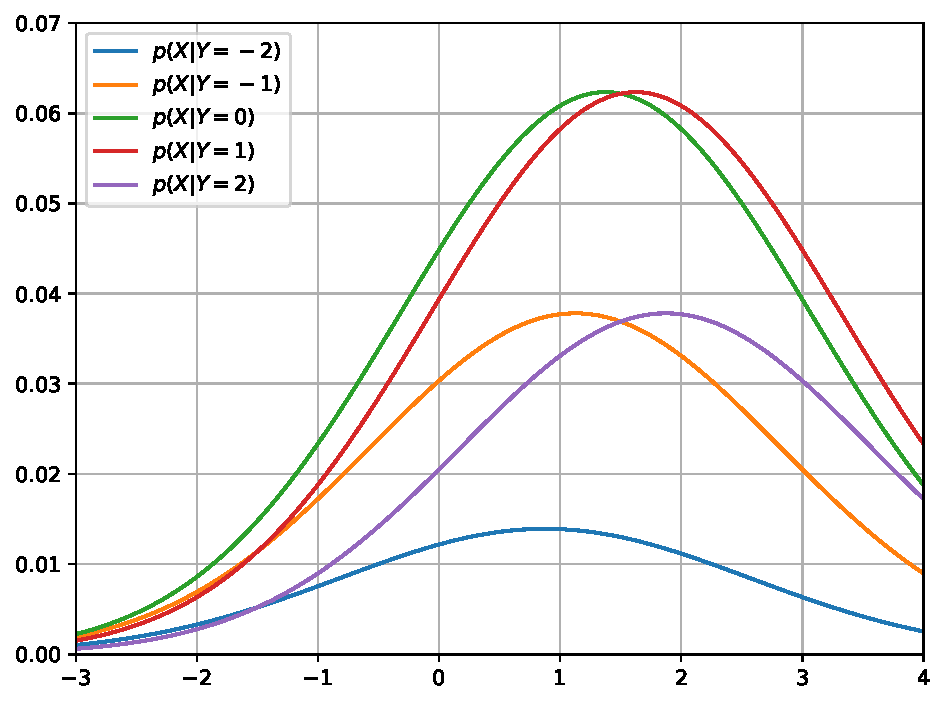
\includegraphics[width=\columnwidth]{figures/conditionals.pdf}
        (b) (Un-normalized) Conditional Distributions
    \end{minipage}
    \caption{
        \label{fig:conditionals}
        In the left figure, we plot the joint distribution over $X$ and $Y$. In
        the right figure, we plot the conditional distributions over $X$ given
        select values of $Y$.
    }
\end{figure}

\paragraph{Bayes' Rule}

Let us consider having two random variables $X$ and $Y$. It is not too difficult
to imagine a joint distribution over them, which could easily be done by
assigning a {\it multivariate} distribution, such as the multivariate normal
distribution from above, to a pair of $X$ and $Y$:\footnote{
    When it is not confusing, we will use $p(x,y)$ as a shorthand notation.
}
\begin{align*}
    p(X=x, Y=y).
\end{align*}
This distribution computes the probability of $X$ and $Y$ having the values $x$
and $y$ respectively. We call this distribution a {\it joint distribution}
between random variables $X$ and $Y$.

Based on this, we can further define a {\it conditional distribution}. A
conditional distribution considers only a subset of all possible joint
probabilities (via the joint distribution) by fixing the value of one random
variable $Y$ to a pre-specified value $y$:
\begin{align*}
    p(X, Y=y).
\end{align*}
In other words, given that the random variable $Y$ is fixed to a value $y$, what
is the distribution over the other {\it free} random variable $X$?

One thing we notice is that the above quantity $p(X, Y=y)$ is not a valid
distribution as it will not sum to $1$ in general. Instead, we need to normalize
it by 
\begin{align*}
    p(X|Y=y) = \frac{p(X, Y=y)}{p(Y=y)}
\end{align*}
to get a proper conditional probability $p(X|Y)$. We often omit $=y$ to denote
that this equation holds regardless of which value $Y$ was assigned to:
\begin{align}
    \label{eq:condprob}
    p(X|Y) = \frac{p(X, Y)}{p(Y)}
\end{align}

From this definition, we can establish one interesting notion of {\it
independence}. If the random variables $X$ and $Y$ are independent from each
other (or mutually independent), then the conditional distribution over $X$
given $Y$ should simply be the distribution over $X$, and vice versa. What does
this notion of independence imply?
If $X$ is independent from $Y$, i.e.,
\begin{align*}
    p(X|Y) = p(X),
\end{align*}
then
\begin{align}
    \label{eq:independence}
    p(X|Y) = p(X) = \frac{p(X, Y)}{p(Y)} 
    \iff p(X, Y) = p(X)p(Y).
\end{align}
In fact, the converse of this statement is also true. That is, if $p(X, Y) =
p(X)p(Y)$, then $X$ and $Y$ are mutually independent.   

These two definitions can easily be mixed in. Consider three random variables
$X$, $Y$ and $Z$. A joint distribution over all of them is $p(X, Y, Z)$. A
conditional distribution over $X$ and $Y$ given $Z$ can be written as $p(X,
Y|Z)$. $X$ and $Y$ are {\it conditionally independent} from each other given
$Z$ {\it iff} 
\begin{align}
    \label{eq:cond_ind}
    p(X,Y|Z) = p(X|Z)p(Y|Z). 
\end{align}

From this definition of conditional distribution, we can compute the conditional
distribution in the opposite direction:
\begin{align}
    \label{eq:bayes-rule}
    p(Y|X) = \frac{p(X|Y)p(Y)}{p(X)}.
\end{align}
This rule is called {\it Bayes' rule}, and it is left for you as a {\bf homework
assignment} to verify that this rule is indeed true. The importance of this rule
will become self-evident in the following sections.

We have so far used $p(X)$ and $p(Y)$ together with a joint distribution
$p(X,Y)$ without establishing their relationship. Of course, the definition of
the conditional probability tells us that 
\begin{align*}
    p(X,Y) = p(X|Y)p(Y),
\end{align*}
but this is simply a circular definition. Instead, can we define $p(X)$ (or
$p(Y)$) on its own based on the joint distribution without resorting to the use
of conditional distribution?  Yes, and we do it by {\it marginalizing out} the
other random variable:
\begin{align}
    \label{eq:marginal}
    p(X) = \sum_{y \in \Omega_Y} p(X, Y=y),
\end{align}
where $\Omega_Y$ is a set of all possible values for $Y$. With this
marginalization, we can rewrite the Bayes' rule in Eq.~\eqref{eq:bayes-rule} as
\begin{align*}
    p(Y|X) = \frac{p(X|Y)p(Y)}{\sum_{Y} p(X, Y)}.
\end{align*}

The usefulness of these probabilistic tools--joint distribution, conditional
distribution, independence, marginalization and Bayes' rule-- will become
self-evident in the following sections, when we start to introduce a so-called
Bayesian approach to machine learning.


\section{Bayesian Linear Regression}
\label{sec:bayesian-linear-regression}

\subsection{Bayesian Linear Regression}

Now that we have refreshed our memory on probability, let us frame what we have
learned so far into this probabilistic terms. For this, we need to define two
distributions; (1) likelihood or a conditional distribution, and (2) a prior
distribution. 

First, let us introduce a new symbol $\theta$ which we will use to denote any
adjustable parameters of a machine. For instance, $\theta$ includes a weight
vector in the case of linear classifiers and linear regression. In the case of
adaptive basis function networks, or deep neural networks, $\theta$ includes a
weight vector, or matrix, as well as all the basis vectors which may be adjusted
to maximize the classification accuracy. All these seemingly diverse set of
adjustable parameters can all be flattened and concatenated to form a single
vector $\theta$. 

Second, let us slightly modify the distance function of linear regression in
Eq.~\eqref{eq:linreg_dist} so as to make it easier to be integrated into a
probability framework. As our motivation speaks for itself, we want to turn the
distance function to be a probability (density) function, similar to what we
have done with logistic regression (see Eq.~\eqref{eq:logreg_dist}.) Unlike
logistic regression, linear regression outputs a continuous value, and therefore
we use a normal distribution in Eq.~\eqref{eq:gauss_pdf} instead of categorical
distribution. For simplicity, we assume that the covariance $\Sigma$ is an
identity matrix:
\begin{align*}
    \Sigma = 
    \left[
        \begin{array}{c c c c}
            1 & 0 & \cdots & 0 \\
            0 & 1 & \cdots & 0 \\
            \vdots & 0 & \cdots & \vdots \\
            \vdots & \vdots & \cdots & \vdots \\
            0 & 0 & \cdots & 1 
        \end{array}
    \right] = \Sigma^{-1}.
\end{align*}
In this case, the probability density function of normal distribution simplifies
to 
\begin{align}
    \label{eq:gauss_pdf_identity}
    f(\vx) = \prod_{i=1}^d 
    \frac{1}{\sqrt{2\pi}}
    \exp\left(
        -\frac{1}{2} (x_i - \mu_i)^2
    \right).
\end{align}

By carefully inspecting this equation and linear regression distance function in
Eq.~\eqref{eq:linreg_dist}, we notice that the latter appears as it is in the
former. Furthermore, by replacing $x_i$ with the $i$-th component of a
ground-truth output $y^*_i$ and $\mu$ with the output of our current machine
$M$, we notice that minimizing the linear regression distance function is
equivalent to maximizing the {\it log}-probability density of this Normal
distribution. That is,
\begin{align}
    \label{eq:linreg_nll}
    \argmin_{M \in H} \Delta(M^*(\vx), M, \vx) =&
    \argmin_{M \in H} -\log f(M^*(\vx); \mu=M(\vx)) \\
    =&\argmin_{M \in H} \sum_{i=1}^q \frac{1}{2} (y^*_i - \mu_i)^2 + C,
\end{align}
where $C$ is a constant that does not depend on $M$, and the constant
multiplicative factor $\frac{1}{2}$ does not change the optimization problem.

In other words, we can rewrite the distance function of linear regression as a
negative log-probability of a ground-truth output vector $y^*$ under a normal
distribution whose mean is the output of the current machine $M$ and covariance
is an identity matrix. So, we have somehow turned linear regression into a
probabilistic model. Let us continue.


\paragraph{Likelihood $p(D|\theta)$}

If we consider this $\theta$ and an entire training set $D=D_{\tra}$\footnote{
    I will use $D$ instead of $D_{\tra}$ throughout the remainder of this
    section for brevity.
} as random variables, a notion of how likely the training set, or the set of
training examples, is given some $\theta$. This is precisely what conditional
probability is (see Eq.~\eqref{eq:condprob},) and we call this specific
conditional probability $p(D|\theta)$ a {\it likelihood}. How does this
likelihood look like?

In this course, we have implicitly assumed that each training input vector $x_n$
(and consequently the corresponding reference output $y_n^*$) was independently
drawn from a single data distribution (see Eq.~\eqref{eq:expected_loss0} from
long time ago.) Then, based on the definition of conditional independence in
Eq.~\eqref{eq:cond_ind}, we can decompose the likelihood into
\begin{align*}
    p(D|\theta) = \prod_{n=1}^N p((x_n, y^*_n)|\theta) 
    = \prod_{n=1}^N p(y^*_n|x_n, \theta) p(x_n | \theta)
    = \prod_{n=1}^N p(y^*_n|x_n, \theta) p(x_n).
\end{align*}
The logarithm of this likelihood, to which we refer as {\it log-likelihood}, is
then 
\begin{align*}
    \log p(D|\theta) = C+ \sum_{n=1}^N \underbrace{\log p(y^*_n | x_n, \theta)}_{(a)},
\end{align*}
where 
\[
    C = \sum_{n=1}^N \log p(x_n)
\]
is a constant with respect to $\theta$.  Where have we seen (a) before? 

Yes, we have seen it twice already this course. We saw one when we defined the
distance functions of logistic regression and multi-class classification, and we
just saw this for linear regression right above in Eq.~\eqref{eq:linreg_nll}.
We have just had a glimpse of an interesting relationship between the likelihood
(or its logarithm version, log-likelihood) and the empirical cost function. That
is, if the distance function of a model could be described in terms of
a probability function, we can define an equivalent log-likelihood
functional.\footnote{
    A {\it functional} is informally-speaking a mapping from a function to a
    scalar. Both the distance function and log-likelihood are functional in that
    the input to them is a function $M$. However, we can equivalently think of
    them as functions by considering the parameters $\theta$ of $M$ as their
    input. This view is enough for the content of this course, but does not hold
    true in general.
} 

\paragraph{Prior $p(\theta)$}

Before we observe a training set $D$, or data, what kind of prior knowledge do
we have about the parameters of a machine? Or, similarly what kind of prior
information do we want to impose on the parameters? The answer to the former
question may be problem-specific, while that to the latter may be
algorithm-specific. A prior distribution is our way to impose or incorporate
such prior knowledge. 

Unlike the likelihood, the prior distribution $p(\theta)$ is defined solely on
the parameters $\theta$ irrespective of actual data $D$. One of the most widely
used prior distributions is again a normal distribution often with an all-zero
mean vector and a diagonal covariance matrix, as in
Eq.~\eqref{eq:gauss_pdf_diag}.\footnote{
    Now you see why I introduced a normal distribution only when we were
    discussing about common distributions.
} Intuitively, this choice of prior distribution states that each parameter is
unlikely to deviate too much from $0$, and how far it may deviate depends on the
variance $\sigma^2$.\footnote{
    Notice the lack of the subscript $i$. We assume that each and every
    parameter $\theta_i$ has the same variance $\sigma$.
}
Mathematically, we express this prior distribution by
\begin{align*}
    p(\theta) = \prod_{i=1}^{|\theta|} \frac{1}{\sqrt{2\pi} \sigma} \exp \left(
    -\frac{\theta_i^2}{2 \sigma^2} \right),
\end{align*}
where $|\theta|$ is the dimensionality of the vector $\theta$. The logarithmic
form is 
\begin{align}
    \label{eq:logprior_gauss}
    \log p(\theta) = 
    \sum_{i=1}^{|\theta|} 
    -\frac{\theta_i^2}{2\sigma^2} - \log \sqrt{2\pi} \sigma.
\end{align}
What does this remind you of?

Of course, this is not the only choice, and we can freely
choose a prior distribution so as to impose certain structures. For instance, if
we believe the first and second parameters are strongly correlated with each
other, we may choose to abandon the diagonal covariance matrix and instead use a
covariance matrix where the cross-correlation term between the first and second
parameters is a large positive value. But, we will get to this later
(hopefully!)

\paragraph{Posterior $p(\theta | D)$}

At the end of the day, we have two goals in machine learning. First, we want to
figure out what the parameters of a model look like once trained. We tackled
this problem earlier by minimizing the empirical cost function (with some
regularization, as in Sec.~\ref{sec:regularization}). In a probabilistic
framework, however, we are rather interested in a {\it posterior} distribution
over the parameters {\it given} a training set: $p(\theta | D)$. 

Unlike the likelihood and prior, we will not designate the form of this
posterior distribution ourselves. Because we already have the likelihood and
prior distribution, we can instead compute the posterior distribution from them
using Bayes' rule in Eq.~\eqref{eq:bayes-rule}:
\begin{align*}
    p(\theta | D) = \underbrace{p(D|\theta)}_{\text{likelihood}}
    \underbrace{p(\theta)}_{\text{prior}}
    \left/
    \underbrace{p(D)}_{\text{evidence}}
    \right..
\end{align*}
Clearly, we need one more distribution $p(D)$, to which we refer as {\it
evidence}. Or, do we?\footnote{
    The following two questions are left for you as {\bf homework assignments}.
    \begin{enumerate}
        \item Why do we call this distribution, or the probability of data $D$,
            evidence? 
        \item Do we need to define this evidence distribution ourselves? If not,
            what can we do about it?
    \end{enumerate}
}

Similarly to the likelihood, it is common to consider the {\it log}-posterior:
\begin{align*}
    \log p(\theta | D) = \log p (D|\theta) + \log p(\theta) - \log p(D).
\end{align*}
Other than the log-evidence $\log p(D)$, let's try to plug in what we know in
the case of linear regression to the right-hand side of this log-posterior:
\begin{align*}
    \log p(\mW | D_{\tra}) = 
    \underbrace{
        \sum_{n=1}^N 
        \log p(\vx_n) + 
        \sum_{i=1}^q 
        -\frac{1}{2} (y^*_{n,i} - [\mW^\top \vx_n]_i )^2 
        - \log \sqrt{2\pi}
    }_{=\log p (D|\theta)}
    +
    \underbrace{
        \sum_{i=1}^{d} 
        \sum_{j=1}^{q}
        -\frac{ w_{ij}^2}{2\sigma^2} - \log \sqrt{2\pi}\sigma
    }_{=\log p(\theta)}
    - 
    \log p(D_{\tra}).
\end{align*}

\paragraph{Maximum-a-Posteriori (MAP) Estimation: Poor Man's Bayes}

Given this form of the log-posterior distribution, what should we do? The first
thing that comes to my mind is to find the parameter vector $\theta$, or
correspondingly the weight matrix $\mW$, that maximizes this posterior
probability. That is, we want to find a {\it mode} of the posterior
distribution:
\begin{align*}
    \hat{\theta} = \argmax_{\theta} \log p(\theta | D) = 
    \argmax_{\theta} \log p(D|\theta) + \log p(\theta) - \log p(D).
\end{align*}
In the case of linear regression, this equation is equivalent to
\begin{align*}
    \argmax_{\theta} \log p(\mW | D_{\tra}) =& 
    \argmax_{\theta} 
        \sum_{n=1}^N 
        \log p(\vx_n)
        +
        \sum_{i=1}^q 
        -\frac{1}{2} (y^*_{n,i} - [\mW^\top \vx_n]_i )^2 
        - \log \sqrt{2\pi}
    +
        \sum_{i=1}^{d} 
        \sum_{j=1}^{q}
        -\frac{w_{ij}^2}{2\sigma^2} - \log \sqrt{2\pi}\sigma
    - 
    \log p(D) \\
    \\
    =&
    \argmax_{\theta} 
        \sum_{n=1}^N \sum_{i=1}^q 
        -\frac{1}{2} (y^*_{n,i} - [\mW^\top \vx_n]_i )^2 
        - \log \sqrt{2\pi}
    +
        \sum_{i=1}^{d} 
        \sum_{j=1}^{q}
        -\frac{w_{ij}^2}{2\sigma^2} - \log \sqrt{2\pi}\sigma
    - 
    \log p(D) \\
    =&
    \argmax_{\theta} 
        \sum_{n=1}^N \sum_{i=1}^q 
        -\frac{1}{2} (y^*_{n,i} - [\mW^\top \vx_n]_i )^2 
        -
        \sum_{i=1}^{d} 
        \sum_{j=1}^{q}
        \frac{1}{2\sigma^2} w_{ij}^2  \\
    =&
    \argmin_{\theta} 
    \underbrace{
        \sum_{n=1}^N \sum_{i=1}^q 
        \frac{1}{2}
        (y^*_{n,i} - [\mW^\top \vx_n]_i )^2 
    }_{\text{Empirical Cost}}
        +
    \underbrace{
        \frac{C}{2} \sum_{i=1}^{d} 
        \sum_{j=1}^{q}
        w_{ij}^2,
    }_{\text{Regularization}}
\end{align*}
where $C=\frac{1}{\sigma^2}$.  Notice that the log-partition functions $\log
\sqrt{2\pi}$'s and the log-evidence $\log p(D)$ have been removed, as they are
not dependent on the parameters $\theta$. 

By carefully inspecting the above equation, especially the final form, we notice
that this is identical to the empirical cost function of linear regression
augmented with a regularization term. More specifically, the regularization term
is the maximum margin regularization term we learned earlier from support vector
machines in Sec.~\ref{sec:svm}. In other words, this probabilistic formulation
of linear regression has resulted in a more traditional formulation of machine
learning we have discussed so far, in the terms of empirical cost function and
regularization. 

Does this mean that all we have done during the past one and a half week has
been to simply find a different way to end up with the exact same solution we
have already learned? That would have been an awful waste of our time, wouldn't
it?


\paragraph{Predictive Distribution $p((x^\star, y^\star)|D)$}

Now we go one step further. In supervised machine learning, what is our ultimate
goal? Was it to find the parameters that minimize the empirical cost function
together with a regularization term? In some cases, yes.  Our goal was however
to build a machine that can predict the outcome of a future, unseen input vector
as well as possible. 

Can we push this even further? Perhaps what we want is only to know the outcome
of a new, unseen input vector. If we can do so, do we really care about
specifically which machine (equivalently, which set of parameters) has been
used? Indeed, we may want to use more than one machines to make their own
predictions and return us their (weighted) consensus. We discussed this
possibility already at the very beginning of this course in
Eq.~\eqref{eq:bayes0}. 

Eventually, what we want to know the conditional distribution over the new
example $(x^\star,y^\star)$ given the training set.\footnote{
    Note that $y^\star$ would not be given together with $x^\star$, but if we
    know their joint distribution $p(x^\star, y^\star|D)$, we can get the
    conditional distribution over $y^\star$ given $x^\star$ according to the
    definition in Eq.~\eqref{eq:condprob}. Of course, in the case of supervised
    learning, we probably want to compute $p(y^\star|x^\star, D)$ directly.
} 
We can do this by {\it marginalizing} out the parameters $\theta$. As we have
seen earlier in Eq.~\eqref{eq:marginal}, we can do so by
\begin{align*}
    \begin{array}{l r}
        p((x^\star, y^\star)|D) & \\
        = \sum_{\theta \in \Theta} p(x^\star, y^\star, \theta|D) &
        \text{marginalization} \\
        = \sum_{\theta \in \Theta} p(x^\star, y^\star|\theta,D)p(\theta|D) &
        \text{conditional probability} \\
        = \sum_{\theta \in \Theta} p(x^\star, y^\star|\theta)p(\theta|D), &
        \text{conditional independence} 
    \end{array}
\end{align*}
where we assumed in the last line that the distribution over an example is
independent from all the other examples {\it given} a set of parameters.
$\Theta$ is a set of all possible sets of parameters.  Examining the final form
further, we notice that it is the expectation of the likelihood under the
posterior distribution over the parameters:
\begin{align*}
    p((x^\star, y^\star)|D) =
        \sum_{\theta \in \Theta} 
        \underbrace{
            p(x^\star, y^\star|\theta)
        }_{\text{Likelihood}}
        \underbrace{
            p(\theta|D)
        }_{\text{Posterior}}
        = \E_{\theta|D} \left[ p(x^\star, y^\star|\theta) \right].
\end{align*}
We call this resulting distribution a {\it predictive distribution}.

What does this equation imply intuitively? The answer is quite straightforward.
We will let each machine, parametrized by $\theta$, cast a vote by scoring each
possible answer $y$ given a new input vector $x^\star$. Their votes are however
not equal, and the votes by those parameters, or equivalently models, which are
more likely given the training data $D$ (i.e., higher posterior $p(\theta | D)$)
would be weighted more. In other words, those machines that do better in terms
of empirical cost function are given higher weights than those that do worse.
The term $\omega(M)$ in Eq.~\eqref{eq:bayes0} thus corresponds to the posterior
probability of $M$ (equiv. to $\theta$). 

As an extra-credit {\bf homework assignment}, you are asked to derive a
closed-form probability density function of the predictive distribution in the
case of linear regression. Linear regression with this derived predictive
distribution is at the heart of {\it Bayesian linear regression}.


\begin{figure}[t]
    \centering
    \begin{minipage}{0.48\textwidth}
        \centering
        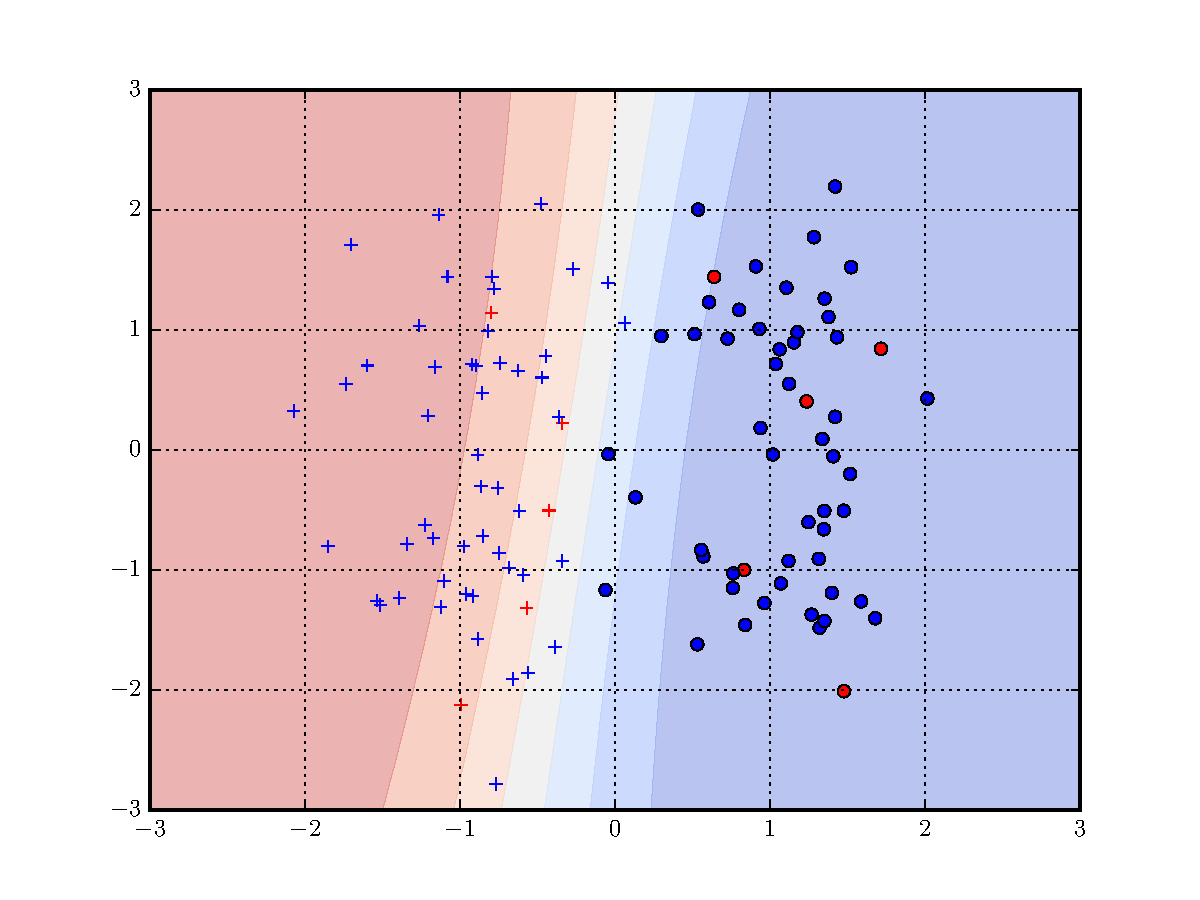
\includegraphics[width=\columnwidth,clip=True,trim=50 0 50
        0]{figures/bayes_logreg.pdf}

        (a)
    \end{minipage}
    \hfill
    \begin{minipage}{0.48\textwidth}
        \centering
        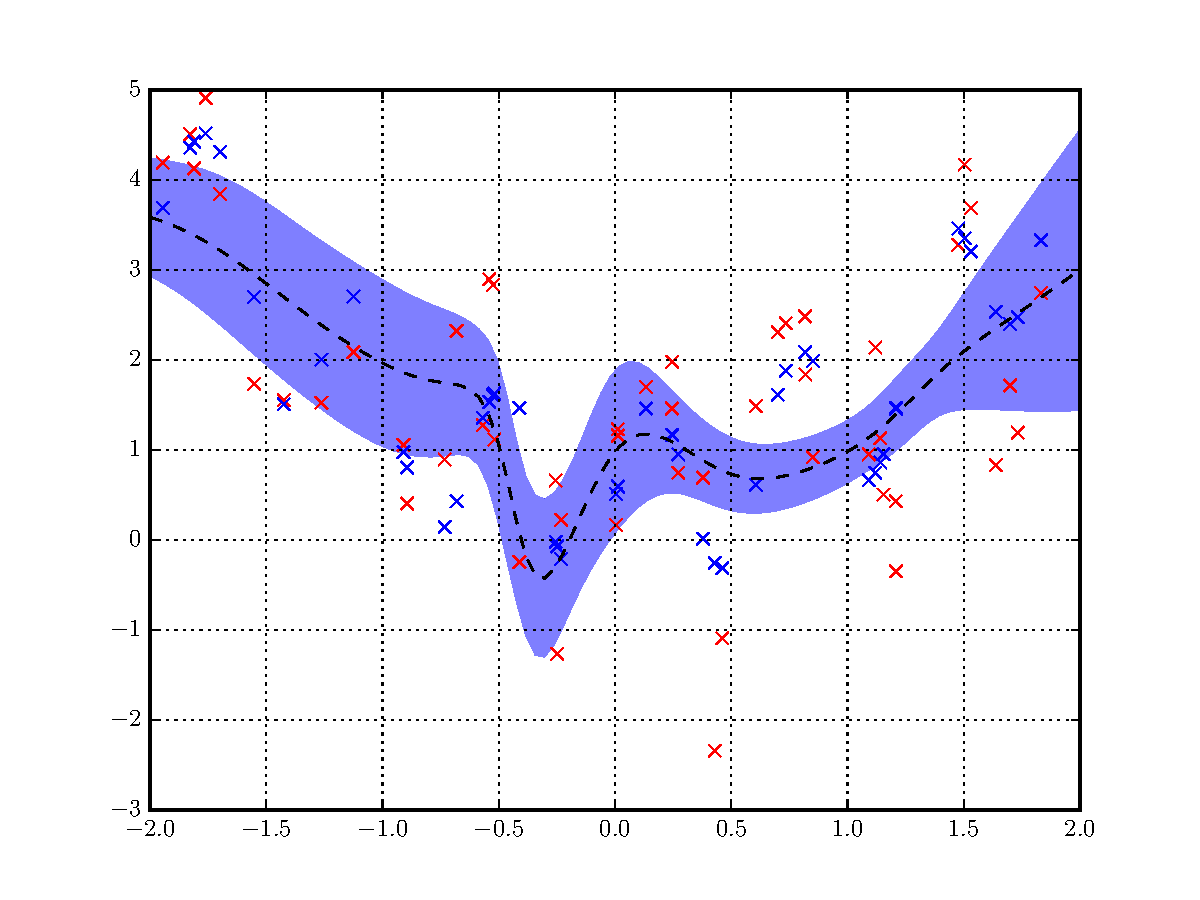
\includegraphics[width=\columnwidth,clip=True,trim=50 0 50
        0]{figures/bayes_linreg_mlp.pdf}

        (b)
    \end{minipage}

    \caption{
        \label{fig:bayes_logreg}
        (a) Bayesian logistic regression, and (b) Bayesian multilayer
        perceptron. Both of them were done with ``ensemble samplers with affine
        invariance'' \cite{goodman2010ensemble} using Python emcee available at
        \url{http://dan.iel.fm/emcee/current/}. 
    }
\end{figure}


\subsection{Bayesian Supervised Learning}

Although we have used linear regression as an example\footnote{
    We call linear regression under this probabilistic approach a {\it Bayesian
    linear regression}.
}
throughout the whole discussion on this probabilistic approach to machine
learning, it should have been clear that this idea is generally applicable as
long as we define the following distributions:
\begin{itemize}
    \item Prior distribution over the parameters: $p(\theta)$
    \item Likelihood distribution: $p(D|\theta)$
\end{itemize}
From these two distributions and a training set $D$, we can derive the posterior
distribution $p(\theta | D)$, and compute the predictive distribution. 

Of course, this is not strictly true in that in almost all cases, we do not know
how to compute the posterior distribution and/or predictive distribution
exactly. Fortunately with linear regression, we were able to do so, but as soon
as we encounter some non-trivial prior and/or likelihood distributions, it is
impossible to derive an analytical form of either posterior or predictive
distribution. 

Thus, to be more precise, in addition to defining those two distributions above,
we need to be able to compute, either exactly or approximately, the posterior
distribution.\footnote{
    When I say {\it compute a distribution}, I mean that being able to (1)
    compute the (unnormalized) probability and (2) compute the expectation and
    the $n$-th central moments in Eq.~\eqref{eq:central_moment}.
} There are two major, general approaches to this problem of computing the
posterior distribution. The first one is a sampling-based approach by which we
can generate samples from a given distribution one at a time with an asymptotic
guarantee that the collected samples are from the given distribution. The most
widely used family of sampling-based algorithms is called Markov-Chain
Monte-Carlo (MCMC). The second approach is variational inference in which a
simpler approximate posterior distribution is fitted to the complex, but true
posterior distribution. Once this simpler approximate distribution is found, we
use it for any subsequent task including the computation of the predictive
distribution. There are a number of other approaches, such as message passing
(or belief propagation) that could be used. Unfortunately any of these
approaches are far out of scope of this course.\footnote{
    I recommend \cite{bishop2006pattern} for further discussion.
}

Instead, let me show you two examples in Fig.~\ref{fig:bayes_logreg}. On the
left panel is the visualization of the predictive distribution of Bayesian
logistic regression. The background gradient indicates the predictive
probability of $y=1$ given a training set (blue markers); red close to $1$, and
blue close to $0$. We notice that the confidence, which can be thought of as how
far away the predictive probability of $y=1$ is from $0.5$, is lower near the
decision boundary. Furthermore, we notice that the low-confidence region grows
as a new input vector is further away from the training examples.

On the right panel is the example of Bayesian multi-layer regression which is
the regression version of the adaptive basis function network from
Sec.~\ref{sec:adfn}. The plot shows both training examples, the mean of the
predictive distributions as well as its standard deviation (shaded region
surrounding the mean curve.) A noticeable feature is that the standard deviation
shrinks when there are many training examples nearby, and grows in the other
case. 

Both examples were done using a specific MCMC algorithm to generate many samples
from the posterior distribution.


\subsection{Further Topic: Gaussian process regression$^\star$}

In linear regression, when the prior distribution over the parameters is
Gaussian and the likelihood is also Gaussian, the posterior distribution over
the parameters as well as the predictive distribution are both Gaussian, due to
the property of multivariate Gaussian distribution. It implies that we can fully
characterize the prediction of a new input example given a training set by
computing the mean and covariance of multivariate Gaussian distribution. The
covariance matrix is often specified by a {\it covariance function}, and a
suitable choice allows us to turn the linear regression into {\it nonlinear}
regression. Unfortunately, Gaussian process regression is out of this course's
scope, and I refer readers to a widely read textbook \cite{williams2006gaussian}
by Williams and Rasmussen, and a great introduction tutorial\footnote{
    \url{http://videolectures.net/gpip06_mackay_gpb/}
}
by David MacKay.





\chapter{Dimensionality Reduction and Matrix Factorization}
\label{chap:dimred}


\section{Dimensionality Reduction: Problem Setup}
\label{sec:dimred}

Let us assume that we are given a set of input vectors without their
corresponding labels. What can we do about these input vectors 
\begin{align*}
    D=\left\{
    \vx_1, \ldots, \vx_N
\right\}?
\end{align*}
Perhaps, the first thing we should try is to look at all of these input vectors
to see if we can find any interesting regularity behind them. If they are
two-dimensional vectors, we can visualize them by plotting a two-dimensional
scatter plot in which each vector is drawn as a single point. If they are
three-dimensional vectors, we can still visualize them by plotting a
three-dimensional scatter plot or by plotting a contour plot. This is however
not as trivial as plotting two-dimensional points. If they are four-dimensional
vectors, already we run out of any ``general'' way to visualize them.

When we are presented with high-dimensional vectors, we try to reduce their
dimensionality in order to (1) visualize them more easily, and (2) more
efficiently process them.\footnote{
    Why is it more efficient to process data points if they are
    lower-dimensional vectors? This question is left to you as a {\bf homework
    assignment}.
} There is a family of machine learning techniques dedicated to this problem of
reducing the dimensionality of input vectors. Applying one of these techniques
is called {\it dimensionality reduction}.

In dimensionality reduction, given a set of input vectors 
\begin{align*}
    D=\left\{
    \vx_1, \vx_2, \ldots, \vx_N
\right\}
\end{align*}
our goal is to find a set of corresponding lower-dimensional vectors
\begin{align*}
    \tilde{D} = \left\{
        \vz_1, \vz_2, \ldots, \vz_N
    \right\},
\end{align*}
where $\vx_i \in \RR^d$, $\vz_j \in \RR^q$, and $d \gg q$. 

There are two major families of techniques in dimensionality reduction. First,
there are parametric dimensionality reduction techniques. Similarly to
supervised learning we have learned earlier, we obtain a machine $M$ that either
maps from an input vector to its corresponding lower-dimensional vector 
\[
    M: \RR^d \to \RR^q,
\]
or maps
from a lower-dimensional vector to its corresponding higher-dimensional
vector\footnote{
    Note that finding either of these two mappings is equivalent when such a
    mapping is invertible. We will discuss this more in detail later when we
    introduce a deep autoencoder. 
}
\[
    M: \RR^q \to \RR^d.
\]
Again, as we learned with supervised learning, this type of machine may be
categorized into either linear or nonlinear. In the case of linear, parametric
dimensionality reduction, the problem can be formulated as {\it matrix
factorization}. On the other hand, nonlinear, parametric dimensionality
reduction is more general, and we will discuss one particular instantiation,
called a {\it deep autoencoder} later in this chapter.

The other family of dimensionality reduction techniques consists of
non-parametric techniques. A non-parametric dimensionality reduction technique
does not provide a separate machine that could be used on a new example, but
only returns a set of lower-dimensional vector $\tilde{D}$. These techniques are
often strictly used for {\it visualization} of high-dimensional data. 

In this course, we will mainly focus on the parametric family of dimensionality
reduction techniques, starting from matrix factorization and ending with deep
autoencoders. If time permits, we will study some non-parametric dimensionality
reduction techniques that are widely used in the scientific community.


\section{Matrix Factorization: Problem Setup}

Let us build a large matrix that contains all the input vectors by lining them
next to each other. That is,
\begin{align*}
    \mX = \left[ \vx_1; \vx_2; \cdots \vx_N \right] \in \RR^{d \times N}.
\end{align*}
{\it Matrix factorization} is then a problem of (approximately) representing
this data matrix $\mX$ as a product of two matrices:
\begin{align}
    \label{eq:matfac}
    \mX \approx \mW \mZ,
\end{align}
where $\mZ$ is a matrix that contains all the lower-dimensional vectors
\begin{align*}
    \mZ =\left[ \vz_1; \vz_2; \cdots; \vz_N \right],
\end{align*}
and $\mW \in \RR^{d \times q}$ is a weight matrix. $\mZ$ is often called a code
matrix, and $\mW$ a dictionary matrix.  By setting $q$ to be smaller than $d$,
i.e., $q \ll d$, this matrix factorization allows us to find a set of
lower-dimensional vectors. In other words, matrix factorization allows us to
reduce the dimensionality of input vectors.

Matrix factorization is a widely-used, and perhaps oldest, dimensionality
reduction technique. It is a {\it linear} dimensionality reduction technique, as
evident from Eq.~\eqref{eq:matfac}. Why is this so? Because, the equation in
Eq.~\eqref{eq:matfac} could be understood as a set of $N$ equations of which
one is
\begin{align}
    \label{eq:matfac1}
    \vx_i = \mW \vz_i.
\end{align}
Matrix factorization is precisely a way to build a {\it linear} machine that
maps from a lower-dimensional vector to its original space $\RR^d$. 

Eq.~\eqref{eq:matfac1} reminds us of linear regression in
Sec.~\ref{sec:linear-regression}. The only difference is that both $\vz$ and
$\vx$ were known in linear regression, while only one of them, $\vx$, is known
in matrix factorization. This lack of input vectors, following the terminology
from linear regression, implies that this problem is under-specified, meaning
that there may be many solutions of $\mW$ and $\mZ$ that satisfy
Eq.~\eqref{eq:matfac}. This is quite obvious, if we consider the simplest case
of $d=q=1$, in which case the whole problem reduces to finding $w$ and $z$ that
satisfies
\begin{align*}
    x = w z,
\end{align*}
where $x$ is known. For any solution $(w, z)$ that satisfies this equality,
there are infinitely many other solutions $(w', z')$ such that
\begin{align*}
    w' = cw\text{ and }
    z' = \frac{z}{c},
\end{align*}
where $c$ is an arbitrary real number. A similar thing happens with $d, q > 1$
with any invertible matrix $\mC \in \RR^{q \times q}$, because
\begin{align*}
    \mX = (\mW \mC)(\mC^{-1} \mZ) = \mW (\underbrace{\mC \mC^{-1}}_{=\mI}) \mZ = \mW \mZ.
\end{align*}

What this implies is that there are many different ways to solve this matrix
factorization. By imposing a set of clever constraints on the weight matrix
$\mW$ and/or $\mZ$, we get a diverse set of linear dimensionality reduction
algorithms. In the rest of this section, we investigate three such algorithms. 


\subsection{Principal Component Anslysis: Traditional Derivation}
\label{sec:pca}

The first such algorithm is called principal component analysis (PCA). In PCA,
there are two constraints. The first constraint is on $\mZ$, or a set of code
vectors $\vz_1, \ldots, \vz_N$. It states that each component of these code
vectors must be {\it decorrelated} from all the other components. This is
equivalent to 
\begin{align*}
    \sum_{n=1}^N z_{j,n} z_{i,n} = 0,\text{ for all }i \neq j,
\end{align*}
assuming that $\vz_n$'s are centered. We can write it more compactly by
\begin{align*}
    \mZ \mZ^\top = \sum_{n=1}^N \vz_{n} \vz_n^\top = \diag(\sigma_1^2, \ldots, \sigma_q^2),
\end{align*}
where 
\begin{align*}
    \Sigma = \diag(\sigma_1^2, \ldots, \sigma_q^2) = 
    \left[
        \begin{array}{c c c c}
            \sigma_1^2 & 0 & \cdots & 0 \\
            0 & \sigma2^2 & \cdots & 0 \\
            \vdots & 0 & \cdots & \vdots \\
            \vdots & \vdots & \cdots & \vdots \\
            0 & 0 & \cdots & \sigma_q^2 
        \end{array}
    \right].
\end{align*}
The second constraint is that these variances $\sigma_j^2$'s are non-increasing.
In other words, 
\begin{align*}
    \sigma_i^2 \geq \sigma_j^2,\text{ for all }i < j.
\end{align*}

With these constraints in our mind, let us consider the (scaled) covariance of
the input vector matrix $\mX$ which is defined as
\begin{align*}
    \underbrace{\mX \mX^\top}_{\mathclap{\mC=\text{Covariance of }\mX}} =& 
    (\mW \mZ) (\mW \mZ)^\top \\
    =& \mW \underbrace{\mZ \mZ^\top}_{
\mathclap{\Sigma=\text{Covariance of }\mZ}} \mW^\top \\
=& \mW \Sigma \mW^\top
\end{align*}
Since any covariance matrix is by definition symmetric,\footnote{
    A matrix $\mC$ is symmetric if and only if
    \begin{align*}
        \mC = \mC^\top.
    \end{align*}
}
we immediately notice that this equation precisely describes a procedure called
{\it eigendecomposition}:
\begin{align}
    \label{eq:eigendecomp}
    \mC = \mW \Sigma \mW^\top,
\end{align}
assuming $q=d$. $\mW$ is then a matrix consisting of $d$ eigenvectors of
$\mC$ on each column:\footnote{
    We assume that $N \gg d$, and that the subspace in which all the input
    vectors lie is at least $q$-dimensional.
}
\begin{align*}
    \mW = \left[ \vv_1; \vv_2; \cdots; \vv_d \right],
\end{align*}
where
\begin{align}
    \label{eq:eigenvector}
    \mC \vv_j = \sigma_j^2 \vv_j
\end{align}
which is the definition of the $j$-th eigenvector, and $\sigma_j^2$ is the
corresponding $j$-th eigenvalue. These eigenvalues and the corresponding
eigenvectors can be computed by first solving the characteristic polynomial of
$\mC$ to find all eigenvalues and solving Eq.~\eqref{eq:eigenvector} for each of
the eigenvalues.\footnote{
    It is out of the scope of this course to teach how to find eigenvalues and
    eigenvectors. I refer students to take, for instance, MATH-UA 140 LINEAR
    ALGEBRA listed at the Department of Mathematics. 
}
We see that Eq.~\eqref{eq:eigendecomp} is nothing but a stack of
Eq.~\eqref{eq:eigenvector} in the decreasing order of $\sigma_j^2$'s.  In other
words, we can compute the weight matrix $\mW$ by eigendecomposition of the
(scaled) covariance matrix $\mC$ of the input matrix $\mX$.

This is a good start as this selection of the weight matrix $\mW$ ensures that
the code vectors are decorrelated, satisfying the first constraint. But, how do
we compute the code matrix $\mZ$? One important property of the eigenvectors is
that they are orthogonal to each other.\footnote{
    This is true only when the associated eigenvalues are positive. 
} Since the inverse of any orthogonal matrix is its transpose, we can compute
the code matrix by
\begin{align}
    \label{eq:pca_infer}
    \mZ = \mW^\top \mX.
\end{align}

Along the derivation, we have made one assumption that $q=d$. This effectively
means that we have not done any dimensionality {\it reduction}. How do we then
use this whole procedure to reduce the dimensionality, that is $q \ll d$? We can
do it easily by simply taking only the first $q$ columns of the weight matrix, or
taking only the first $q$ eigenvectors. That is,
\begin{align*}
    \mW = \left[
        \vv_1; \vv_2; \cdots; \vv_q
    \right].
\end{align*}
Because the eigenvectors were sorted in the decreasing order of the
eigenvalues which correspond to the variance of each component of the code
vectors, this satisfies the second constraint. Of course, this breaks the
equality in Eq.~\eqref{eq:eigendecomp}, but is still a good approximation, as we
will see shortly.

In summary, PCA is done in the following steps:
\begin{enumerate}
    \item Centering: $\vx_n \leftarrow \vx_n - \frac{1}{N}\sum_{n=1}^N \vx_n$
    \item Covariance: $\mC = \mX \mX^\top$
    \item Eigendecomposition: $\mC = \mW \Sigma \mW^\top$
    \item Top-$q$-column extraction: $\mW \leftarrow \mW_{:,1:q}$
    \item Code vectors: $\mZ = \mW^\top \mX$
\end{enumerate}
Despite the simplicity in description, this whole process is computational
expensive, especially due to the computation of the covariance matrix $\mC$.  It
is therefore desirable to skip computing the covariance matrix, and fortunately
there is a way to do so by resorting to singular value decomposition.

Singular value decomposition (SVD) decomposes a given matrix $\mX$ into a
product of three matrices:
\begin{align}
    \label{eq:svd}
    \mX = \mW \mS \mV,
\end{align}
where $\mW \in \RR^{d \times d}$ and $\mV \in \RR^{d \times N}$ are orthogonal
matrices, and $\mS \in \RR^{d \times d}$ is a diagonal matrix with
decreasing diagonal entries. Let us use this decomposition to compute the
covariance matrix $\mC$:
\begin{align*}
    \mC =& \mX \mX^\top \\
    =& \mW \mS \mV (\mW \mS \mV)^\top \\
    =& \mW \mS \underbrace{\mV \mV^\top}_{=\mI} \underbrace{\mS^\top}_{=\mS} \mW^\top \\
    =& \mW \mS \mS \mW^\top \\
    =& \mW \Sigma \mW^\top.
\end{align*}
Surprised? Yes, the matrix $\mW$ could be precisely recovered by SVD on the
input matrix $\mX$ without computing the covariance matrix. Because of this, it
is common to directly use SVD on the input matrix in practice.

\paragraph{Proportion of Variance Explained: PV}

The variance of the sum of decorrelated random variables is simply the sum of
the variances of all those random variables, i.e.,
\begin{align*}
    \var(\sum_{i=1}^q Z_i) = \sum_{i=1}^q \var(Z_i).
\end{align*}
By considering each component of the code vectors as a random variable, this
implies that the (empirical) variance of the sum of these code components is
simply the sum of the first $q$ eigenvalues: $\sum_{i=1}^q \sigma_i^2$. We can
then compute how much variance has been {\it explained} by the code vectors by
inspecting the ratio between the variance of the code components and the
variance of the whole input:
\begin{align*}
    \text{PV}(q) = \frac{
        \sum_{i=1}^q \sigma_i^2
    }{
        \sum_{j=1}^d \sigma_j^2
    }.
\end{align*}

What does this proportion of variance explained (PV) correspond to? We will see
it in the upcoming demonstration session.

\paragraph{What are principal components?}

The principal components are the column vectors of the weight matrix $\mW$.
They are orthogonal to each other, and form a $q$-dimensional subspace in the
original $d$-dimensional real space $\RR^d$. The code vector $\vz$ of an input
vector $\vx$ is then an orthogonal projection of $\vx$ onto this subspace. This
projection $\vz$ obtained by Eq.~\eqref{eq:pca_infer} then corresponds to the
{\it reconstruction} in the original space by
\begin{align}
    \label{eq:pca_recon}
    \hat{\vx} = z_1 \vw_1 + z_2 \vw_2 + \cdots + z_q \vw_q = \mW \vz.
\end{align}
Note that
\begin{align*}
    z_i = \vw_i^\top \vx.
\end{align*}

With this reconstruction, we can define a {\it reconstruction error} by
\begin{align*}
    \| \vx - \hat{\vx} \|^2_2.
\end{align*}

Now the question is what kind of subspace the procedure above finds. From the
first constraint, that the code vectors are decorrelated with each other, we
know that the principal components are eigenvectors of the input covariance
matrix $\mC$.\footnote{
    Orthonormal vectors are orthogonal to each other and have a unit norm.
} What does the second constraint tell us about our selection of the first $q$
eigenvectors?

First, we notice that we can represent any input vector as a weighted sum of the
eigenvectors, similarly to Eq.~\eqref{eq:pca_recon}:
\begin{align*}
    \vx = z'_1 \vw_1 + z'_2 \vw_2 + \cdots + z'_d \vw_d,
\end{align*}
where 
\begin{align*}
    z'_i = \vw_i^\top \vx.
\end{align*}
The reconstruction error can then be written as\footnote{
    Note that I am looking at a single input vector $\vx$, but this equation
    trivially extends to, and is in fact necessary to have, multiple input
    vectors $\vx_1, \ldots, \vx_N$. For brevity and simplicity, my derivation
    here considers a single input vector, but it is left for you as a {\bf
    homework assignment} to extend this derivation to use multiple input
    vectors.
}
\begin{align*}
    \| \vx - \hat{\vx} \|^2_2 =&
    \left\| \sum_{i=1}^q (z'_i - z_i) \vw_i + \sum_{j=q+1}^d z'_j \vw_j \right\|^2_2 \\
    =& 
    \left\| \sum_{j=q+1}^d z'_j \vw_j \right\|^2_2 \\
    =& 
    \sum_{j=q+1}^d {z'}_j^2 \underbrace{\| \vw_j \|^2}_{=1} \\
    =& 
    \sum_{j=q+1}^d {z'}_j^2 \\
    =&
    \sum_{j=q+1}^d \vw_i^\top \underbrace{\vx \vx^\top}_{
    \mathclap{\mC=\text{covariance}}} \vw_i \\
    =&
    \sum_{j=q+1}^d \vw_i^\top \mC \vw_i.
\end{align*}
Now this looks awfully similar to the eigendecomposition from
Eq.~\eqref{eq:eigendecomp}, where we learned that\footnote{
    It is your {\bf homework assignment} to show that the equations below are
    true.
}
\begin{align*}
    &\Sigma = \mW^\top \mC \mW \\
    \iff&
    \sigma_j^2 = \vw_j^\top \mC \vw_j,\text{ for all }j=1,\ldots,d.
\end{align*}
In other words, the reconstruction error equals to the sum of the eigenvalues of
the discarded eigenvectors:
\begin{align*}
    \| \vx - \hat{\vx} \|^2_2 =
    \sum_{j=q+1}^d \sigma_j^2.
\end{align*}
Thus, we minimize the reconstruction error by selecting the top-$q$ eigenvectors
according to their corresponding eigenvalues as the principal components. If we
want to add one more, we add another eigenvector whose eigenvalue is greater
than equal to that of any other remaining eigenvector.

This view of PCA as finding a subspace that minimizes the reconstruction error
becomes handy when we extend it to nonlinear PCA later. A deep autoencoder,
which is one realization of nonlinear PCA, directly and explicitly minimizes the
reconstruction error.


\subsection{PCA: Minimum Reconstruction Error with Orthogonality Constraint}

We have derived PCA from the two constraints; (1) the elements of a code vector
$\vz$ are decorrelated, and (2) the variances of the elements of a code vector
are sorted in a decreasing order. We have seen that the first constraint led to
the orthogonality of the weight matrix, or the dictionary matrix, $\mW$. The
second constraint, on the other hand, led to the minimum reconstruction error
criterion. This latter revelation tells us that the second constraint of PCA is
perhaps not a criterion on its own, but rather a consequence of optimization
which has been at the core of machine learning so far in this course (except for
the Bayesian linear regression.) 

Here, we will re-formulate PCA by starting with an optimization cost, which
is similar to the empirical cost function we have used throughout our
discussions on supervised learning. The optimization cost function is
defined as the reconstruction error over a given training set $D_{\tra}$:
\begin{align*}
    \hat{R}(\mW, \mZ; D_{\tra}) =& \sum_{n=1}^N \| \vx_n - \hat{\vx}_n
    \|^2_2 \\
    =& \| \mX - \mW \mZ \|_F^2.
\end{align*}
Looking closely at the equation at the bottom, we in fact see that this
corresponds to finding the weight matrix $\mW$ and the code matrix $\mZ$ such
that their product $\mW \mZ$ is close to the input matrix $\mX$, which was the
main goal of matrix factorization from the very beginning as in
Eq.~\eqref{eq:matfac}. 

This minimization alone does not however result in PCA, as naive minimization
would not find a solution that satisfies the first constraint. We therefore
impose that the first constraint be satisfies during optimization. That is, 
\begin{align*}
    \min_{\mW, \mZ} \hat{R}(\mW, \mZ)
\end{align*}
subject to the constraint that
\begin{align*}
    \text{The column vectors of }\mW \text{ are orthonormal vectors}.
\end{align*}
Assuming that this constraint is always satisfied during optimization, we can
now safely replace $\mZ$ with $\mW^\top \mX$, because $\mW^\top \mW = \mI$. This
results in 
\begin{align*}
    \hat{R}(\mW, \mX; D_{\tra}) 
    = \| \mX - \mW \mW^\top \mX \|_F^2
\end{align*}
subject to 
subject to the constraint that
\begin{align*}
    \text{The column vectors of }\mW \text{ are orthonormal vectors}.
\end{align*}

This alternative derivation of PCA gives us a more general framework on top of
which various matrix factorization algorithms could be implemented. In this
general framework, the goal is to minimize the reconstruction error $\| \mX -
\mW \mZ\|_F^p$. This is natural, as our goal is to find the weight and code
matrices whose product is approximately the input matrix. We then need another
mechanism $g$ , or a function, that allows us to map from a given input vector
$\vx$ to its corresponding code vector $\vz$, i.e. $\vz =g(\vx, \mW)$. That is,
we should be able to infer what the code matrix $\mZ$ is given the input matrix
$\mX$ and the weight matrix $\mW$.\footnote{
    Note that $g$ may not be a function, but a process in which the
    reconstruction cost function is minimized with respect to the code matrix
    $\mZ$ (instead of $\mW$). This is a usual practice in sparse coding.  
} 
Then, we need a certain constraint on either the weight matrix $\mW$ and/or the
code matrix $\mZ$. In summary, a matrix factorization algorithm, or framework,
is defined based on the following items:
\begin{enumerate}
    \item Cost function (almost always reconstruction error)
    \item Constraints on $\mW$ and/or $\mZ$
    \item Inference mechanism $g$: infer $\vz$ from $\vx$ given $\mW$
\end{enumerate}
Furthermore, the appropriate choice of constraints relaxes the basic assumption
we had earlier about the dimensionality of the code vector $q$ that it is often
much smaller than $d$. 

To reiterate, in the case of PCA, the cost function is a reconstruction error
defined in terms of Euclidean distance (or Frobenius norm). The inference
mechanism is simply $\vz = g(\vx) = \mW^\top \vx$, and there is a single
constraint that $\mW$ is orthogonal.

Many different matrix factorization algorithms could be formulated under this
framework. For instance, sparse coding \cite{olshausen1997sparse} is defined by
\begin{enumerate}
    \item Cost function: L2 reconstruction error
    \item Constraint: $\| \vz \|_0=k$, for some $k>0$
    \item Inference mechanism: minimization with respect to $\mZ$
\end{enumerate}
It is often the case with sparse coding that $q\gg d$. Independent component
analysis (see, e.g., \cite{hyvarinen2004independent})is on the other hand
defined by
\begin{enumerate}
    \item Cost function: L2 reconstruction error
    \item Constraint: $z_i \bot z_j$, for all $i \neq j$
    \item Inference mechanism: minimization with respect to $\mZ$ or $g(\vx)=\mU
        \vz$
\end{enumerate}
$\mU$ is a matrix separate from $mW$ that recovers the code vector from an input
vector. $\bot$ is used to denote the independence between two random variables
(see Eq.~\eqref{eq:independence}.) Because of different choices of inference
mechanism and constraints, these algorithms often learn different weight
matrices and code matrices even when provided with the same input matrix $\mX$. 

In the next subsection, we will consider another matrix factorization algorithm,
called non-negative matrix factorization, that is capable of learning a
so-called {\it part-based representation}. 


\subsection{Non-negative Matrix Factorization: NMF}
\label{sec:nmf}

Let us consider another matrix factorization scheme called non-negative matrix
factorization~(NMF,~\cite{lee2001algorithms}). Let us go step-by-step here. What
is our main objective? Exactly the objective function we have used for principal
component analysis (PCA):
\begin{align*}
    \hat{R}(\mW, \mZ) = \| \mX - \mW \mZ \|_F^2.
\end{align*}
What kind of constraints do we want? The name itself suggests them. That is,
both the weight matrix $\mW$ and the code matrix $\mZ$ are {\it non-negative}.
Of course, this naturally assumes that the input matrix $\mX$ is also
non-negative, because the sum, product or their combination, of non-negative
numbers would never result in negative. What this implies is that we must ensure
that the input matrix is non-negative by, for instance, subtracting the minimum
value of $\mX$ from $\mX$. This is a preprocessing step that is similar to the
centering step of PCA.

In summary, the optimization problem of NMT is defined as
\begin{align}
    \label{eq:nmf}
    \argmin_{\mW, \mZ} \| \mX - \mW \mZ \|_F^2
\end{align}
subject to
\begin{align*}
    &w_{ij} \geq 0,\text{ for all }i=1,\ldots,d\text{ and }j=1,\ldots,q \\
    &z_{ij} \geq 0,\text{ for all }i=1,\ldots,q\text{ and }j=1,\ldots,N.
\end{align*}
Before learning how to solve this constrained optimization problem, let us
discuss why NMF is an interesting case of matrix factorization. 

As we discussed earlier, the weight matrix $\mW$ is often called a dictionary
matrix. This dictionary matrix contains a set of $q$ atoms:
\begin{align*}
    \mW = \left[ \vw_1; \vw_2; \cdots; \vw_q \right].
\end{align*}
These atoms are then combined according to their coefficients, given by a code
vector, to form one of the input vectors. That is,
\begin{align*}
    \hat{\vx} = z_1 \vw_1 + z_2 \vw_2 + \cdots + z_q \vw_q = \mW \vz.
\end{align*}

Now let's do some quick thought experiment. Input vectors are human faces. What
would be those atoms, when we are constrained to only {\it add} them? In other
words, those positive-valued atoms and their positive-valued coefficients
prevent us from cancelling out the contributions of the atoms. For instance, we
cannot have an atom that has three positive noses and another atom that has two
negative noses so that summing them would leave us only one nose. In order to
build a full face with NMF, we would need to have an atom for a nose, an atom
for a pair of eyes, an atom for a mouth, an atom for a pair of ears and so on.
In other words, each positive-valued atom needs to contain a set of parts of a
face that do not overlap with each other, and each positive-valued coefficient
indicates how much contribution the corresponding atom makes to the full face.

\begin{figure}[t]
    \centering
    \begin{minipage}{0.59\columnwidth}
        \centering
        \includegraphics[width=\columnwidth]{figures/nmf.png}
    \end{minipage}
    \begin{minipage}{0.4\columnwidth}
        \caption{
            \label{fig:nmf}
            A graphical illustration of how non-negative matrix factorization
            models a face as a weighted sum of parts in a dictionary matrix
            $\mW$. The figure was taken from \cite{lee2001algorithms}.
        }
    \end{minipage}
\end{figure}

This is precisely the motivation behind the NMT.
Lee~and~Seung~\cite{lee2001algorithms} showed that if you solve NMF on a set
$\mX$ of (normalized) faces, the dictionary matrix $\mW$ contains face parts
(such as mouth, eyes, nose, and so on), and the code matrix $\mZ$ captures how
some of those parts are selected and combined to form full faces. This process
for one face is shown in Fig.~\ref{fig:nmf}.

Let us do another thought experiment. How about modelling a document? As we did
earlier in Sec.~\ref{sec:feat}, we assume each document is represented as a bag
of words. What would be a good dictionary of atoms in this case? Perhaps each
atom should represent a topic. If a document is about ice hockey, this document
would be a result of adding multiple topics such as sports, hockey and ice.
Again, each of these topics would have to be exclusive, since the non-negativity
constraint prevents us from two atoms to {\it cancel out} each other. Again,
this was one of the examples given in \cite{lee2001algorithms}, as shown in
Fig.~\ref{fig:nmf_doc}.

\begin{figure}[t]
    \centering
    \begin{minipage}{0.59\columnwidth}
        \centering
        \includegraphics[width=\columnwidth]{figures/nmf_doc.png}
    \end{minipage}
    \begin{minipage}{0.4\columnwidth}
        \caption{
            \label{fig:nmf_doc}
            A graphical illustration of how non-negative matrix factorization
            models a document as a weighted sum of topics from a dictionary
            matrix $\mW$. The figure was taken from \cite{lee2001algorithms}.
        }
    \end{minipage}
\end{figure}

The constrained optimization problem for NMF in Eq.~\eqref{eq:nmf} is not a
trivial problem, and many optimization algorithms have been proposed to solve
NMF. Since most of them are way out of the scope of this course, I will briefly
describe a straightforward extension of gradient-descent algorithm, called
projected gradient-descent algorithm. Unlike the usual gradient descent
algorithm, the projected gradient-descent algorithm consists of two steps. The
first step is to update the parameters (in our case, $\mW$ and $\mZ$) following
the negative gradient direction:
\begin{align}
    \label{eq:nmf_dw}
    \tilde{\mW} =& \mW - \eta \nabla_{\mW} \hat{R} = \mW - \eta (\mX - \mW \mZ)
    \mZ^\top, \\
    \label{eq:nmf_dz}
    \tilde{\mZ} =& \mZ - \eta \nabla_{\mZ} \hat{R} = \mZ - \eta \mW^\top (\mX -
    \mW \mZ), 
\end{align}
which is precisely the gradient-descent algorithm. 

The second step (note that we have not updated the actual matrices yet) involves
{\it projecting} these candidate matrices back to a feasible region which
consists of all points that satisfy the constraints. That is, 
\begin{align*}
    \mW = \argmin_{\mW \geq 0} \|\mW - \tilde{\mW}\|^2_F, \\
    \mZ = \argmin_{\mZ \geq 0} \|\mZ - \tilde{\mZ}\|^2_F. \\
\end{align*}
In other words, we want to find, for instance, a weight matrix $\mW$ with all
non-negative values that is close to the updated matrix $\tilde{\mW}$, and the
same for the code matrix $\mZ$. Finding such a projection is generally
difficult, but in the case of NMF, the projection is simply
\begin{align*}
    w_{ij} =& \max(0, \tilde{w}_{ij}), \\
    z_{ij} =& \max(0, \tilde{z}_{ij}). \\
\end{align*}
That is, we simply cut off any negative values from both the weight matrix and
code matrix.  This projected gradient algorithm is widely used for non-negative
matrix factorization in addition to the original multiplicative update rules
from \cite{lee2001algorithms}.

We will see NMF in action during the next demonstration session.




\section{Deep Autoencoders: Nonlinear Matrix Factorization}

A major limitation of matrix factorization $\mX \approx \mW\mZ$ is that the
relationship between a code vector $\vz$ and its corresponding input vector
$\vx$ is {\it linear}. Given a fixed dimensionality $q$ of a code vector, what
happens if there is no good linear map from it to the corresponding input
vector? Perhaps what we need is to relax this linearity assumption. That is,
\begin{align*}
    \vx = f_{\theta}(\vz),
\end{align*}
where $f_{\theta}$ is a nonlinear function parametrized by a set $\theta$ of
parameters. We can use, for instance, a {\it deep} feature extraction function
(or deep neural network) from Sec.~\ref{sec:adfn}.

As usual with the other matrix factorization methods above, we first define a
cost function as a reconstruction error. A usual one is Euclidean distance as
below:
\begin{align*}
    \hat{R}(\theta, \mZ) = \frac{1}{N} \sum_{n=1}^N \| \vx - f_{\theta}(\vz) \|^2_2.
\end{align*}
This is however not the only option. For instance, if $\vx$ is a binary vector,
it would be a good idea to use the negative log-probability under Bernoulli
distribution, as we did with logistic regression earlier (remember?)  

Now we need an inference mechanism for computing $\vz$ given $\vx$. In deep
autoencoders, this is done by having another deep feature extraction function
$g_{\phi}$ that maps from an input vector $\vx$ to its corresponding code vector
$\vz$. That is,
\begin{align*}
    \vz = g_{\phi}(\vx).
\end{align*}
The question is where this new set $\phi$ of parameters comes from. The answer
turns out to be more straightforward. We can simply find both $\theta$ and
$\phi$ to minimize the reconstruction error. In other words,
\begin{align*}
    \hat{R}(\theta, \phi) = \frac{1}{N} \sum_{n=1}^N \| \vx -
    \underbrace{f_{\theta}}_{\text{decode}}(\underbrace{g_{\phi}}_{\text{encode}}(\vx)) \|^2_2.
\end{align*}
In this problem, we see that $g_{\phi}$ encodes an input vector $\vx$, and
$f_{\theta}$ decodes the obtained code vector back into the input vector
$\hat{\vx}$. We thus call this approach a deep {\it autoencoder}
\cite{hinton2006reducing}. 

It is now time to decide on the constraint. Unfortunately there is not a
well-agreed-upon set of constraints for deep autoencoders. Some impose sparsity
on the code vector $\vz$~\cite{cho2013simple}, some constraint that the
dimensionality of the code vector is smaller than that of the input
vector~\cite{hinton2006reducing}, or encourages the code vectors to be close to
a binary vector by adding noise~\cite{salakhutdinov2009semantic}. It is also
possible to let the encoder $f$ and decoder $g$ share parameters in order to
avoid a trivial solution in which $f$ is a random mapping. It is out of this
course's scope to discuss all these constraints, and I recommend you to read
\cite{goodfellow2016deep} and take the course {\it Deep Learning} taught by
Prof. Yann LeCun.


\section{Dimensionality Reduction beyond Matrix Factorization}

\subsection{Metric Multi-Dimensional Scaling (MDS)}

So far we have considered matrix factorization for dimensionality reduction. A
major property of such approaches was that we assumed a linear, or nonlinear in
the case of deep autoencoders, mapping from a code vector to the corresponding
input vector. That is, $\vx \approx \mW \vz$ or $\vx \approx f(\vz)$. In this
section, we ask whether this is necessary. 

A major disadvantage from this matrix factorization based approach is that all
the input data points must be presented in their {\it vector} forms. What if
this is not easily doable nor natural? For instance, consider embedding a graph
which consists of many nodes, or vertices, and their connections, or edges.
Unfortunately each node is anonymous in the sense that there is no description
attached to it. Without any description, such as its absolute coordinate, it is
not easy to label each node with its vector representation. Instead, we have a
set of edges that define the connectivity among those nodes, and perhaps each
edge comes with a weight that defines the similarity or distance between a pair
of nodes. What would be represented as such a graph in a real life? 

Let us think of a graph whose nodes correspond to all the cities in the world
with their own airports. A pair of two cities $i$ and $j$ is connected with an
edge, if there is more than one direct flight connection between them. The
weight of the edge is defined inversely-proportional to the number of direct
connections between them. In this graph, we do not have any obvious vector
representation of each city, but we are only given the {\it distances} among
them, defined as the edge weights $d_{ij}$. For any non-existing edge, we will
assign $d_{\max} > 1$.  Now we want to find $N$ code vectors $\left\{ \vz_1,
\ldots, \vz_N \right\}$ in a low-dimensional space $\RR^q$, assuming that there
are $N$ cities. 

The first step is to define a distance between each pair of code vectors. Let us
use $f(\vz_i, \vz_j)$ for this distance. One example would be to use a Euclidean
distance such that
\[
    f(\vz_i, \vz_j) = \| \vz_i - \vz_j \|_2.
\]
Given this distance function, we now define a cost function of metric
multidimensional scaling (MDS) as
\begin{align}
    \label{eq:mds}
    \hat{R}(\mZ; \mD) = \left(
        \sum_{i < j} \frac{
            (f(\vz_i, \vz_j) - d_{ij})^2
        }{Z}
    \right)^{1/2},
\end{align}
where $Z$ is a normalization constant that determines a specific type of MDS. We
can of course set it to $1$.

What does this cost function of MDS do? The answer is quite straightforward. The
cost function decreases as the distance between each pair of the code vectors is
close to the distance between the corresponding input data points. The latter
distance may be given arbitrarily without having to have a distance function
defined over the input vector space. 

Back to our example case earlier, I am plotting the cities according to how well
connected they are to each other in terms of direct flight connections in
Fig.~\ref{fig:mds_cities}. This plot was generated by the metric MDS using
``scikit-learn'' using the data made available from OpenFlights.\footnote{
    \url{http://openflights.org/data.html}
} 
The plot is the result of applying MDS to the top-100 cities according to the
number of direct flight connections from any other cities included in the
database. 

We notice some clusters of cities according to their continents, which is
understandable as cities in the same continent are likely to have more
connections among them. This is however not necessarily true across the
continent boundaries, as hub cities are closely connected to each other. These
hub cities are often placed on the boundaries between two or three continents.
For instance, New York and Seoul are places between US and Asia. Similarly,
Beijing is placed between Europe and Asia. 

\begin{figure}[t]
    \centering
    \includegraphics[width=\columnwidth]{figures/mds_cities.png}

    \caption{
        \label{fig:mds_cities}
        The scatter plot of cities according to how close they are in terms
        of the number of direct flight connections among them. The more
        direct flights there are the closer the cities are. Notice two major
        clusters of the cities. On the left, we see a cluster of the cities in
        the United States, while the cities in Europe are clustered on the
        right. However, because the distances are defined in terms of the
        airline connections, we see that their arrangements do not necessarily
        correspond to their geographical locations. For instance, ``New York'',
        ``Toronto'' and ``Los Angeles'' are located close to the cities in Asia,
        likely due to many intercontinental connections to those cities. 
        See the jupyter
        notebook ``MDS.ipynb'' for details.
    }
\end{figure}

A major strength of MDS is that it does not require us to have a precise vector
representation of each input data point. All that is necessary is a {\it
dissimilarity} matrix which is a symmetric matrix of which each $(i,j)$-th
element indicates how distant the $i$-th and $j$-th input points are. In this
sense, one can think of MDS as a method of inferring the underlying vectors
given the dissimilarity measures. This strength is at the same time its major
weakness. That is, it is not trivial to find a code vector of a new data point
which was not available at the beginning.  

MDS is closely related to principal component analysis (PCA) we studied earlier.
In PCA, an input vector $\vx$ is assumed to be given by $\mW \vz$, where $\mW$
is an orthonormal matrix. In this case, the cost function of MDS in
Eq.~\eqref{eq:mds} is zero automatically, if $d_{ij}$ is the Euclidean distance
between the input vectors $\vx_i$ and $\vx_j$. It is your {\bf homework
assignment} to show that this is indeed a case. 


\section{Further Topics$^\star$}

Yet another way to derive principal component analysis, or factor analysis in
general, is to build a probabilistic latent variable model. This approach is
called probabilistic principal component
analysis~\cite{roweis1998algorithms,tipping1999probabilistic}, and is
particularly interesting, because it naturally allows us to perform principal
component analysis even when there are missing values in the input
matrix~\cite{ilin2010practical,salakhutdinov2007probabilistic}. Similarly to
Bayesian linear regression, we can consider both the weight and code matrices as
random variables and marginalize both of them. This results in Gaussian process
latent variable model and allows us to perform nonlinear matrix factorization
\cite{lawrence2004gaussian}. 




\paragraph{Student-t stochastic neighbourhood embeddings (tSNE)}

\todo{!!!}




\chapter{Clustering}
\label{sec:cluster}

\section{$k$-Means Clustering}

\paragraph{Clustering vs. Dimensionality Reduction}

From the 10,000 feet above the ground, the problem of dimensionality reduction
was simply to find a set of code vectors $\left\{ \vz_1, \ldots, \vz_N \right\}$
given a set of input vectors (or a dissimilarity matrix, in the case of
multidimensional scaling,) while preserving the similarities of input vectors as
well as possible in the code vector space. As we went down closer to the ground,
we notice that there are many different types of dimensionality reduction
algorithms, including principal component analysis (PCA, Sec.~\ref{sec:pca}) and
non-negative matrix factorization (NMF, Sec.~\ref{sec:nmf}). These algorithms
were generally distinguished from each other by different types of constraints
that have been put either directly on the code vector or on the encoding or
decoding functions. 

Let us now consider an extreme constraint on a code vector that the code vector
can only be an one-hot vector. An one-hot vector, as we learned earlier in
Eq.~\eqref{eq:onehot}, is a vector whose elements but one are all zeros. That
is, 
\begin{align}
    \label{eq:onehot}
    \vz = 
    \left[ 
        \begin{array}{c}
            0, \\
            \vdots, \\
            0, \\
            1, \\
            0, \\
            \vdots, \\
            0
        \end{array}
    \right] \in \left\{ 0, 1\right\}^q.
\end{align}
As we discussed earlier, an one-hot vector is equivalent to an integer index
between $1$ and $q$, and this allows us to use this code vector as an indicator
of which of the $q$ possible bins the corresponding input vector $\vx$ belongs
to. In other words, by constraining the code vector to be one-hot, we
effectively transformed the problem of dimensionality reduction into clustering,
where a code vector denotes which of $q$ clusters the corresponding input vector
belongs to.

\paragraph{$k$-Means Clustering}

Let us start using $k$ instead of $q$ to denote the dimensionality of a code
vector in order to be more consistent of a traditional description of
clustering. That is, our goal is to cluster a given set of data points $\left\{
    \vx_1, \ldots, \vx_N
\right\}$ into $k$ groups, which is equivalent to obtaining a set of code
vectors $\left\{ \vz_1, \ldots, \vz_N \right\}$ with the constraint that each
and every code vector is an one-hot vector. 

As usual with the matrix factorization algorithms we have learned earlier, our
goal is to minimize the reconstruction error:
\begin{align*}
    \hat{R}(\mZ, \mW; \mX) = \left\| \mX - \mW \mZ \right\|_F^2.
\end{align*}
Because we constrain each code vector to be an one-hot vector, the
reconstruction error can be rewritten as
\begin{align*}
    \hat{R}(\mZ, \mW; \mX) = 
    \sum_{k'=1}^k \underbrace{
        \sum_{j: z_{j,k'} = 1} \| \vw_{k'} - \vx_j \|_2^2
}_{
        \text{within-cluster error}
    },
\end{align*}
where $z_{j,k'}$ is the $k'$-th element of the $j$-th code vector $\vz_j$. In
other words, the reconstruction error can be computed separately for each
$k'$-th cluster, given a fixed set of code vectors $\mZ$.

Let us assume that we indeed have a fixed set of code vectors $\mZ^{(0)}$, i.e.,
$\left\{ \vz_1^{(0)}, \ldots, \vz_N^{(0)} \right\}$. This implies that we have
already divided the input vector set into $k$ clusters, and we can minimize the
reconstruction error by minimizing the within-cluster reconstruction error. For
each $k'$-th cluster, we need to minimize
\begin{align*}
    \hat{R}_{k'}(\mZ^{(0)}, \mW; \mX) = 
    \sum_{j: z_{j,k'}^{(0)} = 1} \| \vw_{k'} - \vx_j \|_2^2
\end{align*}
with respect to the associated weight vector $\vw_{k'}$. This within-cluster
reconstruction error has a unique solution which is
\begin{align}
    \label{eq:km_max}
    \vw_{k'} \leftarrow \frac{1}{\left|
        \{j: z_{j,k'}^{(0)} = 1\}
    \right|} \sum_{j: z_{j,k'}^{(0)} = 1} \vx_j.
\end{align}
In other words, the optimal associated weight vector $\vw_{k'}$ is the
arithmetic mean of all the input vectors in, or a {\it centroid} of, the
corresponding $k'$-th cluster. Of course, these weight vectors, or centroids,
are only optimal with respect to the current set of code vectors $\mZ^{(0)}$.
Let us use the superscript $(0)$ to denote that these weight vectors $\mW^{(0)}$
are optimal with respect to $\mZ^{(0)}$.

Given these centroid $\mW^{(0)}$, we now adjust the code vectors in order to
minimize the reconstruction error. Unlike before when we looked at each cluster
separately, we look at each input vector $\vx$ separately this time:
\begin{align*}
    \hat{R}_n(\mZ, \mW^{(0)}; \mX) =
    \| \vx_n - \mW^{(0)} \vz_n \|_2^2.
\end{align*}
Minimizing this per-input reconstruction error is equivalent to first computing
the distance between the input vector and each of the cluster centroids, and
then selecting the cluster with the minimal distance. That is,
\begin{align}
    \label{eq:km_exp}
    \vz_n \leftarrow 
    \argmin_{k'} \hat{R}_n = \argmin_{k'} 
    \left\{
        \| \vx_n - \vw_{k'}\|_2^2
    \right\}.
\end{align}
In other words, the optimal code vector $\vz_n$ for the input vector $\vx_n$
corresponds to the assignment of the input vector to the cluster whose
centroid is nearest.  This is true for every input vector, and the optimal code
vector set, or the {\it cluster assignment}, $\mZ^{(1)}$ is the set of cluster
assignment of each input vector, given the cluster centroids $\mW^{(0)}$. 

\begin{figure}[t]
    \begin{minipage}{0.32\textwidth}
        \centering
        \includegraphics[width=\columnwidth]{./figures/kmeans_exp.png}

        (a) Cluster Assignment
    \end{minipage}
    \hfill
    \begin{minipage}{0.32\textwidth}
        \centering
        \includegraphics[width=\columnwidth]{./figures/kmeans_max.png}

        (b) Centroid Estimation
    \end{minipage}
    \hfill
    \begin{minipage}{0.32\textwidth}
        \centering
        \includegraphics[width=\columnwidth]{./figures/kmeans_local.png}

        (c) Convergence
    \end{minipage}
    \caption{
        \label{fig:kmeans1}
        (a) The cluster assignment given cluster centroids.  (b) The estimation
        of the cluster centroids given the cluster assignment.
        (c) The final result after
        iterating between the centroid estimation and the cluster assignment
        until convergence. 
    }
\end{figure}

Of course, now that we have found new cluster assignment $\mZ^{(1)}$, the
current cluster centroids $\mW^{(0)}$ are not anymore optimal. We hence go back
to the earlier step and recompute the optimal cluster centroids $\mW^{(1)}$.
Then, the current cluster assignment $\mZ^{(1)}$ becomes sub-optimal, and we
must recompute them by assigning each input vector to the nearest cluster
$\mZ^{(2)}$. This iterative process continues until both the cluster centroids
and the cluster assignment stop changing. Fortunately, this algorithm is
guaranteed to terminate, although there is no guarantee that the converged
solution is globally optimal.\footnote{
    A solution is globally optimal, when there exists no pair $\mZ$ and $\mW$
    that results in the reconstruction error smaller.
}

\begin{figure}[t]
    \begin{minipage}{0.48\textwidth}
        \centering
        \includegraphics[width=\columnwidth]{./figures/kmeans_local.png}

        (a) Solution 1
    \end{minipage}
    \hfill
    \begin{minipage}{0.48\textwidth}
        \centering
        \includegraphics[width=\columnwidth]{./figures/kmeans_local2.png}

        (b) Solution 2
    \end{minipage}
    \caption{
        \label{fig:kmeans_local}
        Depending on the initialization of the cluster centroids, $k$-means
        clustering may end up with a different solution.
    }
\end{figure}

This algorithm is known as {\it $k$-means clustering}, and is widely used for
clustering high-dimensional input vectors. 

\section{Mixture of Gaussians and Hidden Markov Models}

\subsection{Mixture of Gaussians}

\paragraph{Probabilistic Treatment of $k$-Means Clustering}

Let's recall some of the concepts from
Sec.~\ref{sec:bayesian-linear-regression}. There was a prior distribution which
was a distribution over a random variable that we did not observe. There was a
likelihood distribution which was a distribution over a random variable that we
did observe given a random variable that we did not observe. From these two, we
were able to define a posterior distribution over a random variable that we did
not observe given a random variable that we did observe. Let us apply these
concepts to $k$-means clustering.

In $k$-mean clustering, we observe data points which are $\left\{ \vx_1, \vx_2,
\ldots, \vx_N\right\}$ but do not observe to which cluster each of these input
vectors belongs $\left\{ \vz_1, \ldots, \vz_N \right\}$. In other words, we have
an observed random variable $\vx$ that corresponds to the input vector and an
unobserved/latent random variable $\vz$ that corresponds to the assignment of
the input vector.

First, we define a prior distribution over the assignment by noticing that
assignment $\vz$ is a categorical random variable (recall from
Sec.~\ref{sec:recap-prob-dist},) as it can take one of $q$ values. This prior
distribution is characterized by $q$ probabilities that sum to $1$:
\begin{align}
\label{eq:mog-prior}
    p(\vz = k) = \pi_k \geq 0,
\end{align}
where $\sum_{k=1}^q \pi_k = 1$.

Second, we define a likelihood distribution over the observed data point $\vx$
given its assignment $\vz$. We assume this distribution to be multi-variate
Gaussian:
\begin{align}
\label{eq:mog-likelihood}
    p(\vx | \vz=k) = \mathcal{N}(\vx | \mu_{k}, \Sigma_k).
\end{align}
For simplicity, we assume a diagonal covariance, i.e.,
\begin{align*}
    \Sigma_k = \left[
        \begin{array}{c c c c}
            \sigma_{k,1}^2 & 0 & \cdots & 0 \\
            0 & \sigma_{k,2}^2 & \cdots & 0 \\
            \vdots & 0 & \cdots & 0 \\
            \vdots & \vdots & \cdots & \vdots \\
            0 & 0 & \cdots & \sigma_{k,d}^2 
        \end{array}
    \right].
\end{align*}

With these two distributions, we can now write the joint probability as
\begin{align}
\label{eq:mog-joint}
    p(\vx, \vz=k)
    =&
    \pi_k 
    \prod_{i=1}^d 
    \frac{1}{\sqrt{2\pi} \sigma_{k,i}}
    \exp
    \left(
    -\frac{(x_i - \mu_{k,i})^2}{2\sigma_{k,i}^2}
    \right)
    \\
    =&
    \sum_{k'=1}^q
    \mathbf{1}(k'=k)
    \pi_{k'} 
    \prod_{i=1}^d 
    \frac{1}{\sqrt{2\pi} \sigma_{k',i}}
    \exp
    \left(
    -\frac{(x_i - \mu_{k',i})^2}{2\sigma_{k',i}^2}
    \right),
    \nonumber
\end{align}
where $\mathbf{1}$ is an indicator function. 

Let us assume two conditions: (1) $\pi_k \in \left\{ 0, 1\right\}$, and (2) $\sigma_{k,d}^2=1$. These two assumptions lead to
\begin{align*}
    \log p(\vx, \vz=k)
    =&
    -\sum_{i=1}^d 
    \frac{(x_i - \mu_{k,i})^2}{2}
    - \log \sqrt{2\pi}
    \\
    =&
    -\sum_{k'=1}^q
    \mathbf{1}(k'=k)
    \sum_{i=1}^d 
    \frac{(x_i - \mu_{k',i})^2}{2}
    - q \log \sqrt{2\pi}
    \\
    =& 
    -\frac{1}{2} \| 
    \vx - \mW \vz 
    \|^2 + C,
\end{align*}
where $C$ is a constant, $\vz$ is a one-hot vector indicating $k$, and 
\begin{align*}
    \mW = \left[ 
    \vmu_{1}; \vmu_{2}; \ldots, \vmu_{q}
    \right].
\end{align*}
If we consider a set of datapoints $\left\{ \vx_1, \ldots, \vx_N \right\}$ rather than a single point $\vx$, this is generalized to
\begin{align*}
    \log p(D_{\tra}) = \sum_{n=1}^N \log p(\vx_n, \vz_n)
    = -\frac{1}{2} \sum_{n=1}^N \| \vx_n - \mW \vz_n \|^2 + C
    = -\frac{1}{2} \| \mX - \mW \mZ \|^2_F + C',
\end{align*}
which is precisely the loss function we used to derive $k$-mean clustering. This implies that $k$-means clustering is a special case of the mixture of Gaussians and equivalently that the mixture of Gaussian generalizes $k$-means clustering.

\paragraph{Expectation-Maximization}

There are two ways to train the mixture of Gaussians, which are gradient descent and expectation-maximization. Here, we focus on the latter, as you should already know how to use gradient descent.\footnote{
    Perhaps not surprisingly, this is left for you as a {\bf homework assignment}.
}

The goal of training in the mixture of Gaussians is to maximize the marginal probability of all the data points with respect to the parameters, $\mu_k$'s and $\Sigma_k$'s. Let us write this marginal log-probability for a single data point $\vx$:\footnote{
    The marginal log-probability of the entire set of data points is simply the sum of this per-example marginal log-probability.
}
\begin{align*}
    \log p(\vx) 
    =& \log p(\vx, \vz) - \log p(\vz | \vx) 
    \\
    =& \log p(\vx, \vz) - \log Q(\vz) - \log p(\vz | \vx) + \log Q(\vz) 
    \\
    =& \log \frac{p(\vx, \vz)}{Q(\vz)} - \log \frac{p(\vz | \vx)}{Q(\vz)}
    \\
    =& \sum_{\vz} Q(\vz) \left[\log \frac{p(\vx, \vz)}{Q(\vz)} - \log \frac{p(\vz | \vx)}{Q(\vz)}\right]
    \\
    =& \sum_{\vz} Q(\vz) \log \frac{p(\vx, \vz)}{Q(\vz)} + \KL(Q\| P)
    \\
    =& \sum_{\vz} Q(\vz) \log p(\vx, \vz) 
    + \mathcal{H}(Q)
    + \KL(Q \| P),
\end{align*}
where $\mathcal{H}$ is an entropy. $Q$ is a categorical distribution over $\vz$ parameterized with its own parameters, $\nu_1, \ldots, \nu_q$, such that $\sum_{k=1}^q \nu_k = 1$. In other words, we have just introduced an additional set of parameters for each data point, $\nu_n=\left[ \nu_1^n ,\ldots, \nu_q^n\right]$, in addition to $\mu_k$'s, $\Sigma_k$'s and $\pi_k$'s.

We maximize the marginal log-probability of the dataset by maximizing the sum of the marginal log-probability of each data point. We do so by alternating between estimating the parameters of the $Q$ distributions\footnote{
We have $N$ such distributions.
} 
and the original parameters. First, we notice that the KL divergence between $Q$ and $P$ is always non-negative and is exactly zero when $Q$ and $P$ (which is $p(\vz|\vx)$) are identical. What this implies is that we can simply set the parameters of $Q$, which is categorical, to match the posterior distribution $p(\vz | \vx)$ which is also categorical. Because of this property, we can come up with an analytical rule that is guaranteed to improve $\log p(\vx)$ by setting
\begin{align}
    \label{eq:em-expectation}
    \nu_k = p(\vz=k | \vx) \propto \exp\left(
    \log \pi_k 
    -
    \sum_{i=1}^d 
    \left(
    \frac{(x_i - \mu_{k,i})^2}{2\sigma_{k,i}^2}
    +\log \sqrt{2\pi} \sigma_{k,i}
    \right)\right).
\end{align}
In other words, we compute how likely the data point $\vx$ and its assignment to each cluster $k$ is under the joint distribution $p(\vx, \vz)$, and the posterior probability of the data point belonging to the $k$-th cluster is proportional to this probability. In practice, this boils down to applying softmax to $\left[
\log p(\vx, \vz=1), \ldots, \log p(\vz, \vz=q) \right]$.

Once $Q$ is fixed, i.e., $\nu_k$'s have been estimated for all the data points, we now re-estimate all the other parameters to improve the marginal log-probability of the entire dataset, i.e., $\sum_{n=1}^N \log p(\vx_n)$. As the entropy is constant with respect to these parameters, this effectively correspond to maximizing
\begin{align*}
    \mathcal{L(\vx)} = \sum_{\vz} Q(\vz) \log p(\vx, \vz)
    =
    \sum_{k=1}^q \nu_k \log p(\vx, \vz)
    = 
    \sum_{k=1}^q \nu_k \left(\log \pi_k - \sum_{i=1}^d \left(\frac{(x_i - \mu_{k,i})^2}{2\sigma_{k,i}^2} + \log \sqrt{2\pi} \sigma_{k,i} \right)\right)
\end{align*}

Let's estimate $\mu_k$ first by computing the derivative the quantity above with respect to $\mu_{k,i}$, which leads to
\begin{align}
    \label{eq:em-maximization}
    &\sum_{n=1}^N \frac{\partial \mathcal{L}(\vx_n)}{\partial \mu_{k,i}}
    = \sum_{n=1}^N \nu_k^n \frac{1}{\sigma_k^2}(x_i^n - \mu_{k,i}) = 0 
    \\
    \iff&
    \sum_{n=1}^N \nu_k^n (x_{i}^n - \mu_{k,i})) = 0
    \nonumber
    \\
    \iff&
    \sum_{n=1}^N \nu_k^n x_i^n = \mu_{k,i} \sum_{n=1}^N \nu_k^n
    \nonumber
    \\
    \iff&
    \mu_{k,i} = \sum_{n=1}^N \frac{\nu_k^n}{\sum_{n'=1}^N \nu_k^{n'}} x_i^n
    \nonumber
\end{align}
You can simiarly derive the update rule of $\sigma_{k,i}^2$, which is left for you as a {\bf homework assignment}.

Estimating $\pi_k$ is less trivial, as we must ensure that $\sum_{k=1}^q \pi_k = 1$. We use the method of Lagrangian multipliers and construct the following optimization problem:
\begin{align*}
    \min_{\lambda} \max_{\pi_1, \ldots, \pi_q} \sum_{n=1}^N \sum_{k=1}^q \nu_k^n \log \pi_k - \lambda \left(1 - \sum_{k=1}^q \pi_k\right).
\end{align*}
It is quite natural to understand how this formulation imposes the constraint. If the constraint is not met, i.e., $1-\sum_{k} \pi_k \neq 0$, we can arbitrary lower the objective function without considering how to set $\pi_k$'s by setting the Lagrangian multiplier $\lambda$ to be either positive or negative infinity. If the constraint is met, the multiplier has no influence on the original optimization problem. We first solve the problem for $\pi_k$:
\begin{align}
\label{eq:coeff-with-lambda}
    \frac{\partial}{\partial \pi_k} \sum_{n=1}^N \sum_{k=1}^q \nu_k^n \log \pi_k - \lambda \left(1 - \sum_{k=1}^q \pi_k\right)
    = 
    \frac{1}{\pi_k} \sum_{n=1}^N \nu_k^n - \lambda = 0 
    \iff
    \pi_k = \frac{1}{\lambda} \sum_{n=1}^N \nu_k^n.
\end{align}
This is plugged back into the original optimization problem:
\begin{align*}
    \min_{\lambda} \sum_{n=1}^N \sum_{k=1}^q \nu_k^n \log \left(\frac{1}{\lambda} \sum_{n=1}^N \nu_k^n\right) - \lambda \left(1 - \sum_{k=1}^q \frac{1}{\lambda} \sum_{n=1}^N \nu_k^n \right),
\end{align*}
and we solve for the Lagrangian multiplier $\lambda$:
\begin{align*}
    \frac{\partial}{\partial \lambda} \sum_{n=1}^N \sum_{k=1}^q \nu_k^n \log \left(\frac{1}{\lambda} \sum_{n=1}^N \nu_k^n\right) - \lambda \left(1 - \sum_{k=1}^q \frac{1}{\lambda} \sum_{n=1}^N \nu_k^n \right) = \sum_{n=1}^N \underbrace{\sum_{k=1}^q \nu_k^n}_{=1} \frac{1}{\lambda} - 1 = 0 \iff \lambda = N.
\end{align*}
By plugging this back into Eq.~\eqref{eq:coeff-with-lambda}, we finally obtain the analytical solution for the coefficients $\pi_k$'s:
\begin{align*}
    \pi_k = \frac{1}{N} \sum_{n=1}^N \nu_k^n.
\end{align*}

These two stages (expectation and maximization stages) are then alternated until the parameters (both those of $Q$ and the original ones) converge.

With a small number of modifications and assumptions on the parameters, we can arrive at the learning rule of $k$-means clustering from the expectation-maximization algorithm for the mixture of Gaussians. Because of this, the learning rule of $k$-means clustering is often referred to as {\it hard} expectation-maximization. It is left for you to figure out what these modifications and assumptions are as a {\bf homework assignment}.

%\begin{align*}
%    \log p(\vx, \vz=k)
%    =
%    \log \pi_k 
%    -
%    \sum_{i=1}^d 
%    \left(
%    \frac{(x_i - \mu_{k,i})^2}{2\sigma_{k,i}^2}
%    -\log \sqrt{2\pi} \sigma_{k,i}
%    \right).
%\end{align*}



% \todo{!!!}

\paragraph{Expectation-Maximization: Fisher's Identity}

At this point, you must be pretty confused by this expectation-maximization algorithm. Are we abandoning our faithful gradient descent algorithm? 

Let us instead look at the gradient of the marginal log-probability of a data point:
\begin{align*}
    \nabla \log p(\vx) 
    =& \frac{\nabla p(\vx)}{p(\vx)} 
    \\
    =& \frac{1}{p(\vx)} \nabla \sum_{\vz} p(\vx, \vz)
    \\
    =& \frac{1}{p(\vx)} \sum_{\vz} \nabla p(\vx, \vz)
    \\
    =& \frac{1}{p(\vx)} \sum_{\vz} p(\vx, \vz) \nabla \log p(\vx, \vz)
    \\
    =& \sum_{\vz} \frac{p(\vx,\vz)}{p(\vx)} \nabla \log p(\vx, \vz)
    \\
    =& \sum_{\vz} p(\vz|\vx) \nabla \log p(\vx, \vz),
\end{align*}
which is called Fisher's identity. What this implies is that the gradient of the marginal log-probability is equivalent to the expected gradient of the joint log-probability over the posterior distribution. If you think once more about expectation-maximization, this is precisely what we did. We first compute the posterior distribution in Eq.~\eqref{eq:em-expectation}, and use it to compute the expected gradient in Eq.~\eqref{eq:em-maximization}. In other words, the expectation-maximization algorithm above is really nothing but gradient descent on the marginal log-probability.





\subsection{Mixture of Gaussians to Hidden Markov Models}

Considering the stark similarity between $k$-means clustering and the mixture of Gaussians, it is a valid question to ask why we had to go an extra mile to introduce the mixture of Gaussians. One answer is that this approach of probabilistic modelling allows us to naturally extend the existing model to different problems. As an example, we consider the problem of clustering frames of a video clip in this section.

Let's set up a problem first. We are given a video clip $X$ which is a sequence of video frames, $X=(\vx_1, \ldots, \vx_N)$. Each frame is represented as a vector. Our goal is to assign each frame to one of $q$ clusters, just like $k$-means clustering, however while taking into account the context in which each frame appears. That is, we cannot simply run either $k$-means clustering or train the mixture of Gaussians, because those do not take into account neighbouring frames. 

We start from the mixture of Gaussians. The prior distribution over an assignment $\vz_n$ of each frame is categorical. Unlike the mixture of Gaussians, this categorical distribution is not independent of assignment of other frames, but is dependent on the assignment of the immediately previous frame. That is,
\begin{align*}
    p(\vz_n=k | \vz_{n-1}=j) = \Pi_{k,j} \geq 0,
\end{align*}
where $\sum_{k=1}^q \Pi_{k,j} = 1$ for all $j=1, \ldots, q$ and this matrix $\Pi$ is called a transition matrix. This dependence on the immediately previous frame gives arise to the name hidden ``Markov'' model. The likelihood distribution stays same as the mixture of Gaussians. That is,
\begin{align*}
    p(\vx_n | \vz_n=k) = \mathcal{N}(\vx_n | \mu_{k}, \Sigma_k).
\end{align*}
In addition, we need one more categorical distribution for the initial assignment:
\begin{align*}
    p(\vz_0=k) = \pi_k \geq 0,
\end{align*}
where $\sum_{k=1}^q \pi_k = 1$. 

The joint distribution is then
\begin{align*}
    p(\vx_1, \ldots, \vx_N, \vz_0, \vz_1, \ldots, \vz_N)
    = 
    p(\vz_0) \prod_{n=1}^N p(\vz_n | \vz_{n-1}) p(\vx_n | \vz_n).
\end{align*}

\paragraph{Learning: Expectation-Maximization}

Fisher's inequality

Let us write the marginal log-probability over the observation sequence $X=(\vx_1, \ldots, \vx_N)$:
\begin{align*}
    \log p(\vx_1, \ldots, \vx_N) 
    =&
    \log p(\vz_0) + \sum_{n=1}^N \log p(\vx_n | \vz_n) + \log p(\vz_n | \vz_{n-1})
    - \log p(\vz_0, \vz_1, \ldots, \vz_N | \vx_1, \ldots, \vx_N)
    \\
    \sum_{\vz_0} Q(\vz_0) \log p(\vz_0) 
    + \sum_{n=1}^N \log p(\vx_n | \vz_n) + \log p(\vz_n | \vz_{n-1})
    - \log p(\vz_0, \vz_1, \ldots, \vz_N | \vx_1, \ldots, \vx_N)
\end{align*}

\todo{TBD}




\paragraph{Maximum-a-Posterior Decoding}


\todo{TBD}

%\paragraph{Spectral Clustering$^\star$}
%
%\todo{!!!}
%
%\paragraph{Hierarchical agglomerative clustering$^\star$}
%
%\todo{!!!}


\chapter{Sequential Decision Making}

\section{Sequential Decision Making as a Series of Classification}

The material covered so far in this course has largely assumed a static world,
meaning that our machines were expected to work with a single input vector $\vx$
regardless of what past nor future input vectors were. This setup covers a large
portion of use cases of machine learning in practice. Consider, for instance,
image caption generation, which is being rolled out as we speak in many
commercial social net services. This caption generator would take as input a
single image, and perhaps a bit of associated metadata, and generate an
appropriate caption, regardless of which series of images it has worked on
earlier and which series of images it will work on later.  

Instead, let us now think of a more general setting in which a machine needs to
make multiple decisions in order to arrive at a conclusion. There are many such
cases. Think of, for example, driving. Every moment we make a decision on how to
turn a steering wheel, whether to hit a brake or whether to hit a gas pedal. The
effect, or success, of a series of all these decisions will only be apparent at
the end of a trip, based on how quickly, safely and successfully the cat has
arrived at an intended destination. Furthermore, your decision affects the
surrounding environment. For instance, how you have decided to turn your
steering wheel early on will affect where you end up in the future, and whether
you have hit the brake immediately influences the speed at which the car drives
in the next moment.

This setting could be understood as running a series of classification and/or
regression. Our machine maps an input vector $\vx$, that is an observation of
the world, to its action $\vy$. Unlike the previous static-world machines, the
machine in this {\it sequential decision making} setting may optionally expose
an additional auxiliary data about itself. This auxiliary data, represented as a
vector $\vh$ will be used as a part of the input in the next time, along the
actual action taken by the machine in the previous step. In a more concise form, 
\begin{align*}
    \left[ \vy_t; \vh_t\right] = M(\left[ \vx_t ; \vy_{t-1} ;\vh_{t-1} \right]),
\end{align*}
where $t$ is the time index.  If we assume for now that $\vh_t=0$ for all $t$,
meaning that the machine does not maintain its own internal state, the equation
simplifies to 
\begin{align*}
    \vy_t = M(\left[ \vx_t ; \vy_{t-1} \right]).
\end{align*}
This equation reminds us of all the supervised learning methods, including
classifiers and regression models, we have learned throughout this course; the
machine tries to output a correct answer given an input vector. 

\paragraph{Supervised Learning}

Considering this, what should be our first approach? Obviously, it is supervised
learning. We assume that there exists a reference machine $M^*$ that solves this
kind of sequential decision making problem (nearly) perfectly. We let the
reference machine run over and over, while collecting observations and the
corresponding actions taken by the reference machine. That is, we build a
training set:
\begin{align*}
    D_{\tra} = \left\{ 
        (\vx_1^1, \vy_1^1), \ldots, (\vx_T^1, \vy_T^1), \ldots
        (\vx_1^N, \vy_1^N), \ldots, (\vx_T^N, \vy_T^N)
    \right\}.
\end{align*}
For each pair $(\vx, \vy) \in D_{\tra}$, we can define a distance function:
\begin{align*}
    \Delta(\vy, M, \vx),
\end{align*}
as we have done for all the supervised learning methods so far. With this
distance function, we can define and minimize an empirical cost function to fit
our machine to solve a sequential decision making problem.

This approach based on supervised learning has been found to be surprisingly
effective. For instance, Bojarski~et~al.~\cite{bojarski2016end} showed that you
can train such a supervised classifier to drive an actual car on a road. 

Of course, this does not mean that there is no issue with this supervised
learning approach. A major issue is that error made by the classifier
accumulates quadratically with respect to the length of an episode, where an
episode is defined as a single, full run of the classifier. In order to avoid
this, a number of {\it imitation learning}, or {\it learning to search},
algorithms have been proposed (see, e.g., \cite{ross2011reduction}).
Unfortunately those algorithms are out of this course's scope.


\paragraph{Reinforcement Learning: Policy Gradient}

In an extreme case, there may not be an expert from which we collect training
example pairs. Instead we may only receive weak supervision by a supervisor, or
the environment in which sequential decision making takes place, in the form of
a scalar reward at each time step. Such a reward will be arbitrary, but
eventually at the end of each episode, the sum of such rewards will be a good
indicator of whether the sequence of decisions made during the episode was good.

We start with a random classifier $M^0$ which as before takes as input an
observation of the surrounding environment $\vx$ and outputs a decision
$\hat{\vy}$. Unlike supervised learning, we restrict ourselves to a
probabilistic classifier, such as logistic regression, that outputs a
conditional distribution $p(\vy | \vx)$ over all possible decisions, or actions,
$\vy$ given an observation $\vx$. 

We now collect training examples using this random classifier $M^0$ by letting
it run multiple times, i.e., multiple episodes. At each time step $t$ of each
$m$-th episode, $M^0$ receives an observation $\vx_t^m$ and computes $p(\vy |
\vx_t^m)$ from which one action $\hat{\vy}_t^m$ is sampled. The classifier
performs the sampled action, and the environment, or a (weak) supervisor,
provides a reward $r_t^m$. From each episode, we then collect
\begin{align*}
    ((\vx_1^m, \hat{\vy}_1^m, r_1^m), \ldots, (\vx_T^m, \hat{\vy}_T^m, r_T^m))
\end{align*}
which we turn into
\begin{align*}
    ((\vx_1^m, \hat{\vy}_1^m, Q_1^m), \ldots, (\vx_T^m, \hat{\vy}_T^m, Q_T^m)).
\end{align*}
$Q_t^m$ is the accumulated future reward defined as
\begin{align*}
    Q_t^m = \sum_{t'=t}^T \gamma^{t'-t} r_{t'}^m,
\end{align*}
and is the indicator of whether the decision $\hat{\vy}_t^m$ given an
observation $\vx_t^m$ was good or not. $\gamma \in ( 0, 1 ]$ is a discount
factor, and in our case of a finite-length episode, can trivially set to $1$.

Why is the accumulated future reward $Q$ more important than the immediate
reward $r$? Because a decision is not a good one even with a high immediate
reward, if it eventually leads to a situation in the future in which only low
rewards could be collected. A decision is only good, if it leads to a situation
in the future in which an episode accumulates as much reward as possible. 

We run the random classifier $M^0$ multiple times to collect as many such tuples
of input vector, sampled decision and the corresponding reward. What we get is
then a training set:
\begin{align*}
    D_{\tra}^0 = \left\{ 
        (\vx_1, \hat{\vy}_1, Q_1), 
        \ldots
        (\vx_N, \hat{\vy}_N, Q_N)
    \right\}.
\end{align*}
Using this training set, we now train our next classifier $M^1$. How should we
do this?

One thing clear from the above dataset is that not every pair of observation and
the corresponding decision was born equal. We want to make sure that the next
classifier puts a higher probability on an associated decision $\vy$ given an
observation $\vx$ {\it if and only if} the pair led to a high accumulated future
reward, or $Q$. If the associated $Q$ was low, we want to make sure that the
next classifier $M^1$ puts a low probability. We can achieve this behaviour by
modifying the empirical cost function into
\begin{align}
    \label{eq:policy_gradient}
    \hat{R}(M^1; D_{\tra}^0) = \frac{1}{N} \sum_{n=1}^N 
    \underbrace{(Q_n - V_n)}_{\text{advantage}}
    \Delta(\vy_n, M^1, \vx_n),
\end{align}
where $\Delta$ is a usual distance function defined per classifier. In the case of
(multinomial) logistic regression, this distance function would be a
cross-entropy loss from Eq.~\eqref{eq:multlog_dist}, and it would be a simple
Euclidean distance in the case of linear regression. 

What is $V_n$? $V_n$ is a value of the observation $\vx_n$, defined as
\begin{align*}
    V_n = V(\vx_n) = \E_{\vy \sim M^0(\vx_n)} \left[
        Q(\vy, \vx_n) = \sum_{\vy} p(\vy|\vx_n, M^0) Q(\vy, \vx_n)
    \right],
\end{align*}
where $Q(\vy, \vx_n)$ is the accumulated future reward should $\vy$ was selected
given an observation $\vx_n$. In words, $V_n$ computes what we believe would be
the future accumulated reward given an observation $\vx_n$ should we have let
$M^0$ make a decision, on average. This is contrast to $Q_n$ which computes how
much reward in the future has been accumulated by selecting $\vy_n$ given
$\vx_n$.

With this in our mind, the advantage term in Eq.~\eqref{eq:policy_gradient}
measure whether and how much better or worse the specific choice of $\vy_n$
given $\vx_n$ was, measured as $Q_n$, with respect to the expected performance
$V_n$. If the choice led to something better than our expected performance, we
encourage our next classifier to put more probability mass on the choice, and
otherwise, we encourage it to put less probability mass. 

Where does the $V$, often called a value function, come from? Clearly, it is not
feasible to compute the value function exactly unless with a set of strict
assumptions. It is thus a usual practice, at least recently, to train a yet
another regression model to estimate the value of an observation $\vx$ by
minimizing
\begin{align*}
    \frac{1}{N} \sum_{n=1}^N (V(\vx_n) - Q_n)^2.
\end{align*}

Once we train the next classifier $M^1$, we can go back to the trajectory
collection stage. We run $M^1$ for multiple episodes to collect training example
tuples of which each consists of an observation, sampled action and associated
reward. We then minimize the empirical cost function in
Eq.~\eqref{eq:policy_gradient} in order to obtain another classifier $M^2$. We
continue iterating these steps until we obtain our final classifier
$M^{\infty}$.

Training a machine for sequential decision making with only weak supervision is
called reinforcement learning, and the specific approach discussed here is
called (advantaged-based) {\it policy gradient}. Reinforcement learning is
perhaps the most general form of machine learning. Unfortunately, the course is
now ending, and I will have to refer anyone who is interested in learning more
about reinforcement learning to the following materials:
\begin{enumerate}
    \item Neuro-dynamic programming by Bertsekas and Tsitsiklis
        \cite{bertsekas1996neuro}
    \item Introduction to Reinforcement Learning by Pineau:
        \url{http://videolectures.net/deeplearning2016_pineau_reinforcement_learning/}
\end{enumerate}

%\section{Further Topics$^\star$}
%
%\paragraph{Learning to search}
%
%\todo{!!!}
%
%\paragraph{Time-series modelling}
%
%\todo{!!!}










\bibliographystyle{abbrv}
\bibliography{lecture_note}


\end{document}






